\documentclass[bibliography=totoc,listof=totoc,BCOR=5mm,DIV=12]{scrbook} % Rand für Bindung: 5mm / falls Index verwendet, ergänze "index=totoc" zu den Optionen

\usepackage[utf8]{inputenc}

\usepackage[english,ngerman]{babel}
\usepackage[threshold=0]{csquotes}
\usepackage{diagbox}
\usepackage[T1]{fontenc}
\usepackage{graphicx}
\usepackage{listings}
\lstset {
    basicstyle=\scriptsize,
    language=C,
    numbers=left,
    texcl=true,
}
\usepackage{newfloat}
\DeclareFloatingEnvironment[fileext=lob,listname=Benchmarkverzeichnis]{benchmark}
\usepackage{subcaption}
\usepackage{tikz}
\usetikzlibrary{backgrounds,calc,positioning}
\usepackage{url}

\usepackage[ngerman]{hyperref}

% Nach hyperref
\usepackage[acronym,automake,toc]{glossaries}

\graphicspath{{./Bilder/}}

%
% der Befehl \hypenation versteht keine Sonderzeichen, also weder ä
% noch "a noch \"a. Wörter die derartige Zeichen enthalten müssen
% direkt im Text getrennt werden, z.B. Wör\-ter
%
\hyphenation{an-ge-passt}
\hyphenation{ent-schie-den}
\hyphenation{ga-ran-tiert}
\hyphenation{ma-nu-el-le}
\hyphenation{Re-chen-kno-ten}
\hyphenation{Syn-chro-ni-sie-rung}
 % in dieses File kommen Wörter die Latex nicht richtig trennt

\makeglossaries
\newglossaryentry{Fenster}{
    name={Fenster},
    first={Fenster (engl. \textit{window})},
    description={%
        (engl. \textit{window}) ist in \gls{mpi} der Begriff für eine Sicht auf die Speicherbereiche mehrerer Prozesse,
        die diese veröffentlicht haben,
        um \gls{rma}-Zugriffe zu ermöglichen.
        Mit mehreren Fenstern kann ein Prozess mehrere Speicherbereiche für unterschiedliche Zwecke veröffentlichen.
        Die veröffentlichten Speicherbereiche mehrerer Fenster können sich auch überschneiden.
        Um bei einem \gls{rma}-Zugriff die Ziel-Speicheradresse eindeutig anzugeben,
        muss ein Prozess das Fenster,
        den eindeutigen Rang des Zielprozesses,
        und den Versatz der Ziel-Adresse innerhalb des im Fenster veröffentlichten Speichers angeben}
}
\newglossaryentry{hungerfrei}{
    name={hungerfrei},
    first={hungerfrei (engl. \textit{starvation-free})},
    description={%
        (engl. \textit{starvation-free}) bezeichnet Algorithmen,
        in denen es unmöglich ist,
        dass ein Prozess verhungert (siehe \gls{Verhungern})}
}
\newglossaryentry{Kohaerenz}{
    name={Kohärenz},
    description={%
        ist eine Eigenschaft von \gls{Zwischenspeicher}n.
        Die \gls{Zwischenspeicher} und der Hauptspeicher sind kohärent,
        wenn alle Kopien einer Speicheradresse denselben Wert enthalten.
        Damit wird verhindert,
        dass verschiedene Prozesse
        bei Zugriffen auf dieselbe Speicheradresse
        verschiedene Werte lesen.
        Eine Inkonsistenz der \gls{Zwischenspeicher} muss demnach
        spätestens bei einem lesenden Zugriff
        behoben werden}
}
\newglossaryentry{Konkurrenz}{
    name={Konkurrenz},
    first={Konkurrenz (engl. \textit{contention})},
    description=
}
\newglossaryentry{message passing}{
    name={\textit{Message Passing}},
    description={%
        ist ein Konzept für die Programmierung von verteilten Systemen,
        bei dem die beteiligten Computer Nachrichten austauschen,
        um miteinander zu Kommunizieren}}
\newglossaryentry{Verhungern}{
    name={Verhungern},
    first={Verhungern (engl. \textit{Starvation})},
    description={%
        (engl. \textit{starvation}) bezeichnet eine Situation,
        in der ein Prozess für immer wartet,
        weil er wieder und wieder von anderen Prozessen überholt wird (siehe \autoref{sec:fairness_theoretisch})}
}
\newglossaryentry{Zwischenspeicher}{
    name={Zwischenspeicher},
    first={Zwischenspeicher (engl. \textit{cache})},
    description={%
        (engl. \textit{cache}) bezeichnet einen schnellen Speicher,
        der genutzt wird,
        um wiederholte Zugriffe auf dieselbe Speicheradresse zu beschleunigen.
        Die Daten werden beim ersten Zugriff aus dem langsamen Hauptspeicher in den schnellen Zwischenspeicher geladen
        und liegen so bei erneutem Zugriff bereits vor.
        Um Hauptspeicher und Zwischenspeicher \glslink{Kohaerenz}{kohärent} zu halten,
        wird ein Zwischenspeicher-\gls{Kohaerenz}-Mechanismus benötigt \cite{cache-coherence}}
}

\newacronym{cas}{CAS}{\textit{Compare-and-Swap}}
\newacronym{ccwb}{CCWB}{\textit{Changing Critical Work Benchmark}}
\newacronym{cpu}{CPU}{\textit{Central Processing Unit}}
\newacronym{cv}{CV}{\textit{Coefficient of Variation}}
\newacronym{ecsb}{ECSB}{\textit{Empty Critical Section Benchmark}}
\newacronym{fifo}{FIFO}{\textit{first in first out}}
\newacronym{hpc}{HPC}{\textit{High Performance Computing}}
\newacronym{htm}{HTM}{\textit{Hardware Transactional Memory}}
\newacronym{lrz}{LRZ}{Leibniz-Rechenzentrum der Bayerischen Akademie der Wissenschaften}
\newacronym{mesif}{MESIF}{\textit{modified, exclusive, shared, invalid and forward}}
\newacronym{mpi}{MPI}{\textit{Message Passing Interface}}
\newacronym{numa}{NUMA}{\textit{Non Uniform Memory Access}}
\newacronym{pgas}{PGAS}{\textit{Partitioned Global Address Space}}
\newacronym{rdma}{RDMA}{\textit{Remote Direct Memory Access}}
\newacronym{rma}{RMA}{\textit{Remote Memory Access}}
\newacronym{tas}{TAS}{\textit{Test-and-Set}}
\newacronym{tts}{TTS}{\textit{Test-and-Test-and-Set}}
\newacronym{uma}{UMA}{\textit{Uniform Memory Access}}
\newacronym{upb}{UPB}{\textit{Uncontested Performance Benchmark}}
\newacronym{wbab}{WBAB}{\textit{Wait Before Acquire Benchmark}}

\def\upburl{\href{https://github.com/Adrodoc/distributed-locks/blob/ccea5861d0308aef0f60f7a34c745ce796d8bc6d/main/src/benchmark/mpi_lock_bench.cpp\#L289-L371}{Vollständiger Quelltext}}
\def\ecsburl{\href{https://github.com/Adrodoc/distributed-locks/blob/ccea5861d0308aef0f60f7a34c745ce796d8bc6d/main/src/benchmark/benchmarks.cpp\#L40-L47}{Vollständiger Quelltext}}
\def\ccwburl{\href{https://github.com/Adrodoc/distributed-locks/blob/ccea5861d0308aef0f60f7a34c745ce796d8bc6d/main/src/benchmark/benchmarks.cpp\#L204-L281}{Vollständiger Quelltext}}
\def\wbaburl{\href{https://github.com/Adrodoc/distributed-locks/blob/ccea5861d0308aef0f60f7a34c745ce796d8bc6d/main/src/benchmark/benchmarks.cpp\#L118-L167}{Vollständiger Quelltext}}

\begin{document}

% ---------------------------------------------------------------
\frontmatter % Titelblätter und Erklärung
%%%%%%%%%%%%%%%%%%%%%%%%%%%%%%%
% erste Seite

\thispagestyle{empty}

\begin{center}

    \vspace*{-2cm}

    {\Huge INSTITUT FÜR INFORMATIK\\[1mm]}
    DER LUDWIG--MAXIMILIANS--UNIVERSITÄT MÜNCHEN\\

    \vspace*{1cm}

    
\includegraphics[width=0.3\textwidth]{lmu_siegel}

    \vspace*{2cm}

    {\Large \textbf{Masterarbeit}}\\

    \vspace{2.0cm}
    {\huge \textbf{Entwicklung leistungsfähiger}}\\
    \vspace*{3mm}
    {\huge \textbf{RMA-Locks durch Portierung und}}\\
    \vspace*{3mm}
    {\huge \textbf{Optimierung von NUMA-Algorithmen}}\\
    \vspace{1.5cm}

    {\LARGE Adrian Uffmann} % Name des Autors

\end{center}

\newpage

%%%%%%%%%%%%%%%%%%%%%%%%%%%%%%%
% zweite Seite

\thispagestyle{empty}
\cleardoublepage

%%%%%%%%%%%%%%%%%%%%%%%%%%%%%%%
% dritte Seite (Kopie der ersten)

\thispagestyle{empty}

\begin{center}

    \vspace*{-2cm}

    {\Huge INSTITUT FÜR INFORMATIK\\[1mm]}
    DER LUDWIG--MAXIMILIANS--UNIVERSITÄT MÜNCHEN\\

    \vspace*{1cm}

    
\includegraphics[width=0.3\textwidth]{lmu_siegel}

    \vspace*{2cm}

    {\Large \textbf{Masterarbeit}}\\

    \vspace{2.0cm}
    {\huge \textbf{Entwicklung leistungsfähiger}}\\
    \vspace*{3mm}
    {\huge \textbf{RMA-Locks durch Portierung und}}\\
    \vspace*{3mm}
    {\huge \textbf{Optimierung von NUMA-Algorithmen}}\\
    \vspace{1.5cm}

    {\LARGE Adrian Uffmann}
    \vspace{2cm}

    \parbox{1cm}{
        \begin{large}
            \begin{tabbing}
                Aufgabensteller: \hspace{.5cm} \=Prof. Dr. Dieter Kranzlmüller\\[2mm]
                Betreuer:
                \> Dang Diep\\ % alphabetische Reihenfolge (Nachname)
                \> Dr. Karl Fürlinger\\[5mm]
                Abgabetermin: \> 31. Januar 2022\\
            \end{tabbing}
        \end{large}}\\
    \vspace{5mm}

\end{center}
 % Titelblätter LMU
\thispagestyle{empty}
\cleardoublepage
%
% LaTeX-Rahmen für Arbeiten am Lehrstuhl Hegering
%
% Harald Roelle, 2001, 2002
%
% basierend auf Arbeiten von Helmut Reiser, Boris Gruschke und Stephen Heilbronner
%

\newpage

\thispagestyle{empty}

\begin{large}

    \vspace*{2cm}

    \noindent
    Hiermit versichere ich, dass ich die vorliegende Masterarbeit
    selbständig verfasst und keine anderen als die angegebenen Quellen
    und Hilfsmittel verwendet habe.

    \vspace{2cm}

    \noindent
    München, den 31. Januar 2022

    \vspace{3cm}

    \hspace*{7cm}%
    \dotfill\\
    \hspace*{8.5cm}%
    \textit{(Unterschrift des Kandidaten)}

\end{large}
 % Erklärung (Arbeit selbstständig verfasst)
\thispagestyle{empty}
\cleardoublepage
\vspace*{2cm}

\begin{center}
    \textbf{Abstract}
\end{center}

\vspace*{1cm}

\noindent Locks sind einer der wichtigsten Grundbausteine für die parallele Programmierung.
Trotzdem gibt es kaum Lock-Implementierungen für verteilten Speicher,
dafür aber eine Vielzahl an Lock-Algorithmen für gemeinsamen Speicher,
die \gls{numa} berücksichtigen.
Genau wie bei verteiltem Speicher
sind bei \gls{numa} Zugriffe auf entfernten Speicher deutlich langsamer
und müssen vermieden werden.
Daher wird in dieser Arbeit eine Auswahl solcher Algorithmen
auf verteilten Speicher portiert
und dort optimiert.
Für die Evaluation wird eine Benchmarksuite entwickelt,
mit der die Geschwindigkeit,
die praktische Fairness
und andere algorithmusspezifische Kennzahlen
von beliebigen Lock-Implementierungen auf verteiltem Speicher
in verschiedenen Szenarien gemessen werden kann.
Die Evaluation zeigt,
dass durch Portierung und Optimierung eines Cohort-Locks
mit globalem MCS-Lock und lokalem Hemlock
eine Implementierung entwickelt wurde,
die bis zu vier Mal so schnell ist
wie der bisher beste Lock auf verteiltem Speicher,
der RMA-MCS-Lock.
Dabei hat die neue Implementierung einen geringeren Speicherverbrauch
und bietet vergleichbare Fairness.
 % Abstract
\thispagestyle{empty}
\tableofcontents % Inhaltsverzeichnis

% ---------------------------------------------------------------
\mainmatter % die eigentliche Arbeit

\chapter{Einleitung}

\section{Motivation}

Locks sind einer der grundlegendsten und verbreitetsten Mechanismen für die Synchronisierung von Speicherzugriffen in parallelen Programmen
und es gibt eine Vielzahl von Algorithmen,
die auf Locks basieren.
Es ist daher nicht verwunderlich,
dass immer wieder neue Lock-Algorithmen entwickelt werden,
die weitere Verbesserungen in Geschwindigkeit, Speicherverbrauch oder anderen Bereichen erzielen.
Die meisten dieser Algorithmen werden für Systeme mit gemeinsamem Speicher entwickelt.
Locks können aber auch für die Programmierung in verteilten Systemen,
z.~B. im Bereich \gls{hpc},
nützlich sein \cite{RMA-RW}.

Da in verteilten Systemen die Zugriffe auf entfernten Speicher deutlich langsamer sind
als auf lokalen Speicher,
müssen entfernte Zugriffe vermieden werden,
um eine gute Performance zu erzielen.
Locks, die nicht mit diesem Ziel entworfen wurden,
eignen sich daher weniger gut für den Einsatz in verteilten Systemen.

Diese Anforderung,
Zugriffe auf entfernten Speicher zu vermeiden,
gibt es aber nicht nur bei verteilten Systemen,
sondern auch bei Systemen mit gemeinsamem Speicher:
Manche Prozessoren nutzen Architekturen mit \glsfirst{numa}.
Hierbei sind Zugriffe auf den Speicher anderer Prozessoren langsamer
als Zugriffe auf den eigenen Speicher \cite{NUMA}
und müssen entsprechend vermieden werden,
um eine gute Performance zu erzielen.
Algorithmen,
die für \gls{numa}-Architekturen entworfen wurden,
könnten sich daher auch für verteilte Systeme eignen.

Im Rahmen dieser Arbeit soll daher untersucht werden,
ob durch die Portierung von Locks für \gls{numa}-Architekturen auf verteilten Speicher
eine bessere Performance erreicht werden kann
als durch Nutzung bestehender Implementierungen für verteilte Systeme.

\section{Übersicht}

In \autoref{ch:hinfuehrung} werden die notwendigen Grundlagen zu Locks,
den Unterschieden zwischen gemeinsamem und verteiltem Speicher
und \gls{numa} etabliert.
Darauf aufbauend wird das Ziel der Arbeit hergeleitet.

\autoref{ch:dist_locks} zeigt dann,
welche Locks bereits auf verteiltem Speicher zur Verfügung stehen
und mit welchen Optimierungen diese verbessert werden können.
Neben einem Lock basierend auf \texttt{MPI\_Win\_lock}
werden dabei drei weitere Locks betrachtet:
\texttt{dash::Mutex} aus \cite{DART-MPI},
sowie D-MCS und RMA-MCS aus \cite{RMA-RW}.

Da es bisher kaum Locks für verteilte Systeme gibt,
gibt es auch keine Benchmarksuites,
mit denen neue Implementierungen detailliert mit Bestehenden verglichen werden könnten.
Daher werden in \autoref{ch:benchmarks} die relevanten Kriterien
für einen Vergleich zusammengefasst
und eine neue Benchmarksuite entwickelt.
Mit dieser können
die Geschwindigkeit,
die praktische Fairness
und andere algorithmusspezifische Kennzahlen
von beliebigen Lock-Implementierungen auf verteiltem Speicher
in verschiedenen Szenarien gemessen werden.

Anschließend werden in \autoref{ch:portierung}
die sieben Lock-Algorithmen für \gls{numa} aus \autoref{tab:numa_locks} analysiert,
um zu entscheiden,
welche der Algorithmen sich für eine Portierung auf verteilten Speicher eignen.
Die geeigneten Algorithmen werden dann portiert,
anhand der Erkenntnisse aus \autoref{ch:dist_locks} optimiert
und mit der Benchmarksuite aus \autoref{ch:benchmarks} evaluiert.

\begin{table}[h]
    \centering
    \begin{tabular}{|c|c|c|c|}
        \hline
        Algorithmus & Jahr & Quelle             & Analyse                   \\
        \hline
        RH-Lock     & 2002 & \cite{RH-Lock}     & \autoref{sec:rh-lock}     \\
        \hline
        HCLH-Lock   & 2006 & \cite{HCLH-Lock}   & \autoref{sec:hclh-lock}   \\
        \hline
        Cohort-Lock & 2012 & \cite{Cohort-Lock} & \autoref{sec:cohort-lock} \\
        \hline
        HMCS-Lock   & 2015 & \cite{HMCS-Lock}   & \autoref{sec:cohort-lock} \\
        \hline
        AHMCS-Lock  & 2016 & \cite{AHMCS-Lock}  & \autoref{sec:ahmcs-lock}  \\
        \hline
        CST-Lock    & 2017 & \cite{CST-Lock}    & \autoref{sec:cst-lock}    \\
        \hline
        SHFL-Lock   & 2019 & \cite{Shfl-Lock}   & \autoref{sec:shfl-lock}   \\
        \hline
    \end{tabular}
    \caption{Untersuchte NUMA-Locks}
    \label{tab:numa_locks}
\end{table}

Schließlich werden in \autoref{ch:fazit} die Ergebnisse zusammengefasst.

\chapter{Hinführung zum Thema}
\label{ch:hinfuehrung}

In diesem Kapitel werden einige Grundlagen erklärt,
die für diese Arbeit relevant sind.
In \autoref{sec:synchronisierung_in_parallelen_programmen} wird erklärt,
wieso es Locks gibt
und wie sie auf Systemen mit gemeinsamem Speicher funktionieren.
\autoref{sec:programmierung_verteilter_systeme} erläutert,
worin sich verteilte Systeme von Systemen mit gemeinsamem Speicher unterscheiden
und stellt die daraus resultierenden Konzepte vor,
die für eine Programmierung verteilter Systeme notwendig sind.
Anschließend behandelt \autoref{sec:numa} \gls{numa},
ein Konzept für gemeinsamen Speicher,
bei dem,
ähnlich zu verteilten Systemen,
nicht auf jeden Teil des Speichers
gleich schnell zugegriffen werden kann.
Schließlich wird in \autoref{sec:ziel} das Ziel der Arbeit definiert.

\section{Synchronisierung in parallelen Programmen}
\label{sec:synchronisierung_in_parallelen_programmen}

Synchronisierung ist in parallelen Programmen von großer Bedeutung,
denn ohne sie können sich mehrere Prozesse (oder Threads) bei Speicherzugriffen in die Quere kommen.
Das einfachste Beispiel hierfür ist wohl das Inkrementieren eines Zählers (siehe \autoref{fig:counter}).

\begin{figure}[h]
    \centering
    \begin{tabular}{c}\begin{lstlisting}
int counter = 1;

void increment() {
    int c = counter;
    c = c + 1;
    counter = c;
    // Equivalente Kurzschreibweise:
    // counter += 1;
}
    \end{lstlisting}\end{tabular}
    \caption{Inkrementieren eines Zählers}
    \label{fig:counter}
\end{figure}

Wird dieser Code von zwei Prozessen gleichzeitig ausgeführt,
kann es passieren,
dass beide Prozesse den Anfangswert 1 lesen,
ihn auf 2 erhöhen und dieses Ergebnis speichern.
Das Endergebnis ist dann fälschlicherweise 2 und nicht, wie erhofft, 3.
Es ist also eine Inkrementierung verloren gegangen.
So einen Fall bezeichnet man als \textit{race condition},
da die beiden Prozesse sozusagen an einem Wettrennen teilnehmen,
bei dem das Ergebnis des Programms davon abhängt,
wie schnell die beiden Prozesse waren.

Davon abgesehen gibt es hier noch ein weiteres Problem:
Wenn zwei Prozesse gleichzeitig normale Zugriffe auf denselben Speicherbereich ausführen,
wobei mindestens einer der beiden Zugriffe schreibend ist,
ist das Ergebnis in C++ und vielen anderen Sprachen undefiniert.
Das Ergebnis kann also nicht nur die Zahl 2,
sondern auch eine beliebige andere Zahl (z.~B. durch Durchmischung der Bits),
oder sogar ein Programmabsturz sein.
So einen Fall nennt man bei gemeinsamem Speicher \textit{data race} \cite{RacerX} \cite{Chord} \cite{LOCKSMITH} \cite{PACER} \cite{DejaVu} \cite{Eraser} \cite{RaceTrack}
und bei verteiltem Speicher \textit{memory consistency error} \cite{MC-Checker} \cite{MC-CChecker}.

Um \textit{data races} zu vermeiden,
gibt es atomare Operationen.
Anders als bei normalen Speicherzugriffen,
ist bei atomaren Operationen der gleichzeitige Zugriff auf denselben Speicherbereich erlaubt.
Neben atomarem Lesen und Schreiben bieten Prozessoren auch komplexere atomare Operationen an,
wie z.~B. \gls{tas} und \gls{cas},
die in einem unteilbaren Schritt ausgeführt werden,
selbst wenn zwei Prozesse gleichzeitig auf denselben Speicherbereich zugreifen.

Diese Vorteile haben aber auch ihren Preis.
Atomare Operationen sind um ein Vielfaches langsamer
als normale Speicherzugriffe,
da der Prozessor bei jeder Operation dafür sorgen muss,
dass die Speicheradresse \glslink{Kohaerenz}{kohärent} bleibt.
D.~h. er muss dafür sorgen,
dass alle Prozesse konsistente Werte beobachten.
Außerdem verhindert die Nutzung von atomaren Operationen allein nicht unbedingt \textit{race conditions},
da sie sich immer nur auf eine Speicheradresse beziehen,
aber viele Programme mehrere Speicherbereiche gemeinsam bearbeiten möchten.

Eine Möglichkeit,
\textit{race conditions} (und auch \textit{data races}) zu vermeiden,
ist wechselseitiger Ausschluss (\textit{mutual exclusion}).
Die Idee dabei ist es,
nur einem Prozess gleichzeitig zu erlauben,
einen bestimmten Abschnitt im Code auszuführen.
Denn wenn nur ein Prozess den Code ausführt,
der den gemeinsamen Speicherbereich modifiziert,
können in diesem sogenannten kritischen Abschnitt weder \textit{race conditions},
noch \textit{data races} auftreten.
Wechselseitiger Ausschluss wird von verschiedenen Synchronisierungskonzepten,
wie z.~B. Monitoren,
gewährleistet.
Das zugrunde liegende Konzept ist aber meist das eines Locks und stammt bereits aus dem Jahr 1962 \cite{Locks}.

Bei einem Lock beginnt der kritische Abschnitt,
indem ein Prozess den Lock akquiriert
und endet, indem der Prozess den Lock wieder frei gibt.
Da der Lock nur von einem Prozess gleichzeitig akquiriert werden kann,
warten weitere Prozesse beim Akquirieren so lange,
bis der Lock wieder freigegeben wurde.
Eine korrekte Implementierung der Inkrementierung eines Zählers mit einem Lock ist in \autoref{fig:lockedcounter} zu sehen.

\begin{figure}[h]
    \centering
    \begin{tabular}{c}\begin{lstlisting}
int counter = 1;
Lock lock;

void increment() {
    lock.acquire(); // Warte auf Lock
    int c = counter;
    c = c + 1;
    counter = c;
    lock.release(); // Gebe Lock frei
}
    \end{lstlisting}\end{tabular}
    \caption{Inkrementieren eines Zählers mit einem Lock}
    \label{fig:lockedcounter}
\end{figure}

Neben diesen exklusiven Locks gibt es auch andere Varianten:
die am weitesten Verbreitete ist wohl der \textit{Reader-Writer}-Lock (kurz RW-Lock, wird auch geteilter Lock genannt).
Die Idee hierbei ist,
zwischen lesenden und schreibenden Zugriffen zu unterscheiden.
Während schreibende Zugriffe,
wie oben gezeigt,
exklusiven Zugriff benötigen,
können mehrere Prozesse problemlos gleichzeitig lesend auf dieselbe Speicheradresse zugreifen.
Wechselseitiger Ausschluss für lesende Zugriffe würde daher das Programm unnötig verlangsamen.
Ein RW-Lock bietet dementsprechend zwei verschiedene Möglichkeiten der Akquisition:
eine Exklusive und eine Geteilte.
Ein RW-Lock kann nur von einem Prozess gleichzeitig exklusiv akquiriert sein,
hierdurch wird wechselseitiger Ausschluss für schreibende Zugriffe ermöglicht.
Wenn ein RW-Lock hingegen nicht exklusiv akquiriert ist,
können beliebig viele Prozesse ihn geteilt akquirieren,
um lesende Zugriffe auszuführen.
So können lesende Zugriffe parallel zu anderen lesenden Zugriffen sein,
aber nicht parallel zu schreibenden Zugriffen.
Diese Arbeit beschäftigt sich hauptsächlich mit normalen Locks,
RW-Locks spielen bei der Programmierung verteilter Systeme aber eine wichtige Rolle
(siehe \autoref{sec:mpi_locks}).

\subsection{Spin-Locks}
\label{sec:spin_locks}

Ein einfacher Algorithmus für die Implementierung eines Locks ist der \gls{tas}-Lock.
Dieser Lock nutzt nur eine zentrale Speicheradresse an der steht,
ob der Lock verfügbar ist.
Da diese Speicheradresse nur die Werte 0 und 1 annehmen kann,
wird sie häufig als \textit{Flag} bezeichnet.

Um den Lock zu akquirieren,
muss ein Prozess das \textit{Flag} atomar von 0 auf 1 ändern.
Dies wird mit einer \gls{tas}-Operation gemacht.
Diese Operation setzt den Wert einer Speicheradresse atomar auf 1 und gibt den vorher enthaltenen Wert zurück.
% Es ist also eine spezielle Variante einer \textit{swap}-Operation (auch \textit{exchange} genannt),
% welche den Wert einer Speicheradresse atomar auf einen beliebigen Wert setzt und den vorher enthaltenen Wert zurückgibt.
Mit dem Rückgabewert der \gls{tas}-Operation kann der Prozess prüfen,
ob der Lock bereits akquiriert ist.
Das ist der Fall,
wenn das \textit{Flag} bereits den Wert 1 hatte.
Dann hat die \gls{tas}-Operation den Wert von 1 auf 1 gesetzt (also nichts geändert)
und der Prozess muss es in einer Schleife erneut versuchen.
Nur wenn der Lock frei war,
ist der Rückgabewert eine 0,
die atomar auf eine 1 geändert wurde.
Dann kann der Prozess sicher den kritischen Abschnitt betreten,
während alle anderen Prozesse durch den Wert 1 sehen,
dass der Lock akquiriert ist.

Um den Lock wieder freizugeben setzt der Prozess das \textit{Flag} atomar auf den Wert 0
(in \autoref{fig:spin_locks_code} mit der Funktion \texttt{clear}).
Da Prozesse beim Akquirieren in einer Schleife immer wieder das \textit{Flag} prüfen müssen,
bezeichnet man den \gls{tas}-Lock und dessen Varianten als \textit{Spin}-Locks.
\autoref{fig:tas_code} zeigt eine C++-Implementierung eines \gls{tas}-Locks,
wobei \texttt{test\_and\_set} mit \texttt{tas} abgekürzt wurde.

\begin{figure}[h]
    \begin{subfigure}[b]{.32\textwidth}
        \centering
        \begin{tabular}{c}\begin{lstlisting}
std::atomic_flag flag;

void acquire() {
  while(flag.tas());
}

void release() {
  flag.clear();
}
        \end{lstlisting}\end{tabular}
        \caption{\glstext{tas}-Lock}
        \label{fig:tas_code}
    \end{subfigure}
    \begin{subfigure}[b]{.32\textwidth}
        \centering
        \begin{tabular}{c}\begin{lstlisting}
std::atomic_flag flag;

void acquire() {
  while(flag.tas()) {
    while(flag.test());
  }
}

void release() {
  flag.clear();
}
        \end{lstlisting}\end{tabular}
        \caption{\glstext{tts}-Lock}
        \label{fig:tts_code}
    \end{subfigure}
    \begin{subfigure}[b]{.32\textwidth}
        \centering
        \begin{tabular}{c}\begin{lstlisting}
std::atomic_flag flag;

void acquire() {
  int b = B_MIN;
  while(flag.tas()) {
    do {
      wait(b);
      b = min(b * 2, B_MAX);
    } while(flag.test());
  }
}

void release() {
  flag.clear();
}
        \end{lstlisting}\end{tabular}
        \caption{\glstext{tts}-Lock mit exp. Backoff}
        \label{fig:tts_bo_code}
    \end{subfigure}
    \caption{Einige Spin-Lock-Algorithmen}
    \label{fig:spin_locks_code}
\end{figure}

Ein großes Problem des \gls{tas}-Locks ist,
dass wartende Prozesse durchgehend immer wieder die atomare \gls{tas}-Operation ausführen.
Wie zuvor erwähnt,
sind atomare Operationen deutlich langsamer
als normale Speicherzugriffe.
Das ist besonders ausgeprägt,
wenn es sich,
wie bei \gls{tas},
um schreibende Zugriffe handelt
und es betrifft nicht nur den Prozess,
der die Operation ausführt.

Um Speicherzugriffe schneller zu machen,
verwenden Prozessoren einen schnellen \gls{Zwischenspeicher}
(meist sogar mehrere).
Die Werte von Speicheradressen werden beim ersten Zugriff in den \gls{Zwischenspeicher} geladen,
wodurch erneute Zugriffe nicht mehr auf den langsamen Hauptspeicher zugreifen müssen.
Um den Hauptspeicher und die Zwischenspeicher aller Prozessoren
bei Änderungen \glslink{Kohaerenz}{kohärent} zu halten,
wird ein sogenannter \gls{Zwischenspeicher}-\gls{Kohaerenz}-Mechanismus eingesetzt \cite{cache-coherence}.
Bei einer schreibenden atomaren Operation,
wie \gls{tas},
muss dieser alle Kopien der Speicheradresse in den \gls{Zwischenspeicher}n der anderen Prozessoren invalidieren.
Wenn mehrere Prozesse auf verschiedenen Prozessoren laufen
und dabei atomar auf dieselbe Speicheradresse zugreifen,
führt das dazu,
dass die Prozesse ständig gegenseitig ihre \gls{Zwischenspeicher} invalidieren,
was bei allen beteiligten Prozessen erheblichen Overhead verursacht.

Um dieses Problem zu vermeiden,
gibt es eine Variante des \gls{tas}-Locks:
den \gls{tts}-Lock \cite{TTS-Lock} (siehe \autoref{fig:tts_code}).
Wenn ein Prozess daran scheitert,
mit der \gls{tas}-Operation den Lock zu akquirieren,
versucht er es beim \gls{tts}-Lock nicht direkt erneut,
sondern wartet zuvor in einer Schleife mit einer atomaren Lese-Operation
(hier als \textit{test} bezeichnet),
bis der Lock frei ist.
Dadurch wird die Anzahl von langsamen schreibenden atomaren Operationen stark reduziert,
wodurch dieser Lock deutlich schneller ist.

Auch beim \gls{tas}-Lock kann es kurzzeitig zu erheblichem Overhead
durch den \gls{Zwischenspeicher}-\gls{Kohaerenz}-Mechanismus kommen,
wenn der Lock freigegeben wird und daraufhin mehrere Prozesse versuchen,
ihn mit einer \gls{tas}-Operation zu akquirieren.
Um die Wahrscheinlichkeit für diesen Fall zu senken,
wird in \cite{TTS-backoff} vorgeschlagen,
im Falle eines solchen Konflikts eine kurze Zeit zu warten
und diese Wartezeit mit jedem weiteren Konflikt,
bis zu einer Obergrenze,
zu verdoppeln.
Diese Wartezeit steigt damit exponentiell.
Um auch die Anzahl der Lese-Operationen zu senken,
wird typischerweise auch nach Lese-Operationen
gewartet und die Wartezeit erhöht,
wenn der Lock nicht verfügbar ist.
Diese Strategie wird exponentieller Backoff genannt und stammt ursprünglich aus \cite{backoff},
wo sie auf andere Synchronisierungskonzepte angewandt wurde.
Ein \gls{tts}-Lock mit exponentiellem Backoff ist in \autoref{fig:tts_bo_code} zu sehen.
Die Implementierung basiert auf \cite{TTS-backoff-code}.

Auch wenn der Einsatz von exponentiellem Backoff die Performance verbessert,
bringt er einen neuen Nachteil mit sich.
Die optimalen Werte für die initiale und maximale Wartezeit hängen
von vielen Faktoren ab.
Unter anderem von der Anzahl der beteiligten Prozesse,
der Länge des kritischen Abschnitts
und der Dauer einer einzelnen Operation.
Daher muss der Lock für eine optimale Performance auf das spezifische System und Programm angepasst werden.
Das bedeutet zusätzlichen Aufwand bei der Entwicklung.

\subsection{Fairness}
\label{sec:fairness_theoretisch}

Neben den bereits genannten Problemen
haben einfache \textit{Spin}-Locks,
wie die aus \autoref{sec:spin_locks},
noch einen weiteren Nachteil:
Sie sind unfair.
Fairness bezeichnet bei Locks,
wie viele andere Prozesse einen Prozess maximal überholen dürfen,
der als Erstes versucht,
den kritischen Abschnitt zu betreten \cite{fairness}.

Wenn ein \textit{Spin}-Lock freigegeben wird,
haben alle wartenden Prozesse die Möglichkeit,
den Lock zu akquirieren.
Es ist also Zufall,
welcher Prozess als Nächstes den kritischen Abschnitt betreten darf.
Ein \textit{Spin}-Lock ist somit maximal unfair,
da beliebig viele Prozesse einen wartenden Prozess überholen können.

Bei einem Lock der so unfair ist,
kann es sogar passieren,
dass ein Prozess für immer auf den Lock wartet,
weil er immer wieder von einem anderen Prozess überholt wird.
In so einem Fall spricht man von \glslink{Verhungern}{verhungern}.
Ein Lock,
der im Gegensatz dazu zumindest eine minimale Fairnessgarantie bietet,
also nur eine begrenzte Anzahl von Prozessen überholen lässt,
wird entsprechend als \gls{hungerfrei} bezeichnet.
Ein maximal fairer Lock lässt gar keinen anderen Prozess überholen,
wenn ein Prozess begonnen hat,
auf den Lock zu warten.
So ein Lock garantiert demnach eine \gls{fifo} Reihenfolge der wartenden Prozesse.

\clearpage

\subsection{MCS-Lock}
\label{sec:mcs_lock}

Der MCS-Lock ist ein sehr verbreiteter Lock von Mellor-Crummey und Scott aus \cite{MCS-Lock},
auf dem viele andere Lock-Algorithmen aufbauen.
Dieser Lock verwaltet eine Warteschlange der akquirierenden Prozesse,
um \gls{fifo},
also maximale Fairness zu garantieren.
Darüber hinaus bietet er noch einen weiteren Vorteil
gegenüber den einfachen \textit{Spin}-Locks aus \autoref{sec:spin_locks}:
Beim MCS-Lock greift jeder Prozess in der Warteschleife nur auf einen eigenen Speicherbereich zu.
Dadurch wird vollständig vermieden,
dass wartende Prozesse die \gls{Zwischenspeicher} anderer Prozesse invalidieren.
Umso mehr Prozesse beteiligt sind,
umso größer ist der Gewinn hierdurch.

\begin{figure}[h]
    \begin{subfigure}[b]{\textwidth}
        \centering
        \begin{tabular}{c}\begin{lstlisting}
struct node {
  atomic<bool> locked;
  atomic<node*> next;
};
node mynode; // Pro Prozess
atomic<node*> tail = NULL; // Pro Lock
        \end{lstlisting}\end{tabular}
        \caption{Felder}
        \label{fig:mcs_fields}
        \vspace{1em}
    \end{subfigure}
    \begin{subfigure}[b]{.5\textwidth}
        \centering
        \begin{tabular}{c}\begin{lstlisting}
mynode.next.store(NULL);
node* pred = tail.exchange(&mynode);
if (pred != NULL) {
  mynode.locked.store(true);
  pred->next.store(&mynode);
  while (mynode.locked.load());
}
        \end{lstlisting}\end{tabular}
        \caption{Akquirieren des Locks (\texttt{acquire})}
        \label{fig:mcs_acquire}
    \end{subfigure}
    \begin{subfigure}[b]{.5\textwidth}
        \centering
        \begin{tabular}{c}\begin{lstlisting}
if (mynode.next.load() == NULL) {
  node* expected = &mynode;
  if (tail.cas(expected, NULL))
    return;
  while (mynode.next.load() == NULL);
}
mynode.next.load()->locked.store(false);
        \end{lstlisting}\end{tabular}
        \caption{Freigeben des Locks (\texttt{release})}
        \label{fig:mcs_release}
    \end{subfigure}
    \caption{MCS-Lock}
    \label{fig:mcs_code}
\end{figure}

\autoref{fig:mcs_code} zeigt eine C++-Implementierung des MCS-Locks.
Die Funktion\\\texttt{compare\_exchange\_strong} wurde in \autoref{fig:mcs_release} mit \texttt{cas} abgekürzt,
da es sich hierbei um eine \glsfirst{cas}-Operation handelt.
Wie bereit erwähnt,
verwaltet der MCS-Lock eine Warteschlange der akquirierenden Prozesse.
Jeder Prozess hat einen Warteschlangenknoten (engl. \textit{node}) in seinem Feld \texttt{mynode}.
Dieser Knoten besteht aus zwei Feldern,
auf die atomar von mehreren Prozessen zugegriffen werden kann: \texttt{locked} und \texttt{next}
(vgl. \autoref{fig:mcs_fields}).
%
Das Feld \texttt{locked} ist ein \textit{Flag},
welches dem Prozess signalisiert,
ob er auf einen Vorgänger warten muss.
Dies ist sehr ähnlich zu dem \textit{Flag} eines \textit{Spin}-Locks (vgl. \autoref{sec:spin_locks}),
allerdings hat beim MCS-Lock jeder Prozess ein eigenes \texttt{locked}-\textit{Flag}.
%
Das Feld \texttt{next} ist ein Zeiger auf den Knoten des nächsten Prozesses in der Warteschlange.
Über dieses Feld weiß ein Prozess,
an wen er den Lock übergeben muss,
wenn er fertig ist.
Die Warteschlange ist demnach eine einfach verlinkte Liste.
%
Zusätzlich gibt es einmal pro Lock einen Zeiger namens \texttt{tail} (deutsch Ende),
der auf den letzten Knoten der Warteschlange zeigt.
Dieser Zeiger wird von Prozessen genutzt,
um sich am Ende der Warteschlange einzureihen.
Initial ist dieser Zeiger \texttt{NULL},
er zeigt also ins Leere,
da noch kein Prozess wartet.

Will ein Prozess den MCS-Lock akquirieren,
setzt er zunächst den \texttt{next}-Zeiger seines Knotens auf \texttt{NULL},
falls er zuvor schon einmal einen Nachfolger hatte.
Dann reiht er sich in die Warteschlange ein,
indem er mit einer atomaren \texttt{exchange}-Operation (Synonym für \textit{swap})
den \texttt{tail}-Zeiger durch einen Zeiger auf seinen eigenen Knoten ersetzt (\autoref{fig:mcs_acquire}, Zeile 2).
Diese Operation liefert als Rückgabewert den alten Wert von \texttt{tail}.
Diesen alten Zeiger speichert er in der lokalen Variable \texttt{pred}
(kurz für engl. \textit{Predecessor}, deutsch Vorgänger).

Die Variable \texttt{pred} enthält nun also entweder den Zeiger \texttt{NULL}
oder einen Zeiger auf den Knoten des letzten Prozesses,
der sich in die Warteschlange eingereiht hat.
Im ersten Fall gibt es keinen Vorgänger,
d.~h. der Prozess kann den kritischen Abschnitt direkt betreten.
Im zweiten Fall muss er darauf warten,
dass sein Vorgänger ihm Bescheid gibt.
Hierfür setzt der Prozess das \texttt{locked}-\textit{Flag} seines Knotens auf \texttt{true}
und lässt den \texttt{next}-Zeiger des Vorgängerknotens auf seinen eigenen Knoten zeigen (\autoref{fig:mcs_acquire}, Zeile 4 und 5).
Dann wartet er in Zeile 6 in einer Schleife so lange,
bis sein Vorgänger das \texttt{locked}-\textit{Flag} wieder auf \texttt{false} setzt.

Um den Lock wieder freizugeben,
prüft ein Prozess zunächst anhand des \texttt{next}-Feldes seines Knotens,
ob er einen Nachfolger hat (\autoref{fig:mcs_release}, Zeile 1).
Wenn das der Fall ist,
setzt er in Zeile 7 das \texttt{locked}-\textit{Flag} seines Nachfolgers auf \texttt{false}
und ist fertig.
Gibt es hingegen keinen Nachfolger,
muss der \texttt{tail}-Zeiger zurück auf \texttt{NULL} gesetzt werden,
damit der nächste Prozess nicht fälschlicherweise denkt,
er hätte einen Vorgänger.
Beim Zurücksetzen muss aber berücksichtigt werden,
dass sich jederzeit parallel ein neuer Nachfolger einreihen könnte.
Im MCS-Lock wird dafür eine \gls{cas}-Operation verwendet.

Die \gls{cas}-Operation ist sehr mächtig,
da sie in einem atomaren Schritt eine Prüfung
und einen schreibenden Zugriff ausführt.
Zunächst prüft sie,
ob die Speicheradresse einen erwarteten Wert enthält.
Wenn das der Fall ist,
schreibt sie einen neuen Wert an die Adresse,
ansonsten ändert sie nichts.
Damit ein Prozess weiß,
ob die \gls{cas}-Operation den Wert geändert hat,
liefert sie \texttt{true} zurück,
wenn sie erfolgreich war
und sonst \texttt{false}.

Der Prozess versucht also den \texttt{tail}-Zeiger mit einer \gls{cas}-Operation zurückzusetzen (\autoref{fig:mcs_release}, Zeile 3).
Der zu schreibende Wert ist \texttt{NULL}
und der erwartete Wert ist die Speicheradresse seines eigenen Knotens,
denn wenn sich noch kein Nachfolger in die Warteschlange eingereiht hat,
war der Prozess selbst der Letzte,
sodass \texttt{tail} immer noch auf diesen Knoten zeigen sollte.
Wenn die \gls{cas}-Operation erfolgreich ist,
ist der Lock wieder in seinem Ausgangszustand.
Der Prozess ist damit fertig und beendet mit \texttt{return} vorzeitig die \texttt{release}-Funktion.

Ansonsten hat sich bereits ein Nachfolger in die Warteschlange eingereiht.
Dieser hat sich aber evtl. noch nicht bei seinem Vorgänger,
also dem Prozess der gerade den Lock freigeben möchte registriert.
Zur Erinnerung,
ein akquirierender Prozess tauscht zuerst den \texttt{tail}-Zeiger (\autoref{fig:mcs_acquire}, Zeile 2)
und registriert sich erst später bei seinem Vorgänger (\autoref{fig:mcs_acquire}, Zeile 5).
Daher muss der Prozess nun warten,
bis sein Nachfolger den \texttt{next}-Zeiger ändert.
Genau wie beim Warten auf den Vorgänger (\autoref{fig:mcs_acquire}, Zeile 6),
wird beim Warten auf den Nachfolger (\autoref{fig:mcs_release}, Zeile 5)
in der Warteschleife nur auf den lokalen Speicher des eigenen Warteschlangenknotens zugegriffen.
Sobald der Nachfolger sich registriert hat,
kann der Vorgängerprozess wieder in Zeile 7 dessen \texttt{locked}-\textit{Flag} auf \texttt{false} setzen
und ist fertig.

\section{Programmierung verteilter Systeme}
\label{sec:programmierung_verteilter_systeme}

Systeme mit gemeinsamem Speicher und verteilte Systeme unterscheiden sich stark bei der Entwicklung von parallelen Programmen.
Bei Ersteren handelt es sich um einzelne Computer,
bei denen Prozessoren und Speicher in derselben Maschine verbaut sind.
Durch diese Nähe können alle Prozessoren relativ schnell auf alle Speicherbereiche zugreifen.
Im Gegensatz dazu sind bei verteilten Systemen mehrere Computer (auch als Knoten, engl. \textit{node}, bezeichnet) über Netzwerkkabel miteinander verbunden.
Ein Zugriff auf den Speicher eines anderen Computers im Netzwerk ist deutlich langsamer.

Der größte Vorteil von verteilten Systemen ist eine höhere Leistungsfähigkeit.
Während es bei gemeinsamem Speicher ab einer gewissen Anzahl an Prozessoren nicht mehr möglich ist,
weitere hinzuzufügen und einzelne Prozessoren auch nicht beliebig schnell sind,
lassen sich verteilte Systeme erweitern,
indem mehr Computer angeschlossen werden.
Aus diesem Grund handelt es sich bei allen Supercomputern um verteilte Systeme.

Ein Nachteil ist dafür eine erhöhte Komplexität bei der Programmierung.
Zusätzlich zu allen Herausforderungen,
die die Entwicklung von parallelen Programmen in Systemen mit gemeinsamem Speicher mitbringt,
muss bei verteilten Systemen die Datenlokalität berücksichtigt werden.
Bevor mit Daten gerechnet werden kann,
muss sichergestellt werden,
dass diese Daten auf dem richtigen Knoten zur Verfügung stehen,
um langsame Zugriffe auf entfernten Speicher zu vermeiden.
% 
Für die Kommunikation zwischen den Knoten eines verteilten Systems gibt es verschiedene Konzepte.
Zwei der verbreitetsten Konzepte sind \gls{pgas} \cite{PGAS} und \gls{message passing} \cite{MPI-3.1}.

Bei \gls{pgas} macht jeder Prozess einen Teil seines Speichers für alle Prozesse zugänglich.
Diese öffentlichen Speicherbereiche aller Computer werden zu einem großen Speicherbereich zusammengefasst.
Dabei bleibt aber weiterhin klar,
welche Speicheradressen lokalen und welche entfernten Speicher repräsentieren.
So kann programmiert werden,
wie in einem System mit gemeinsamem Speicher,
aber langsame Zugriffe auf entfernten Speicher können bewusst vermieden werden.
Es gibt zahlreiche Sprachen und Bibliotheken,
die \gls{pgas} implementieren,
z.~B. Co-Array-Fortran (CAF) \cite{Co-Array-Fortran}, DASH \cite{DASH} und UPC \cite{UPC}.

Bei \gls{message passing} werden direkt die Nachrichten,
die zwischen den Computern ausgetauscht werden,
modelliert.
Dieses Konzept ist als \gls{mpi} \cite{MPI-3.1} standardisiert.
\Gls{mpi} ist sehr weit verbreitet und es gibt zahlreiche Implementierungen des Standards,
die zum Teil für spezifische Hardware entwickelt und optimiert wurden \cite{foMPI}.
Einige \gls{pgas}-Bibliotheken nutzen daher intern \gls{mpi}.

Bei \gls{mpi} gibt es drei Ausprägungen der Kommunikation zwischen Prozessen:
kollektive, Punkt-zu-Punkt- und einseitige Kommunikation.
Bei kollektiver Kommunikation sind viele Prozesse an einer Operation beteiligt,
ein einfaches Beispiel ist ein Broadcast,
bei dem ein Prozess einen Wert an alle anderen Prozesse verteilt.
Bei Punkt-zu-Punkt-Kommunikation tauschen zwei Prozesse einzelne Nachrichten aus.
Einseitige Kommunikation erlaubt es einem Prozess auf einen zuvor veröffentlichten Speicherbereich eines anderen Prozesses zuzugreifen,
ähnlich wie bei \gls{pgas}.

Um einen Speicherbereich für einseitige Kommunikation zu veröffentlichen und so anderen Prozessen zur Verfügung zu stellen,
wird ein gemeinsames sogenanntes \gls{Fenster} von allen an der Kommunikation beteiligten Prozessen erzeugt.
Jeder Prozess kann dabei einen beliebigen Speicherbereich freigeben.
Möchte ein Prozess über dieses \gls{Fenster} nur auf den Speicher der anderen Prozesse zugreifen,
aber selbst keinen Speicher freigeben,
kann er auch einen Speicherbereich der Länge 0 freigeben.
Über dieses \gls{Fenster} kann dann durch Angabe des Zielprozesses der freigegebene Speicher referenziert werden,
außerdem werden alle Speicherzugriffe über dieses \gls{Fenster} synchronisiert.

Bei einseitiger Kommunikation mit \gls{mpi} spricht man auch von \gls{rma},
da über das \gls{Fenster} auf einen Teil des Speichers des anderen Prozesses zugegriffen werden kann.
Manche Hardware erlaubt solche Speicherzugriffe über das Netzwerk sogar ohne Beteiligung des Betriebssystems auf dem Zielrechner,
typischerweise indem die Netzwerkkarte selbst Zugriff auf den Hauptspeicher bekommt \cite{Gemini} \cite{InfiniBand} \cite{PERCS} \cite{RoCE}.
In so einem Fall spricht man von \gls{rdma}.

\section{NUMA}
\label{sec:numa}

Auch wenn bei Systemen mit gemeinsamem Speicher die Prozessoren und der Hauptspeicher im selben Computer sind,
was Speicherzugriffe deutlich schneller macht
als bei verteilten Systemen,
gibt es Architekturen,
bei denen jeder Prozessor auf einen bestimmten Speicherbereich schneller zugreifen kann
als auf alle anderen.
Bei solchen Architekturen spricht man von \glsfirst{numa} \cite{NUMA}.
Während bei \gls{uma}-Systemen
der Hauptspeicher über einen Bus angebunden ist,
der allen Prozessoren direkten Zugriff auf alle Speicherbereiche gewährt
(vgl. \autoref{fig:UMA}),
hat bei \gls{numa}-Systemen jeder einzelne Prozessor einen lokalen Speicherbereich,
auf den er besonders schnell zugreifen kann
(vgl. \autoref{fig:NUMA}).
Ein Prozessor bildet mit seinem lokalen Speicherbereich einen so genannten \gls{numa}-Knoten (engl. \textit{\gls{numa} node}).
Zugriffe auf die Speicherbereiche der anderen Prozessoren sind weiterhin möglich,
aber dazu ist Kommunikation mit dem zuständigen Prozessor notwendig,
was diese deutlich langsamer macht.
Wenn Prozessoren vor allem ihren eigenen Speicherbereich nutzen,
kann \gls{numa} die Performance verbessern,
da Prozessoren sich nicht wie bei \gls{uma} auf dem einzigen Bus gegenseitig blockieren.

\tikzstyle{mem} = [rectangle, draw, color=blue, fill=blue!20, text centered, rounded corners]
\tikzstyle{cpu} = [rectangle, draw, color=red, fill=red!20, text centered]
\tikzstyle{mem-access} = [draw, color=black, -latex]
\tikzstyle{cpu-connect} = [draw, color=black]
\tikzstyle{numa-node} = [draw, color=gray, fill=gray!20]

\begin{figure}[h]
    \begin{minipage}[b]{.5\textwidth}
        \centering
        \begin{tikzpicture}[node distance = 4.5em]
            \node [cpu] (uma-cpu-1) {CPU};
            \node [cpu, right of=uma-cpu-1] (uma-cpu-2) {CPU};
            \node [cpu, right of=uma-cpu-2] (uma-cpu-3) {CPU};
            \node [cpu, right of=uma-cpu-3] (uma-cpu-4) {CPU};
            \node [mem, below = of $(uma-cpu-2)!0.5!(uma-cpu-3)$] (uma-mem) {Mem};

            \path [mem-access] (uma-cpu-1) |- ++(0, -2.5em) -| (uma-mem);
            \path [mem-access] (uma-cpu-2) |- ++(0, -2.5em) -| (uma-mem);
            \path [mem-access] (uma-cpu-3) |- ++(0, -2.5em) -| (uma-mem);
            \path [mem-access] (uma-cpu-4) |- ++(0, -2.5em) -| (uma-mem);
        \end{tikzpicture}
        \caption{Uniform Memory Access}
        \label{fig:UMA}
    \end{minipage}
    \begin{minipage}[b]{.5\textwidth}
        \centering
        \begin{tikzpicture}[node distance = 4.5em]
            \node [mem] (numa-mem-1) {Mem};
            \node [cpu, right of=numa-mem-1] (numa-cpu-1) {CPU};
            \node [cpu, right of=numa-cpu-1] (numa-cpu-2) {CPU};
            \node [mem, right of=numa-cpu-2] (numa-mem-2) {Mem};
            \node [mem, below of=numa-mem-1] (numa-mem-4) {Mem};
            \node [cpu, below of=numa-cpu-1] (numa-cpu-4) {CPU};
            \node [cpu, below of=numa-cpu-2] (numa-cpu-3) {CPU};
            \node [mem, below of=numa-mem-2] (numa-mem-3) {Mem};

            \scoped[on background layer]{\filldraw [numa-node] ($(numa-mem-1)+(-0.75,0.75)$) rectangle ($(numa-cpu-1)+(0.75,-0.75)$);}
            \scoped[on background layer]{\filldraw [numa-node] ($(numa-cpu-2)+(-0.75,0.75)$) rectangle ($(numa-mem-2)+(0.75,-0.75)$);}
            \scoped[on background layer]{\filldraw [numa-node] ($(numa-cpu-3)+(-0.75,0.75)$) rectangle ($(numa-mem-3)+(0.75,-0.75)$);}
            \scoped[on background layer]{\filldraw [numa-node] ($(numa-mem-4)+(-0.75,0.75)$) rectangle ($(numa-cpu-4)+(0.75,-0.75)$);}

            \path [mem-access] (numa-cpu-1) -- (numa-mem-1);
            \path [mem-access] (numa-cpu-2) -- (numa-mem-2);
            \path [mem-access] (numa-cpu-3) -- (numa-mem-3);
            \path [mem-access] (numa-cpu-4) -- (numa-mem-4);
            \path [cpu-connect] (numa-cpu-1) -- (numa-cpu-2);
            \path [cpu-connect] (numa-cpu-2) -- (numa-cpu-3);
            \path [cpu-connect] (numa-cpu-3) -- (numa-cpu-4);
            \path [cpu-connect] (numa-cpu-4) -- (numa-cpu-1);
        \end{tikzpicture}
        \caption{Non-Uniform Memory Access}
        \label{fig:NUMA}
    \end{minipage}
\end{figure}

\section{Ziel der Arbeit}
\label{sec:ziel}

Obwohl Locks einer der Grundbausteine der Programmierung paralleler Programme sind
und die Leistungsfähigkeit von Supercomputern nur mit parallelen Programmen voll ausgenutzt werden kann,
gibt es kaum Forschung zu Lock-Algorithmen für verteilten Speicher.
Dafür gibt es aber eine Vielzahl an Lock-Algorithmen für Systeme mit gemeinsamem Speicher,
die auch \gls{numa} berücksichtigen.
Die Programmierung auf gemeinsamem Speicher ist sehr ähnlich
zu der Programmierung von verteilten Systemen mit \gls{rma}.
Zudem sind bei \gls{numa},
genau wie bei verteiltem Speicher,
Zugriffe auf lokalen Speicher schneller
als Zugriffe auf entfernten Speicher.

In dieser Arbeit soll daher die folgende Forschungsfrage beantwortet werden:
Können Lock-Algorithmen für \gls{numa}-Systeme auf verteilten Speicher portiert werden,
um eine bessere Performance als bestehende Implementierungen verteilter Locks zu erreichen?

\chapter{Locks in verteilten Systemen}
\label{ch:dist_locks}

Genau wie in Systemen mit gemeinsamem Speicher
ist auch in verteilten Systemen die Synchronisierung von Speicherzugriffen wichtig.
Es gibt dort zwar nicht einen großen gemeinsamen Speicherbereich,
aber mit Hilfe von \gls{rma} kann auf den Speicher anderer Knoten zugegriffen werden.
Solche Zugriffe müssen geschützt werden,
um \textit{race conditions} und \textit{memory consistency errors} zu vermeiden.
Auch in verteilten Systemen eignen sich dafür Locks.

\section{MPI Locks}
\label{sec:mpi_locks}

Bei \gls{mpi} ist es sogar zwingend erforderlich,
\gls{rma}-Zugriffe zu synchronisieren.
Es muss entweder \textit{active target synchronization} oder \textit{passive target synchronization} genutzt werden \cite[Kapitel 11.5, S. 436]{MPI-3.1}.
Bei \textit{active target synchronization} sind beide Prozesse an der Synchronisierung beteiligt,
was eine enorme Einschränkung bei der Programmierung sein kann,
weil Prozesse nicht unabhängig voneinander agieren können.
\textit{passive target synchronization} hingegen erlaubt es,
ähnlich wie bei gemeinsamem Speicher,
ohne Beteiligung eines anderen Prozesses
auf dessen freigegebenen Speicherbereich zuzugreifen.
Zur Synchronisierung dienen hierbei RW-Locks
(vgl. \autoref{sec:synchronisierung_in_parallelen_programmen}):
Mit \texttt{MPI\_Win\_lock} wird zunächst ein exklusiver oder geteilter Lock
für den freigegebenen Speicher eines Zielprozesses akquiriert
(mit \texttt{MPI\_LOCK\_EXCLUSIVE} oder \texttt{MPI\_LOCK\_SHARED}).
Damit beginnt eine sogenannte Zugriffsepoche (engl. \textit{access epoch}),
in der per \gls{rma} auf diesen Speicher zugegriffen werden kann.
Schließlich muss die Epoche mit \texttt{MPI\_Win\_unlock} wieder beendet werden.
Mehrere Prozesse können gleichzeitig geteilte Locks auf denselben Speicher haben,
aber ein exklusiver Lock garantiert,
dass kein anderer Prozess gleichzeitig einen Lock auf den Speicher hält.
Er bietet also wechselseitigen Ausschluss,
aber nicht ohne Einschränkung:
\foreignblockcquote{english}[Kapitel 11.5.3, S. 448]{MPI-3.1}{%
    The call to
    MPI\_WIN\_LOCK may block until an exclusive lock on the window is acquired; or, the first
    \textelp{} calls may not block, while MPI\_WIN\_UNLOCK blocks until a lock is acquired}
Da nicht garantiert ist,
dass \texttt{MPI\_Win\_lock} direkt einen Lock akquiriert,
muss eine Operation,
z.~B. ein lesender Zugriff,
initiiert und mit \texttt{MPI\_Win\_flush} vollständig ausgeführt werden,
um wechselseitigen Ausschluss zu gewährleisten.

Alternativ zu \texttt{MPI\_Win\_lock} kann mit \texttt{MPI\_Win\_lock\_all} ein Lock für alle Prozesse,
die ein \gls{Fenster} nutzen,
akquiriert werden.
Dieser Lock ist allerdings immer geteilt.
Auf diese Weise kann kein exklusiver Lock akquiriert werden.
Ein geteilter Lock für alle Prozesse eignet sich gut,
um auf verteiltem Speicher zu programmieren,
als würde es sich um gemeinsamen Speicher handeln,
da ungehindert auf alle Speicherbereiche des \gls{Fenster}s zugegriffen werden kann.
So können Algorithmen,
die für gemeinsamen Speicher entwickelt wurden
auch auf verteiltem Speicher implementiert werden.
Manche Bibliotheken wie BCL \cite{BCL} nutzen \texttt{MPI\_Win\_lock\_all} sogar nur einmalig beim Programmstart
und haben so über die gesamte Laufzeit eine einzige große Zugriffsepoche.

Es ist nicht möglich,
über dasselbe \gls{Fenster} gleichzeitig mehrere Locks für denselben Zielprozess zu halten:
\foreignblockcquote{english}[Kapitel 11.5.3, S. 446]{MPI-3.1}{%
    Multiple RMA access epochs (with calls
    to MPI\_WIN\_LOCK) can occur simultaneously; however, each access epoch must target a
    different process.}
Daher kann in einer Zugriffsepoche,
die mit \texttt{MPI\_Win\_lock\_all} gestartet wurde,
nicht auf demselben \gls{Fenster} mit \texttt{MPI\_Win\_lock} ein exklusiver Lock akquiriert werden.
Um trotzdem Locks mit dieser Methode nutzen zu können,
muss in diesem Fall ein eigenes \gls{Fenster} pro Lock erzeugt werden.
Bei vielen Locks kann das je nach \gls{mpi}-Implementierung ein ziemlicher Overhead sein,
da ein \gls{Fenster} im schlimmsten Fall $\Omega(p)$ Speicher auf jedem der $p$ Prozesse benötigt \cite{foMPI}.
Mit einem einzigen \gls{Fenster} können zwar theoretisch so viele unabhängige Locks implementiert werden,
wie es beteiligte Prozesse gibt,
aber die Handhabung wird dann schwierig,
da die Anzahl der Prozesse meist erst zur Laufzeit bekannt ist.

\section{RMA-MCS}
\label{sec:rma-mcs}

Um von der oben genannten Limitierung der Locks des \gls{mpi}-Standards unabhängig zu sein,
bietet es sich an,
eigene Locks auf Basis anderer Operationen von MPI zu implementieren.
Dies ermöglicht auch die Nutzung von Lock-Algorithmen,
die besser für die eigenen Anforderungen geeignet sind,
z.~B. weil sie eine bessere Performance bei besonders hoher oder geringer Anzahl an konkurrierenden Lock-Akquisitionen (engl. \textit{contention}) haben
oder sie Vorrang für exklusive oder Vorrang für geteilte Lock-Akquisitionen bieten.

Es gibt zwar einige Lock-Algorithmen für verteilte Systeme,
diese unterscheiden jedoch in der Regel nicht zwischen Prozessen,
die auf demselben Knoten laufen und Prozessen auf anderen Knoten.
D.~h. sie berücksichtigen keine Geschwindigkeitsunterschiede zwischen Zugriffen auf lokalen und entfernten Speicher,
wodurch keine optimale Performance erreicht werden kann.
Bei Locks für \gls{numa}-Systeme
kann man höhere Geschwindigkeiten erreichen,
wenn man die Fairness einschränkt,
indem Prozesse,
die auf demselben Knoten laufen,
Vorrang bei der Lock-Akquisition erhalten.
Denn wenn der Lock seltener an Prozesse in anderen Knoten übergeben wird,
sind weniger langsame Zugriffe auf entfernten Speicher notwendig.

Die einzige bekannte Arbeit,
die diese Technik für verteilte Systeme anwendet,
ist \cite{RMA-RW}.
In ihr stellen Schmid et.~al. ihren Lock RMA-RW vor,
welcher ein verteilter RW-Lock auf Basis eines hierarchischen MCS-Locks
(HMCS-Lock, siehe \autoref{sec:cohort-lock})
ist,
den sie RMA-MCS nennen.
Für ihren Performancevergleich nutzen sie einen MCS-Lock,
den sie als D-MCS-Lock (D für engl. \textit{distributed}) bezeichnen,
der auf einer Implementierung aus \cite{AdvancedMpi}[Kapitel 4.7, S. 130] beruht,
sowie die Locks,
der von ihnen genutzten \gls{mpi}-Implementierung \textit{fast one-sided MPI} (foMPI).

foMPI implementiert nur den Teil der \gls{mpi}-Spezifikation für einseitige Kommunikation
und nutzt dafür \textit{Distributed Memory Application} (DMAPP) \cite{dmapp},
eine \gls{rdma}-Bibliothek für \gls{hpc}-Systeme der Firma Cray \cite{foMPI}.
Da im Rahmen dieser Masterarbeit kein Cray-System zur Verfügung steht
und die Performance von zwei Algorithmen nur schwer verglichen werden kann,
wenn nicht beide auf derselben Hardware laufen,
muss für einen Performancevergleich die \gls{mpi}-Implementierung in RMA-MCS ausgetauscht werden.

Normalerweise muss bei einem Wechsel der \gls{mpi}-Implementierung der Anwendungscode nicht angepasst werden,
da eine einheitliche Schnittstelle verwendet wird.
Da foMPI allerdings nicht die ganze \gls{mpi}-Spezifikation implementiert,
haben die Autoren sich dazu entschieden,
bei allen Funktionen und Konstanten den Präfix \enquote{MPI} durch \enquote{foMPI} zu ersetzen.
Diese Ersetzung muss rückgängig gemacht werden,
damit RMA-MCS die standardisierte \gls{mpi}-Schnittstelle nutzt.

\section{Fortschrittsgarantien von MPI}
\label{sec:mpi_fortschritt}

Leider ist es mit dieser einfachen Ersetzung nicht getan.
Die so modifizierte Version von RMA-MCS läuft bei der Verwendung von Intel-MPI%
\footnote{Intel(R) MPI Library for Linux* OS, Version 2019 Update 10 Build 20210120 (id: d7908565b)}
mit mindestens zwei Rechenknoten in einen Deadlock.
Der Grund dafür liegt in der Übergabe des Locks von einem Prozess an seinen Nachfolger.

Bei einem MCS-Lock reihen sich Prozesse in eine Warteschlange ein
und warten in einer Schleife darauf,
dass ein lokaler Speicherbereich von ihrem Vorgänger geändert wird (vgl. \autoref{sec:mcs_lock}).
Dies hat den großen Vorteil,
dass die vielen Speicherzugriffe beim Warten nicht über das Netzwerk gehen müssen.
Der D-MCS-Lock aus \cite{AdvancedMpi} und auch RMA-MCS und RMA-RW aus \cite{RMA-RW}
nutzen dafür eine Implementierung
ähnlich zu der in \autoref{fig:deadlock_intel_mpi} gezeigten.

\begin{figure}[h]
    \begin{subfigure}[b]{.5\textwidth}
        \centering
        \begin{tabular}{c}\begin{lstlisting}
do {
    MPI_Win_sync(window);
} while (window_mem[blocked] == 1);
        \end{lstlisting}\end{tabular}
        \caption{Auf Vorgänger warten}
        \label{fig:wait_win_sync}
    \end{subfigure}
    \begin{subfigure}[b]{.5\textwidth}
        \centering
        \begin{tabular}{c}\begin{lstlisting}
constexpr int ZERO = 0;
MPI_Accumulate(
    &ZERO, 1, MPI_INT,
    successor, blocked, 1, MPI_INT,
    MPI_REPLACE, window);
MPI_Win_flush(successor, window);
        \end{lstlisting}\end{tabular}
        \caption{Lock an Nachfolger übergeben}
        \label{fig:notify_accumulate}
    \end{subfigure}
    \caption{Lockübergabe, die in Intel-MPI zu einem Deadlock führt}
    \label{fig:deadlock_intel_mpi}
\end{figure}

Ein direkter Zugriff auf den lokalen Speicher des \gls{Fenster}s ist deutlich schneller
als ein Zugriff über \texttt{MPI\_Get} oder \texttt{MPI\_Get\_accumulate}.
Durch \texttt{MPI\_Win\_sync} wird sichergestellt,
dass auch bei dem Speichermodell \texttt{MPI\_WIN\_SEPARATE}%
\footnote{
    MPI definiert zwei Speichermodelle: \texttt{MPI\_WIN\_SEPARATE} und \texttt{MPI\_WIN\_UNIFIED}.
    Bei dem ersten gibt es eine öffentliche und eine private Kopie des Fensterspeichers,
    die manuell synchron gehalten werden müssen.
    Dies repräsentiert Systeme mit nicht-\glslink{Kohaerenz}{kohärentem} Speicher.
    Bei dem zweiten gibt es nur eine Version des Fensterspeichers,
    da der unterliegende Speicher selbst \glslink{Kohaerenz}{kohärent} ist.
    Siehe \cite[Kapitel 11.4, S. 435]{MPI-3.1}}
die Änderungen in der öffentlichen Kopie des \gls{Fenster}s für die private Kopie (also den lokalen Speicher) sichtbar werden.
Bei Intel-MPI kann allerdings das \texttt{MPI\_Win\_flush} in \autoref{fig:notify_accumulate} nicht ausgeführt werden,
während der Zielprozess mit der Schleife in \autoref{fig:wait_win_sync} wartet.
Das liegt vermutlich an der folgenden Einschränkung der \gls{mpi}-Spezifikation:
\foreignblockcquote{english}[Kapitel 11.7, S. 456]{MPI-3.1}{%
    MPI implementations must guarantee that a process makes progress on all
    enabled communications it participates in, while blocked on an MPI call \textelp{}.
    A similar issue is whether such progress must occur while a process is busy computing,
    or blocked in a non-MPI call \textelp{}. Then MPI does not specify
    whether deadlock is avoided.}
Anscheinend zählt der Aufruf von \texttt{MPI\_Win\_sync} in der Schleife für Intel-MPI nicht als blockierender \gls{mpi}-Aufruf,
sodass \texttt{MPI\_Win\_flush} hängen bleibt.

Eine mögliche Erklärung dafür,
dass \gls{mpi} keine Garantien in so einem Fall gibt,
ist,
dass bei Systemen,
die kein \gls{rdma} unterstützen,
das Betriebssystem des Zielprozesses an dem Datentransfer beteiligt sein muss.
Wenn der Zielprozess selbst aber beschäftigt ist,
müsste in so einem Fall ein anderer Prozess oder Thread diese Aufgabe übernehmen.
Zu erkennen,
dass der Zielprozess längerfristig beschäftigt sein wird,
ist nicht wirklich möglich und alle \gls{rma}-Kommunikation durch einen nur dafür zuständigen Hintergrundprozess oder -thread zu leiten,
könnte erheblichen Overhead mit sich bringen.
Damit bleibt ohne \gls{rdma} nur die Option zu warten,
bis der Zielprozess wieder eine \gls{mpi}-Funktion aufruft.
Wenn das aber nie passiert,
gibt es einen Deadlock.

Bei Open-MPI%
\footnote{Open MPI 4.0.4; kompiliert mit: icc (ICC) 19.0.5.281 20190815}
ist dieses Problem noch ausgeprägter.
Hier kann selbst bei ausschließlicher Nutzung von atomaren \gls{rma}-Funktionen
(ohne manuelle Zugriffe auf den Speicher des \gls{Fenster}s)
kein Lock übergeben werden,
wenn der Zielprozess mit einer Schleife wie in \autoref{fig:wait_fao} wartet
(die Lockfreigabe in \autoref{fig:release_open_mpi} ist unverändert).
Dies ist mit Intel-MPI hingegen möglich,
da dort \texttt{MPI\_Win\_flush} als blockierender Aufruf gilt.

\begin{figure}[h]
    \begin{subfigure}[b]{.5\textwidth}
        \centering
        \begin{tabular}{c}\begin{lstlisting}
int flag;
do {
    int dummy;
    MPI_Fetch_and_op(
        &dummy, &flag, MPI_INT,
        my_rank, blocked,
        MPI_NO_OP, window);
    MPI_Win_flush(my_rank, window);
} while (flag == 1);
        \end{lstlisting}\end{tabular}
        \caption{Auf Vorgänger warten}
        \label{fig:wait_fao}
    \end{subfigure}
    \begin{subfigure}[b]{.5\textwidth}
        \centering
        \begin{tabular}{c}\begin{lstlisting}
constexpr int ZERO = 0;
MPI_Accumulate(
    &ZERO, 1, MPI_INT,
    successor, blocked, 1, MPI_INT,
    MPI_REPLACE, window);
MPI_Win_flush(successor, window);
        \end{lstlisting}\end{tabular}
        \caption{Lock an Nachfolger übergeben}
        \label{fig:release_open_mpi}
    \end{subfigure}
    \caption{Lockübergabe, die in Open-MPI zu einem Deadlock führt}
    \label{fig:deadlock_open_mpi}
\end{figure}

Die Entwickler der \gls{pgas}-Bibliothek DASH haben eine Lösung für dieses Problem gefunden%
\footnote{\url{https://github.com/dash-project/dash/issues/372}}.
Sie verwenden die Funktion \texttt{MPI\_Iprobe} um den Deadlock zu vermeiden.
MPI\_Iprobe dient eigentlich dazu,
bei Punkt-zu-Punkt-Kommunikation herauszufinden,
ob ein anderer Prozess versucht,
eine Nachricht zu senden,
die der eigene Prozess empfangen könnte,
ohne auf die Nachricht zu warten.
Die \gls{mpi}-Spezifikation garantiert darüber hinaus aber auch Programmfortschritt:
\foreignblockcquote{english}[Kapitel 3.8.1, S. 66]{MPI-3.1}{%
    The MPI implementation of \textelp{} MPI\_IPROBE needs to guarantee progress:
    \textelp{} if a process busy waits with MPI\_IPROBE and a
    matching message has been issued, then the call to MPI\_IPROBE will eventually return flag
    = true unless the message is received by another concurrent receive operation or matched
    by a concurrent matched probe.}
Damit eignet sich \texttt{MPI\_Iprobe} perfekt,
um den Deadlock in Open-MPI und Intel-MPI zu beheben
(siehe \autoref{fig:wait_iprobe}, die Lockfreigabe in \autoref{fig:release_iprobe} ist weiterhin unverändert).

\clearpage

\begin{figure}[h]
    \begin{subfigure}[b]{.5\textwidth}
        \centering
        \begin{tabular}{c}\begin{lstlisting}
do {
    int flag;
    MPI_Iprobe(
        MPI_ANY_SOURCE, MPI_ANY_TAG,
        communicator,
        &flag, MPI_STATUS_IGNORE);
    MPI_Win_sync(window);
} while (window_mem[blocked] == 1);
        \end{lstlisting}\end{tabular}
        \caption{Auf Vorgänger warten}
        \label{fig:wait_iprobe}
    \end{subfigure}
    \begin{subfigure}[b]{.5\textwidth}
        \centering
        \begin{tabular}{c}\begin{lstlisting}
constexpr int ZERO = 0;
MPI_Accumulate(
    &ZERO, 1, MPI_INT,
    successor, blocked, 1, MPI_INT,
    MPI_REPLACE, window);
MPI_Win_flush(successor, window);
        \end{lstlisting}\end{tabular}
        \caption{Lock an Nachfolger übergeben}
        \label{fig:release_iprobe}
    \end{subfigure}
    \caption{Lockübergabe mit \texttt{MPI\_Iprobe}}
    \label{fig:iprobe_lock_passing}
\end{figure}

\section{Nicht-atomare Übergabe von Locks}
\label{sec:non_atomic_lock_passing}

Für die Übergabe eines MCS-Locks an den Nachfolger wird in der Literatur
(wie in \autoref{sec:mpi_fortschritt} gezeigt)
die atomare \gls{rma}-Operation \texttt{MPI\_Accumulate} genutzt
und auf Seite des Nachfolgers mit direkten nicht-atomaren Zugriffen auf den lokalen Speicher des \gls{Fenster}s gewartet.
Dies ist in \gls{mpi}-2.2 nicht erlaubt:
\foreignblockcquote{english}[Kapitel 11.7, S. 365]{MPI-2.2}{%
    A correct program must obey the following rules.
    \begin{enumerate}
        \item A location in a window must not be accessed locally once an update to that location
              has started, until the update becomes visible in the private window copy in process
              memory. \textelp{}
    \end{enumerate}
    A program is erroneous if it violates these rules.}
In \gls{mpi}-3.1 wurde diese Regel aufgeweicht:
\foreignblockcquote{english}[Kapitel 11.7, S. 455]{MPI-3.1}{%
    Accessing a location in the window that is also the target of a remote update is valid
    (not erroneous) but the precise result will depend on the behavior of the implementation.
    Updates from a remote process will appear in the memory of the target, but
    there are no atomicity or ordering guarantees if more than one byte is updated.
    Updates are stable in the sense that once data appears in memory of the target, the data
    remains until replaced by another update. This permits polling on a location for a
    change from zero to non-zero or for a particular value, but not polling and comparing
    the relative magnitude of values.}
Dies gilt allerdings nur,
wenn das Speichermodell des \gls{Fenster}s \texttt{MPI\_WIN\_UNIFIED} ist.
Beim Speichermodell \texttt{MPI\_WIN\_SEPARATE} ist dies weiterhin nicht erlaubt,
führt aber nun zu undefiniertem Verhalten
statt zu einem Fehler,
was es Implementierungen ermöglicht,
diesen Fall zu unterstützen.
Alle für diese Arbeit verwendeten Systeme verwenden das Speichermodell \texttt{MPI\_WIN\_UNIFIED},
daher ist es schwer zu sagen,
ob die hier gezeigten Algorithmen auf \texttt{MPI\_WIN\_SEPARATE}-Systemen korrekt funktionieren.

Beide Versionen der \gls{mpi}-Spezifikation unterscheiden an dieser Stelle nicht zwischen atomaren Operationen wie \texttt{MPI\_Accumulate}
und normalen Operationen wie \texttt{MPI\_Put}.
Und da der wartende Prozess sowieso nicht-atomare Operationen nutzt,
erhält man durch die Nutzung einer atomaren \gls{rma}-Operation keine zusätzlichen Garantien.
Aus diesem Grund wird im weiteren Verlauf dieser Arbeit für solche Fälle die nicht-atomare Operation \texttt{MPI\_Put} verwendet.
Diese ist etwas schneller (siehe \autoref{sec:optimierung_dmcs})
und hat auf den zur Verfügung stehenden Systemen denselben Effekt wie \texttt{MPI\_Accumulate}.
Sollte einer der hier gezeigten Locks auf einem System zum Einsatz kommen,
bei dem in solchen Fällen eine atomare Operation erforderlich ist,
kann dies leicht geändert werden.

Der Ausschnitt aus der \gls{mpi}-3.1-Spezifikation legt außerdem nahe,
nach Möglichkeit nur ein Byte mit einem \gls{rma}-Zugriff zu ändern,
wenn gleichzeitig direkt auf die Speicheradresse zugegriffen wird.
In der Literatur werden aber meist mehrere Bytes verwendet,
beispielsweise vier Byte in \cite{AdvancedMpi} durch Nutzung des Datentyps \texttt{MPI\_INT}
und sogar acht Byte in \cite{RMA-RW} durch Nutzung von \texttt{MPI\_INT64\_T},
obwohl für so eine Änderung von 1 zu 0 nur ein Byte nötig wäre (z.~B. mit \texttt{MPI\_CXX\_BOOL}).

Der Grund hierfür ist vermutlich,
dass der Speicher des \gls{Fenster}s meist als Array betrachtet wird,
wodurch es für den Programmierer leichter ist,
wenn alle Elemente denselben Datentyp haben.
Dabei ist es problemlos möglich,
auf den Speicher des \gls{Fenster}s über ein Struct zuzugreifen,
wenn bei dem Erzeugen des \gls{Fenster}s eine \textit{displacement unit} von einem Byte angegeben wurde.
Um auf ein bestimmtes Feld des Structs zuzugreifen,
kann dann bei einem \gls{rma}-Zugriff als \textit{displacement} statt der Position im Array,
der Byteoffset des Felds angegeben werden.
Dieser wird mit dem Makro \texttt{offsetof}\footnote{\url{https://en.cppreference.com/w/cpp/types/offsetof}} ermittelt.

Auf diese Weise ist es leicht,
innerhalb eines \gls{Fenster}s verschiedene Datentypen zu verwenden und es wird möglich,
mit dem Makro \texttt{alignas}\footnote{\url{https://en.cppreference.com/w/cpp/language/alignas}}
die Felder auf verschiedenen Zeilen des \gls{Zwischenspeicher}s zu legen (siehe \autoref{fig:mcs_mpi_struct}).

\begin{figure}[h]
    \centering
    \begin{tabular}{c}\begin{lstlisting}
struct memory_layout {
  alignas(64) bool locked;
  alignas(64) int next;
  alignas(64) int tail;
};
static constexpr MPI_Aint locked_disp = offsetof(memory_layout, locked);
static constexpr MPI_Aint next_disp = offsetof(memory_layout, next);
static constexpr MPI_Aint tail_disp = offsetof(memory_layout, tail);
    \end{lstlisting}\end{tabular}
    \caption{Nutzung eines Structs für MPI-Fenster}
    \label{fig:mcs_mpi_struct}
\end{figure}
% memory_layout *win_mem;
% MPI_Win win;
% MPI_Win_allocate(sizeof(memory_layout), 1, MPI_INFO_NULL, MPI_COMM_WORLD,
%                  &win_mem, &win);

\begin{figure}[h]
    \begin{subfigure}[b]{.5\textwidth}
        \centering
        \begin{tabular}{c}\begin{lstlisting}
win_mem->locked = true;
win_mem->next = -1;
MPI_Win_sync(win);

// Finde Vorgänger
int pred;
MPI_Fetch_and_op(
  &my_rank, &pred, MPI_INT,
  main_rank, tail_disp,
  MPI_REPLACE, win);
MPI_Win_flush(main_rank, win);

if (pred != -1) {
  // Reihe nach Vorgänger ein
  MPI_Put(&my_rank, 1, MPI_INT,
          pred, next_disp, 1, MPI_INT,
          win);
  MPI_Win_flush(pred, win);

  // Warte auf Vorgänger
  while (win_mem->locked) {
    int flag; // Garantiere Fortschritt
    MPI_Iprobe(
      MPI_ANY_SOURCE, MPI_ANY_TAG,
      comm, &flag, MPI_STATUS_IGNORE);
    MPI_Win_sync(win);
  }
}
        \end{lstlisting}\end{tabular}
        \caption{Akquirieren des Locks (\texttt{acquire})}
        \label{fig:mcs_mpi_acquire}
    \end{subfigure}
    \begin{subfigure}[b]{.5\textwidth}
        \centering
        \begin{tabular}{c}\begin{lstlisting}
int succ = win_mem->next;
if (succ == -1) {
  constexpr int NULL_RANK = -1;
  int old_value;
  MPI_Compare_and_swap(
    &NULL_RANK, &my_rank, &old_value,
    MPI_INT, main_rank, tail_disp, win);
  MPI_Win_flush(main_rank, win);

  // Die Warteschlange ist leer
  if (old_value == my_rank) return;

  // Warte auf Nachfolger
  while ((succ = win_mem->next) == -1) {
    int flag; // Garantiere Fortschritt
    MPI_Iprobe(
      MPI_ANY_SOURCE, MPI_ANY_TAG,
      comm, &flag, MPI_STATUS_IGNORE);
    MPI_Win_sync(win);
  }
}
// Benachrichtige Nachfolger
constexpr bool FALSE = false;
MPI_Put(
  &FALSE, 1, MPI_CXX_BOOL,
  succ, locked_disp, 1, MPI_CXX_BOOL,
  win);
MPI_Win_flush(succ, win);
        \end{lstlisting}\end{tabular}
        \caption{Freigeben des Locks (\texttt{release})}
        \label{fig:mcs_mpi_release}
    \end{subfigure}
    \caption{MCS-Lock in MPI (optimierter D-MCS)}
    \label{fig:mcs_mpi_code}
\end{figure}

Insgesamt ergibt sich damit die optimierte Implementierung des D-MCS-Locks
in \autoref{fig:mcs_mpi_code}.
Diese ähnelt sehr der C++-Implementierung in \autoref{fig:mcs_code},
es gibt aber ein paar kleine Unterschiede:
\begin{enumerate}
    \item Das \texttt{locked}-\textit{Flag} wird zusammen mit dem \texttt{next}-Feld direkt am Anfang von \texttt{acquire} zurückgesetzt.
          Diese nicht-atomare lokale Schreib-Operation ist sehr schnell,
          es ist daher kein großes Problem,
          wenn sie auch ausgeführt wird,
          wenn es keinen Nachfolger gibt.
          Durch das Vorziehen dieser Operation ist kein zweites \texttt{MPI\_Win\_sync} notwendig,
          da beide Operationen gemeinsam synchronisiert werden können
          (\autoref{fig:mcs_mpi_acquire}, Zeile 1-3).
    \item Da der Warteschlangenknoten eines Prozesses nicht in einem Feld gespeichert ist,
          sondern im Speicher des \gls{mpi}-\gls{Fenster}s,
          handelt es sich bei \texttt{next} und \texttt{tail} nicht um Zeiger,
          sondern um \texttt{int}s.
          Diese enthalten die ID eines Prozesses
          (in \gls{mpi} als Rang, engl. \textit{rank}, bezeichnet).
\end{enumerate}

\section{Punkt-zu-Punkt Übergabe von Locks}
\label{sec:p2p_lock_passing}

Es gibt noch eine weitere Möglichkeit,
die in \autoref{sec:mpi_fortschritt} beschriebenen Probleme zu vermeiden:
Statt für die Übergabe des Locks mit einer Schleife auf eine \gls{rma}-Operation zu warten,
können der Vorgänger- und Nachfolgerprozess auch mit Punkt-zu-Punkt-Kommunikation mit \texttt{MPI\_Send} und \texttt{MPI\_Recv} eine Nachricht austauschen.
Diese Technik kommt auch in der \gls{pgas}-Bibliothek DASH zum Einsatz \cite{DART-MPI}.
Da dieser Nachrichtenaustausch nur der Synchronisierung dient,
kann die eigentliche Nachricht leer sein
(vgl. \autoref{fig:p2p_lock_passing}).

\begin{figure}[h]
    \begin{subfigure}[b]{.5\textwidth}
        \centering
        \begin{tabular}{c}\begin{lstlisting}
MPI_Recv(NULL, 0, MPI_UINT8_T,
         predecessor, 0,
         communicator, MPI_STATUS_IGNORE);
        \end{lstlisting}\end{tabular}
        \caption{Auf Vorgänger warten}
        \label{fig:wait_recv}
    \end{subfigure}
    \begin{subfigure}[b]{.5\textwidth}
        \centering
        \begin{tabular}{c}\begin{lstlisting}
MPI_Send(NULL, 0, MPI_UINT8_T,
         successor, 0,
         communicator);
        \end{lstlisting}\end{tabular}
        \caption{Lock an Nachfolger übergeben}
        \label{fig:notify_send}
    \end{subfigure}
    \caption{Lockübergabe mit Punkt-zu-Punkt-Kommunikation}
    \label{fig:p2p_lock_passing}
\end{figure}

Die in \autoref{sec:mpi_fortschritt} gezeigte Technik unter Verwendung von \texttt{MPI\_Iprobe}
ist auch bei Nutzung von Punkt-zu-Punkt-Kommunikation wichtig,
da der MCS-Lock noch eine zweite Schleife hat,
in der auf eine Änderung des lokalen Speichers durch einen anderen Prozess gewartet wird.
Bei der Freigabe des Locks (\autoref{fig:mcs_mpi_release}, ab Zeile 13) muss ein Prozess unter Umständen auf seinen Nachfolger warten.
Dieser Fall kommt nur selten vor
(wenn ein Prozess kurz davor ist,
auf seinen Vorgänger zu warten,
während sein Vorgänger dabei ist,
den Lock freizugeben),
aber auch hier kann es ohne \texttt{MPI\_Iprobe} zu einem Deadlock kommen.

\section{Nutzung von gemeinsamem Speicher innerhalb eines Rechenknotens}
\label{sec:mpi_shared_mem}

Direkte Zugriffe auf Speicher sind deutlich schneller
als Zugriffe auf denselben Speicher mittels \gls{rma} über \gls{mpi}.
Das ist auch der Grund,
weshalb D-MCS und RMA-MCS \cite{RMA-RW} direkte Speicherzugriffe benutzen,
wenn sie in einer Schleife auf ihren Vorgänger bzw. Nachfolger warten (siehe \autoref{sec:mpi_fortschritt}).
Bei diesen beiden Lock-Implementierungen werden direkte Speicherzugriffe nur für den Speicher des eigenen Prozesses genutzt,
da der Speicher der anderen Prozesse potenziell auf anderen Rechenknoten liegt.

\Gls{numa}-Locks hingegen unterscheiden Prozesse danach,
ob sie auf demselben \gls{numa}-Knoten laufen.
Somit ist auch bekannt,
ob die Prozesse über gemeinsamen Speicher verfügen.
Das erlaubt es in vielen Fällen,
auch bei der Kommunikation mit anderen Prozessen,
direkte Speicherzugriffe zu verwenden.
\Gls{mpi} ermöglicht es mit der Funktion \texttt{MPI\_Win\_allocate\_shared} ein \gls{Fenster} auf gemeinsamen Speicher zu erstellen.
Dafür müssen zunächst die Prozesse in Gruppen aufgeteilt werden,
sodass alle Prozesse in einer Gruppe einen gemeinsamen Speicher besitzen (typischerweise weil sie auf demselben Rechenknoten laufen).
Das geht mit der Funktion \texttt{MPI\_Comm\_split\_type} und dem Typ \texttt{MPI\_COMM\_TYPE\_SHARED}.
Ist so ein \gls{Fenster} auf gemeinsamen Speicher erstellt,
kann die Speicheradresse für jeden Prozess per Zeigerarithmetik ausgerechnet
oder mit \texttt{MPI\_Win\_shared\_query} abgefragt werden.
So kann z.~B. der lokale Lock eines Cohort-Locks (siehe \autoref{sec:cohort-lock}) komplett ohne \gls{rma} auskommen
und stattdessen mit C++ \texttt{std::atomic}\footnote{\url{https://en.cppreference.com/w/cpp/atomic/atomic}} implementiert werden.

\endinput
































Mit C++ \texttt{std::atomic\_ref}\footnote{\label{note:atomic_ref}\url{https://en.cppreference.com/w/cpp/atomic/atomic_ref}} ist es sogar möglich,
auf dieselbe Speicheradresse sowohl direkt
als auch mit \gls{rma} atomar zuzugreifen.
Das erlaubt z.~B. eine deutlich performantere Implementierung eines RH-Lock (siehe \autoref{sec:rh-lock}).
Diese Technik ist allerdings nicht standardkonform und hängt damit vom verwendeten Compiler und der \gls{mpi}-Implementierung ab.
Denn die C++-Spezifikation besagt:
\foreignblockquote{english}[\footref{note:atomic_ref}]{%
    While any atomic\_ref instances referencing an object exists,
    the object must be exclusively accessed through these atomic\_ref instances.}
und die \gls{mpi}-Spezifikation besagt:
\foreignblockcquote{english}[Kapitel 11.7, S. 455]{MPI-3.1}{%
    Accessing a location in the window that is also the target of a remote update is valid
    (not erroneous) but the precise result will depend on the behavior of the implementation.
    \textelp{}
    there are no atomicity or ordering guarantees if more than one byte is updated.}
Es muss also auf jedem System genau getestet werden,
ob sich \texttt{std::atomic\_ref} mit \gls{mpi} kombinieren lässt
und im Zweifel sollte darauf lieber verzichtet werden.
Die meisten \gls{numa}-Locks profitieren aber auch kaum von \texttt{std::atomic\_ref},
da Speicheradressen meist entweder nur durch lokale
oder fast ausschließlich durch entfernte Prozesse verwendet werden.
































\begin{figure}
    \begin{lstlisting}
void acquire() {
  win_mem[blocked_disp] = 1;
  win_mem[next_disp] = -1;

  int predecessor;
  MPI_Fetch_and_op(&my_rank, &predecessor, MPI_INT
                   main_rank, tail_disp, MPI_REPLACE, win);
  MPI_Win_flush(main_rank, win);
  if (predecessor != -1) {
    // We didn't get the lock. Add us to the tail of the list.
    MPI_Accumulate(&my_rank, 1, MPI_INT,
                   predecessor, next_disp, 1, MPI_INT,
                   MPI_REPLACE, win);
    MPI_Win_flush(predecessor, win);

    // Now spin on "blocked" until we are given the lock.
    do {
      MPI_Win_sync(win); // Ensure memory updated
    } while (win_mem[blocked_disp] == 1);
  }
}
\end{lstlisting}
    \caption{D-MCS-Lock acquire}
    \label{fig:dmcs_acquire}
\end{figure}

\begin{figure}
    \begin{lstlisting}
void release() {
  int successor = win_mem[next_disp];

  if (successor == -1) {
    // See if we're waiting for the next to notify us
    int null_rank = -1;
    int cur_tail;
    MPI_Compare_and_swap(&null_rank, &my_rank, &cur_tail, MPI_INT,
                         main_rank, tail_disp, win);
    MPI_Win_flush(main_rank, win);

    if (cur_tail == my_rank) {
      return; // We are the only process in the list.
    }
    // Otherwise, someone else has added themselves to the list.
    do {
      MPI_Win_sync(win);
    } while ((successor = win_mem[next_disp]) == -1);
  }

  // Now we can notify them.
  int zero = 0;
  MPI_Accumulate(&zero, 1, MPI_INT,
                 successor, blocked_disp, 1, MPI_INT,
                 MPI_REPLACE, win);
  MPI_Win_flush(successor, win);
}
    \end{lstlisting}
    \caption{D-MCS-Lock release}
    \label{fig:dmcs_release}
\end{figure}

\foreignblockcquote{english}[Kapitel 11.7.3, S. 462]{MPI-3.1}{%
    \textins*{O}nce a communication is enabled it is guaranteed to complete \textelp{}.
    There is some fuzziness in the definition of the time when a RMA communication
    becomes enabled. This fuzziness provides to the implementor more flexibility \textelp{}.
    Access to a target window becomes enabled once the corresponding
    synchronization (such as MPI\_WIN\_FENCE or MPI\_WIN\_POST) has executed. On
    the origin process, an RMA communication may become enabled as soon as the corresponding
    put, get or accumulate call has executed, or as late as when the ensuing synchronization
    call is issued. Once the communication is enabled both at the origin and at the target, the
    communication must complete.}

\foreignblockcquote{english}[Kapitel 11.7, S. 453]{MPI-3.1}{%
    If an RMA operation is completed at the origin by a call to MPI\_WIN\_UNLOCK,
    MPI\_WIN\_UNLOCK\_ALL, MPI\_WIN\_FLUSH(rank=target), or
    MPI\_WIN\_FLUSH\_ALL, then the operation is completed at the target by that same
    call.}

\foreignblockcquote{english}[Kapitel 11.7, S. 453]{MPI-3.1}{%
    the update performed
    by a put or accumulate call in the public copy of the target window is visible when the put
    or accumulate has completed at the target (or earlier).}

\foreignblockcquote{english}[Kapitel 11.7, S. 453]{MPI-3.1}{%
    If an RMA operation is completed at the origin by a call to MPI\_WIN\_UNLOCK,
    MPI\_WIN\_UNLOCK\_ALL, MPI\_WIN\_FLUSH(rank=target), or
    MPI\_WIN\_FLUSH\_ALL, then the operation is completed at the target by that same
    call.}

\foreignblockcquote{english}[Kapitel 11.7, S. 453]{MPI-3.1}{%
    An update of a location in a private window copy in process memory becomes visible
    in the public window copy at latest when an ensuing call to MPI\_WIN\_POST,
    MPI\_WIN\_FENCE, MPI\_WIN\_UNLOCK, MPI\_WIN\_UNLOCK\_ALL, or
    MPI\_WIN\_SYNC is executed on that window by the window owner. In the RMA
    unified memory model, an update of a location in a private window in process memory
    becomes visible without additional RMA calls.}

\foreignblockcquote{english}[Kapitel 11.7, S. 453]{MPI-3.1}{%
    An update by a put or accumulate call to a public window copy becomes visible in the
    private copy in process memory at latest when an ensuing call to MPI\_WIN\_WAIT,
    MPI\_WIN\_FENCE, MPI\_WIN\_LOCK, MPI\_WIN\_LOCK\_ALL, or MPI\_WIN\_SYNC is
    executed on that window by the window owner. In the RMA unified memory model,
    an update by a put or accumulate call to a public window copy eventually becomes
    visible in the private copy in process memory without additional RMA calls.}

\texttt{MPI\_WIN\_SEPARATE} memory model:

\foreignblockcquote{english}[Kapitel 11.7, S. 454]{MPI-3.1}{%
    A location in a window must not be accessed with load/store operations once an
    update to that location has started, until the update becomes visible in the private
    window copy in process memory.}

\texttt{MPI\_WIN\_UNIFIED} memory model:

\foreignblockcquote{english}[Kapitel 11.7, S. 455]{MPI-3.1}{%
    A location in a window must not be accessed with load/store operations once an
    update to that location has started, until the update is complete, subject to the
    following special case.}

\foreignblockcquote{english}[Kapitel 11.7, S. 455]{MPI-3.1}{%
    Accessing a location in the window that is also the target of a remote update is valid
    (not erroneous) but the precise result will depend on the behavior of the implementation.
    Updates from a remote process will appear in the memory of the target, but
    there are no atomicity or ordering guarantees if more than one byte is updated.
    Updates are stable in the sense that once data appears in memory of the target, the data
    remains until replaced by another update. This permits polling on a location for a
    change from zero to non-zero or for a particular value, but not polling and comparing
    the relative magnitude of values.}

\foreignblockcquote{english}[Kapitel 11.7, S. 456]{MPI-3.1}{%
    A program that violates these rules has undefined behavior.}


\foreignblockcquote{english}[Kapitel 11.7, S. 456]{MPI-3.1}{%
    In the unified memory model, in the case where the window is
    in shared memory, MPI\_WIN\_SYNC can be used to order store operations and make
    store updates to the window visible to other processes and threads. Use of this
    routine is necessary to ensure portable behavior when point-to-point, collective, or
    shared memory synchronization is used in place of an RMA synchronization routine.
    MPI\_WIN\_SYNC should be called by the writer before the non-RMA synchronization
    operation and by the reader after the non-RMA synchronization}

\foreignblockcquote{english}[Kapitel 11.7, S. 469]{MPI-3.1}{%
    MPI\_WIN\_SYNC \textelp{} act locally as a processor-memory barrier}

\chapter{Evaluation und Optimierung bestehender Locks}
\label{ch:benchmarks}

Das wohl wichtigste Kriterium für den Vergleich von Locks
ist die Geschwindigkeit der Implementierung.
Ein schnellerer Lock ist natürlich besser,
aber die Geschwindigkeit hängt nicht nur vom Algorithmus und der Hardware ab,
sondern auch davon,
in welchem Kontext der Lock aufgerufen wird.
Es kann zum Beispiel einen Unterschied machen,
wie viele Prozesse gleichzeitig versuchen,
den Lock zu akquirieren (\gls{Konkurrenz})
oder ob der Prozess,
der den Lock als Letztes hatte,
auf demselben Rechenknoten lief.
Es gibt daher zahlreiche verschiedene Szenarien in der Literatur,
in denen Benchmarks durchgeführt werden.
Hierbei kann man zwischen einfachen synthetischen Benchmarks
und der Integration in eine bestehende Anwendung unterscheiden.

Eine Integration in eine bestehende Anwendung hat den Vorteil,
dass das Szenario realistischer ist
und die Ergebnisse somit besser den realen Nutzen zeigen.
Leider steht im Rahmen dieser Arbeit keine Anwendung zur Verfügung,
in die die Locks integriert werden könnten.

Synthetische Benchmarks sind sehr fein granular
und können daher gezielt bestimmte Aspekte einer Implementierung analysieren.
Beispielsweise kann man nur mit einem synthetischen Benchmark messen,
wie lange es dauert,
einen freien Lock zu akquirieren.
Außerdem laufen sie schneller,
da nur genau das ausgeführt wird,
was für den Benchmark notwendig ist.
Eine Sammlung solcher Benchmarks
in einer Programmbibliothek
wird im Folgenden als Benchmarksuite bezeichnet.

In der Literatur \cite{RH-Lock} \cite{HCLH-Lock} \cite{FC-MCS-Lock} \cite{RCL} \cite{SANL} \cite{RMA-RW}
wird für synthetische Benchmarks meist eine festgelegte Anzahl an Iterationen definiert.
In einer Schleife akquiriert ein Prozess den Lock
und führt je nach Benchmark noch andere Operationen aus.
Dabei wird die Zeit gemessen,
bis alle Prozesse fertig sind.
Im Gegensatz dazu wird in dieser Arbeit (analog zu \cite{Cohort-Lock}, \cite{CNA-Lock} und \cite{Shfl-Lock}) eine Zeit vorgegeben
und nach jeder Iteration geprüft,
ob diese Zeit schon abgelaufen ist.
Das hat den Nachteil,
dass jede Iteration zusätzlichen Overhead durch eine Abfrage der Systemzeit erfährt.
Dieser Overhead hat allerdings nur eine Größenordnung von einigen Nanosekunden (ns),
während die Dauer von \gls{rma}-Zugriffen auf entfernten Speicher in der Größenordnung von Mikrosekunden (\textmu{s}) liegt.
Der Vorteil dieser Variante ist,
dass dadurch eine empirische Analyse der Fairness (siehe \autoref{sec:fairness_empirisch}) möglich wird.
In dieser Arbeit wird für solche Benchmarks eine Laufzeit von einer Sekunde pro Lock und Prozessanzahl verwendet,
wobei die ersten 10~\% der Zeit nicht in die Messung eingehen,
sondern zum Aufwärmen dienen.

Jeder Benchmark wird acht Mal ausgeführt.
Gezeigt wird immer der Median dieser Ausführungen mit 95~\% Konfidenzintervall.
In dieser Arbeit wird der Median verwendet,
da dieser im Gegensatz zum arithmetischen Mittel nicht von Ausreißern beeinflusst wird.
Solche Ausreißer können auf einem verteilten System mit vielen Nutzern leicht auftreten
und würden sonst das Messergebnis verfälschen.
Durch die Angabe der Konfidenzintervalle ist außerdem ersichtlich,
wie groß die Abweichung des Medians zwischen den einzelnen Läufen war.
Mit dieser Information konnten bei der Erstellung dieser Arbeit einige Benchmarkergebnisse identifiziert werden,
die wegen hoher Auslastung des Rechenzentrums enorme Schwankungen aufwiesen.
Diese Benchmarks wurden dann zu einem späteren Zeitpunkt wiederholt.

Alle Benchmarks wurden auf dem CoolMUC-2 Linux Cluster des \gls{lrz} ausgeführt%
\footnote{\url{https://doku.lrz.de/display/PUBLIC/CoolMUC-2}}.
Dieses Cluster nutzt Intels Haswell Prozessoren mit einer Taktfrequenz von 2,6 GHz
und hat 28 Kerne pro Rechen-knoten mit je 2 Hyperthreads.
Die Knoten sind mit FDR14 Infiniband verbunden.
Die Verbindung hat eine Latenz von 2,3~\textmu{s}
und eine Bandbreite von 13,64 GB/s pro Knoten.
Als \gls{mpi}-Implementierung wurde Intel-MPI%
\footnote{Intel(R) MPI Library for Linux* OS, Version 2019 Update 10 Build 20210120 (id: d7908565b)}
verwendet und die Benchmarks wurden mit ICPC%
\footnote{icpc (ICC) 19.1.2.254 20200623}
kompiliert.

Um die Effekte von Hyperthreading zu vermeiden,
wurden in den Benchmarks maximal 28 Prozesse auf einem exklusiv reservierten Rechenknoten ausgeführt.
Jeder Knoten erhielt dabei stets die gleiche Anzahl an Prozessen.

\section{Vergleichskriterien}
\label{sec:kriterien}

Um die verschiedenen Algorithmen und Optimierungen objektiv miteinander vergleichen zu können,
müssen zunächst die Vergleichskriterien definiert werden.
Der Fokus liegt in dieser Arbeit auf dem Vergleich der Geschwindigkeit,
aber es wird auch die Fairness empirisch untersucht.
% Speicherverbrauch wird nur kurz in \autoref{sec:speicherverbrauch} behandelt.

\subsection{Geschwindigkeit}
\label{sec:geschwindigkeit}

Die Geschwindigkeit der Implementierungen ist das wichtigste Vergleichskriterium.
Im Rahmen dieser Arbeit wird manchmal die durchschnittliche Dauer einer Iteration betrachtet
und manchmal invers dazu der Durchsatz,
also wie viele kritische Abschnitte pro Sekunde ausgeführt werden.
Je nach Szenario ist die eine oder die andere Betrachtungsweise geeigneter,
um die Unterschiede zwischen zwei Implementierungen herauszustellen.
Beide Darstellungen zeigen aber dieselben Daten
und können leicht durch Berechnung von $y \rightarrow \frac{1}{y}$ ineinander umgewandelt werden.

\subsection{Konkurrenz}
\label{sec:contention}

Die \glsfirst{Konkurrenz} ist kein direktes Vergleichskriterium,
hat aber einen großen Einfluss auf das Verhalten eines Locks
und hilft daher bei der Interpretation der Geschwindigkeit.
Bei großer \gls{Konkurrenz} muss ein Prozess z.~B. länger warten,
bis der Lock freigegeben wird.
Außerdem muss ein Prozess bei vielen Algorithmen andere Codepfade durchlaufen,
wenn eine geringe \gls{Konkurrenz} vorliegt.
Z.~B. muss bei der Freigabe eines MCS-Locks
der \texttt{tail}-Zeiger nur dann zurückgesetzt werden,
wenn noch kein Nachfolger wartet (vgl. \autoref{fig:mcs_release}).

Die verschiedenen Benchmarks setzen die Locks verschiedenen \gls{Konkurrenz}situationen aus.
Um die tatsächliche \gls{Konkurrenz} quantifizieren zu können,
wird sie definiert als:
der Anteil der Akquisitionen,
bei denen ein Prozess den Lock nicht direkt akquirieren konnte,
sondern auf einen Vorgänger warten musste.
Die \gls{Konkurrenz} geht also von 0~\% bis 100~\%
und es wird nicht unterscheiden,
wie viele Prozesse bei einer \gls{Konkurrenz} von 100~\% versuchen,
den Lock zu akquirieren.

Diese Messung muss in die Lock-Implementierung eingebaut werden,
da sonst nicht ersichtlich ist,
ob auf einen Vorgänger gewartet wurde.
Daher ist leider keine Messung der \gls{Konkurrenz} bei Locks aus Bibliotheken wie z.~B. DASH möglich.

\subsection{Fairness}
\label{sec:fairness_empirisch}

Neben der Geschwindigkeit ist auch die Fairness ein wichtiges Vergleichskriterium.
Fairness wird häufig nur auf theoretischer Ebene betrachtet (vgl. \autoref{sec:fairness_theoretisch}).
In dieser Arbeit geht es aber nicht um die theoretische Fairness der Lock-Algorithmen,
sondern um die praktische Fairness der Lock-Implementierungen.

Um diese zu messen wird wie in \cite{Cohort-Lock} gezählt,
wie viele Iterationen des Benchmarks jeder Prozess in der gegebenen Zeit ausführt.
Damit erhält man den Programmfortschritt,
also wie weit jeder einzelne Prozess ein Programm ausführen würde.
Um nun die Fairness zu bewerten wird der empirische Variationskoeffizient (engl. \gls{cv}) der einzelnen Programmfortschritte bestimmt.
Dieser berechnet sich aus der Standardabweichung $\sigma$ und dem Durchschnitt $\mu$ mit $\frac{\sigma}{\mu}$.
Da es sich um eine Stichprobe handelt wird Bessels Korrektur \cite{bessels_correction} bei der Berechnung der Varianz (und damit der Standardabweichung) verwendet.
Ein geringerer Variationskoeffizient ist somit besser,
da er eine geringere Abweichung des Programmfortschritts
und damit einen faireren Lock bedeutet.

Im Gegensatz zur Standardabweichung hat der Variationskoeffizient keine Einheit
und ist somit unabhängig von der gemessenen Größe.
Er eignet sich daher auch gut,
um die Fairness von zwei Locks zu vergleichen,
die eine sehr unterschiedliche Performance
und damit auch sehr unterschiedliche Standardabweichungen des Programmfortschritts haben.

% Wie auch bei den Messungen der Geschwindigkeit und der \gls{Konkurrenz},
% wird für den Variationskoeffizienten der Median der acht Wiederholungen des Benchmarks mit 95~\% Konfidenzintervall angegeben.

\section{Evaluation bestehender Locks}

Zunächst werden die aktuell auf verteiltem Speicher zur Verfügung stehenden Locks evaluiert,
da diese die Basis darstellen,
gegen die alle portierten Locks verglichen werden müssen:\begin{enumerate}
    \item \enquote{MPI}: Der Lock der \gls{mpi}-Implementierung: \texttt{MPI\_Win\_lock} mit einem \texttt{MPI\_Get} und \texttt{MPI\_Win\_flush} (siehe \autoref{sec:mpi_locks}).
    \item \enquote{DASH}: \texttt{dash::Mutex} aus \cite{DART-MPI}.
          Hierbei handelt es sich um eine Variante eines MCS-Locks mit Punkt-zu-Punkt-Kommunikation für die Übergabe des Locks an den Nachfolger (siehe \autoref{sec:p2p_lock_passing}).
    \item \enquote{D-MCS}: Die Implementierung eines MCS-Locks aus \cite{RMA-RW},
          erweitert um\\\texttt{MPI\_Iprobe} (siehe \autoref{sec:mpi_fortschritt}).
    \item \enquote{RMA-MCS}: Die Implementierung eines HMCS-Locks \cite{HMCS-Lock} aus \cite{RMA-RW} erweitert um \texttt{MPI\_Iprobe} (siehe \autoref{sec:mpi_fortschritt}).
\end{enumerate}
Da es bisher kaum Forschung zu Locks in verteiltem Speicher gibt,
gibt es hierfür auch keine umfangreiche Benchmarksuite.
Daher wurden Szenarien aus \cite{RMA-RW} und einigen Arbeiten über \gls{numa}-Locks
auf verteilten Speicher übertragen und angepasst.
Der Quelltext der Benchmarks und Locks aus dieser Arbeit ist auf GitHub veröffentlicht:\\
\url{https://github.com/Adrodoc/distributed-locks}

\subsection{Performance freier Locks (UPB)}
\label{sec:upb}

Für Anwendungen,
in denen nur selten mehrere Prozesse gleichzeitig einen kritischen Abschnitt betreten möchten,
ist es besonders wichtig,
dass ein freier Lock sehr schnell akquiriert und wieder freigegeben werden kann.
Dies wird mit dem \gls{upb} aus \cite{RH-Lock} gemessen.

Die meisten Locks haben einen Hauptprozess,
auf dessen Speicher beim Akquirieren immer zugegriffen wird.
Das ist z.~B. beim MCS-Lock der Prozess,
in dessen Speicher der Zeiger liegt,
der auf das Ende der Warteschlange zeigt.
Daher macht es einen Unterschied,
ob der freie Lock von dem Hauptprozess akquiriert wird,
von einem anderen Prozess auf demselben Knoten (dem Hauptknoten)
oder von einem Prozess auf einem anderen Knoten.
Im letzten Fall ist für das Akquirieren sogar ein Zugriff auf entfernten Speicher nötig.
Beim RH-Lock (siehe \autoref{sec:rh-lock}) macht es außerdem einen Unterschied,
welcher Prozess zuletzt den Lock akquiriert hatte.
Damit ergeben sich insgesamt die neun Szenarien in \autoref{tab:upb_szenarien}.

\begin{table}[h]
    \centering
    \begin{tabular}{|c|c|c|c|}
        \hline
        \diagbox{Vorgänger}{Hauptprozess} & Selber Prozess & Selber Knoten & Anderer Knoten \\
        \hline
        Selber Prozess                    & 1a             & 1b            & 1c             \\
        \hline
        Selber Knoten                     & 2a             & 2b            & 2c             \\
        \hline
        Anderer Knoten                    & 3a             & 3b            & 3c             \\
        \hline
    \end{tabular}
    \caption{UPB-Szenarien}
    \label{tab:upb_szenarien}
\end{table}

Anders als die anderen Benchmarks in dieser Arbeit nutzt der \gls{upb} nicht einen Lock,
der in einer Schleife immer wieder verwendet wird,
sondern viele Locks,
die für eine Messung jeweils nur einmal verwendet werden.
So wird sichergestellt,
dass die Locks frei sind
und je nach Szenario den entsprechenden Vorgänger hatten.
In dieser Arbeit werden hierfür 1000 Locks verwendet.
Um alle Szenarien durchführen zu können,
werden 4 Prozesse benötigt,
von denen jeweils 2 auf demselben Knoten laufen müssen.
Da die Locks im \gls{upb} immer frei sind,
ist die \gls{Konkurrenz} immer 0
und es kann keine Fairness gemessen werden.
Im \gls{upb} wird daher nur die Geschwindigkeit untersucht.

\begin{figure}[h]
    \centering
    \begin{tabular}{c}\begin{lstlisting}
        // Aufwärmen
        acquire_and_release_all_locks(locks);
        MPI_Barrier(comm);

        // Mache Prozess 4 zum Vorgänger
        if (rank == 4)
          acquire_and_release_all_locks(locks);
        MPI_Barrier(comm);

        // Szenario 3a:
        if (rank == 0)
          dauer_3a = acquire_and_release_all_locks(locks);
        MPI_Barrier(comm);

        // Szenario 1a: ...
    \end{lstlisting}\end{tabular}
    \caption{Anfang vom Quelltext des UPBs (\upburl)}
    \label{fig:upb_code}
\end{figure}

\autoref{fig:upb_code} zeigt den Anfang vom Quelltext des \gls{upb}s.
In diesem Beispiel hat der Hauptprozess aller Locks $rank = 0$
und läuft zusammen mit dem Prozess mit $rank = 1$ auf dem Hauptknoten.
Zum Aufwärmen werden zunächst alle Locks von allen Prozessen einmal akquiriert und wieder freigegeben.
Anschließend akquiriert der Prozess mit $rank = 4$ alle Locks,
damit alle Locks einen definierten Vorgänger haben.
Schließlich werden die Szenarien in folgender Reihenfolge ausgeführt: 3a, 1a, 2b, 1b, 2a, 3c, 1c, 2c, 3b.
Die Reihenfolge ist so gewählt,
dass in jedem Szenario die Locks den korrekten Vorgänger hatten.

\begin{benchmark}[h]
    \begin{subfigure}{.5\textwidth}
        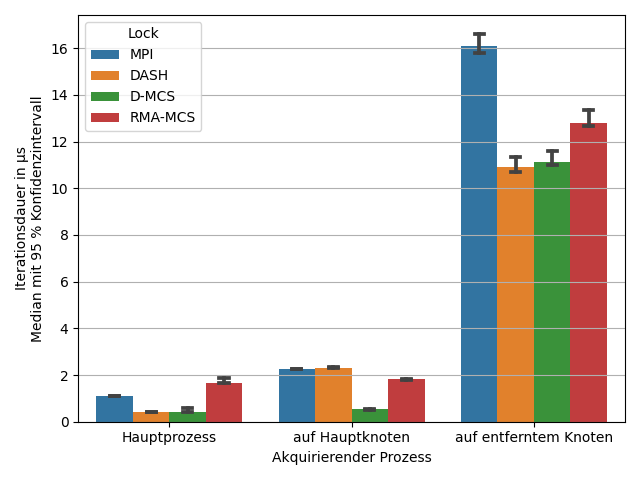
\includegraphics[width=\textwidth]{benchmarks/intelmpi/baseline/UPB-lock_count=1000-latency}
        \caption{Iterationsdauer in \textmu{s}}
        \label{ben:baseline_upb_latency}
    \end{subfigure}
    \begin{subfigure}{.5\textwidth}
        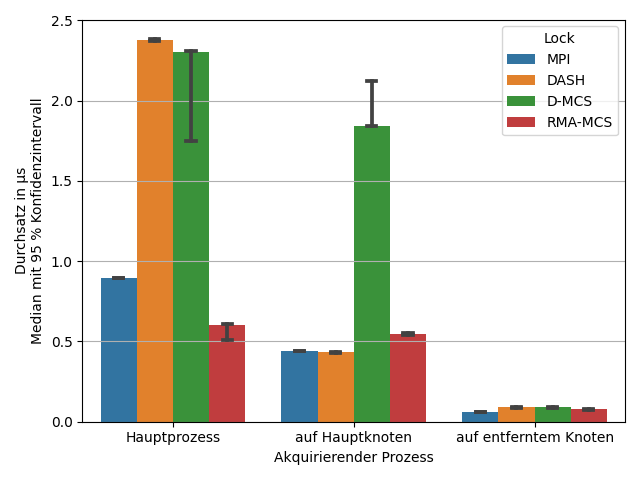
\includegraphics[width=\textwidth]{benchmarks/intelmpi/baseline/UPB-lock_count=1000-throughput}
        \caption{Durchsatz in Mio/s}
        \label{ben:baseline_upb_throughput}
    \end{subfigure}
    \caption{UPB der Basislocks}
    \label{ben:baseline_upb}
\end{benchmark}

\autoref{ben:baseline_upb_latency} zeigt,
wie lange es durchschnittlich dauert,
einen freien Lock zu akquirieren.
\autoref{ben:baseline_upb_throughput} hingegen zeigt umgerechnet,
wie viele Millionen freie Locks pro Sekunde akquiriert werden können.
Da es für diese Locks keinen Unterschied macht,
welcher Prozess der Vorgänger war,
sind in den beiden Abbildungen die Messungen unabhängig vom Vorgänger zusammengefasst.
Die Konfidenzintervalle beziehen sich hier somit auf 24 Messungen,
statt wie sonst auf 8.

In den Abbildungen sieht man deutlich den Einfluss von entfernten Speicherzugriffen auf die Performance.
Wenn der Hauptprozess des Locks auf einem anderen Knoten läuft
als der Prozess,
der den Lock akquiriert und freigibt,
sind alle Locks deutlich langsamer.
Beim Intel-MPI-Lock und \texttt{dash::Mutex} macht es darüber hinaus einen großen Unterschied,
ob der Prozess selbst der Hauptprozess
oder ein anderer Prozess auf dem Hauptknoten ist.
Der Grund hierfür ist leider nicht bekannt.
Zumindest bei \texttt{dash::Mutex} liegt es jedenfalls nicht an dem verwendeten Algorithmus,
denn sowohl \texttt{dash::Mutex}
als auch D-MCS müssen in diesem Benchmark nur zwei \gls{mpi}-Operationen ausführen:
ein \texttt{MPI\_Fetch\_and\_op} zum Akquirieren
und ein \texttt{MPI\_Compare\_and\_swap} zum Freigeben (jeweils mit \texttt{MPI\_Win\_flush}).
In \autoref{sec:optimierung_bestehender_locks} wird gezeigt,
dass eine Reimplementierung des Algorithmus aus \texttt{dash::Mutex} dieses Verhalten nicht aufweist.

Außerdem zeigt der \gls{upb},
dass ein freier RMA-MCS-Lock immer etwas langsamer ist
als ein freier D-MCS-Lock.
% Das ist auch zu erwarten.
Da RMA-MCS eine hierarchische Version des D-MCS mit zwei Hierarchieebenen ist,
muss bei einem freien Lock sowohl der lokale Lock
als auch der globale Lock akquiriert werden,
während D-MCS nur aus einem globalen Lock besteht.
\autoref{ben:baseline_upb_latency} zeigt allerdings,
dass der Overhead
von RMA-MCS gegenüber D-MCS
nur bei etwa 1,5~\textmu{s} liegt und zwar unabhängig davon,
auf welchem Knoten der Prozess läuft.

\clearpage

\subsection{Leerer kritischer Abschnitt (ECSB)}
\label{sec:ecsb}

Der Benchmark mit leerem kritischen Abschnitt (engl. \gls{ecsb}) ist
% in der Literatur
sehr verbreitet \cite{RH-Lock} \cite{HCLH-Lock} \cite{FC-MCS-Lock} \cite{HMCS-Lock},
vermutlich, weil er sehr einfach ist.
In einer Schleife akquiriert jeder Prozess den Lock
und gibt ihn direkt wieder frei.
Das ist zwar nicht sehr realistisch,
dafür beeinflusst aber nur der Lock selbst die Messung.
% denn es gibt keinen Overhead durch andere Operationen.

\begin{benchmark}[h]
    \begin{subfigure}{.5\textwidth}
        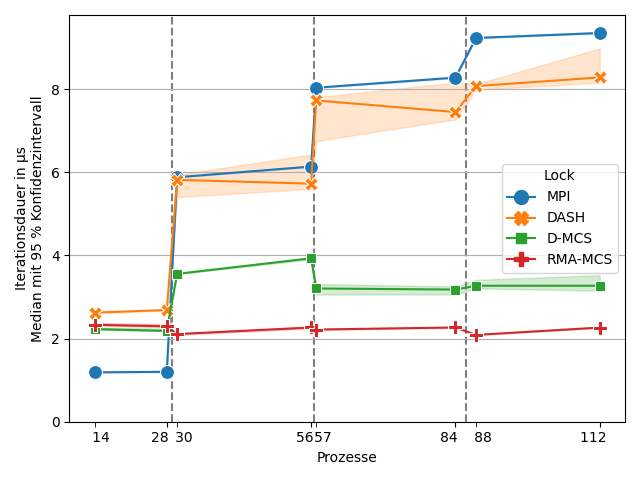
\includegraphics[width=\textwidth]{benchmarks/intelmpi/baseline/ECSB-latency}
        \caption{Iterationsdauer in \textmu{s}}
        \label{ben:baseline_ecsb_latency}
    \end{subfigure}
    \begin{subfigure}{.5\textwidth}
        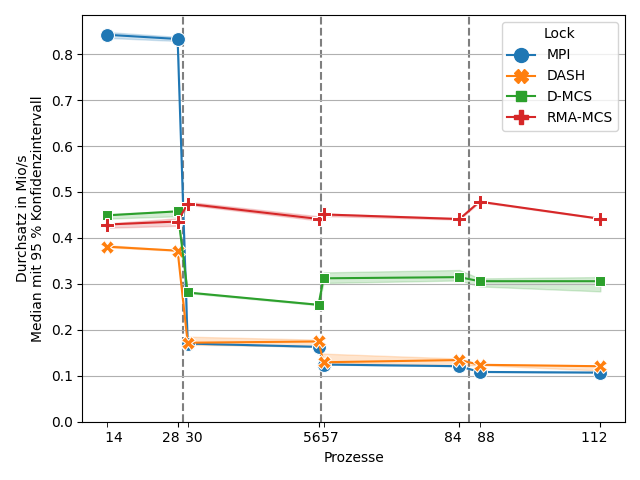
\includegraphics[width=\textwidth]{benchmarks/intelmpi/baseline/ECSB-throughput}
        \caption{Durchsatz in Mio/s}
        \label{ben:baseline_ecsb_throughput}
    \end{subfigure}
    \caption{ECSB der Basislocks (\ecsburl)}
    \label{ben:baseline_ecsb}
\end{benchmark}

\autoref{ben:baseline_ecsb} zeigt die Performance der Locks im \gls{ecsb}.
Man sieht,
dass in diesem Benchmark der Lock aus Intel-MPI bei Weitem am schnellsten ist,
solange nur ein Rechenknoten beteiligt ist.
Hier besteht offenbar großes Optimierungspotenzial bei den anderen Locks.
Jedes Mal,
wenn ein weiterer Rechenknoten hinzukommt
(bei 30, 57 und 88 Prozessen)
nimmt die Geschwindigkeit des MPI-Locks jedoch stark ab.
\texttt{dash::Mutex} zeigt ein sehr ähnliches Verhalten.
Hier ist allerdings auffällig,
dass dieser Lock hohe Schwankungen aufweist.
D-MCS und RMA-MCS sind bei mehreren Knoten deutlich schneller,
da sie direkte Speicherzugriffe
statt \gls{rma}-Operationen in den Warteschleifen verwenden (siehe \autoref{sec:mpi_fortschritt}).

Es wird auch deutlich,
dass Zugriffe auf entfernten Speicher vermieden werden sollten.
D-MCS unterscheidet nicht zwischen Prozessen auf demselben und anderen Knoten.
Die Performance nimmt daher bei 30 Prozessen deutlich ab,
da dann mehr als ein Rechenknoten beteiligt ist,
bleibt aber bei weiteren Knoten relativ konstant.
RMA-MCS verhält sich als einzige Implementierung stabil,
unabhängig von der Anzahl der Prozesse und Rechenknoten.

Da beim \gls{ecsb} außerhalb des kritischen Abschnitts nichts gemacht wird,
versuchen ständig Prozesse den kritischen Abschnitt zu betreten
und der Lock ist nie frei.
Die \gls{Konkurrenz} (nicht gezeigt) ist daher bei allen Locks unabhängig von der Anzahl an Prozessen bei 100~\%.

\begin{benchmark}[h]
    \centering
    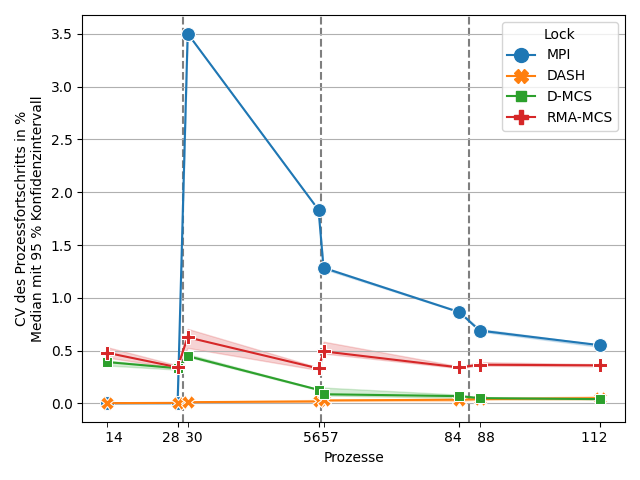
\includegraphics[width=.5\textwidth]{benchmarks/intelmpi/baseline/ECSB-fairness}
    \caption{Fairness der Basislocks im ECSB: CV des Fortschritts in \%}
    \label{ben:baseline_ecsb_fairness}
\end{benchmark}

\autoref{ben:baseline_ecsb_fairness} zeigt die Fairness der Locks im \gls{ecsb}.
Obwohl \texttt{dash::Mutex} und D-MCS beides Varianten des MCS-Locks sind
und theoretisch \gls{fifo} garantieren,
weist D-MCS eine etwas schlechtere Fairness auf,
die bei mehr und mehr Prozessen aber zu \texttt{dash::Mutex} aufholt.
RMA-MCS hat theoretisch eine beschränkte Unfairness von 50,
d.~h. es können maximal 50 andere Prozesse den ersten Prozess in der Warteschlange überholen.
Diese schlechtere theoretische Fairness könnte auch der Grund für die etwas schlechtere praktische Fairness sein.
Der Intel-MPI-Lock ist bei mehreren Knoten mit Abstand am unfairsten,
alle Locks sind mit einem Variationskoeffizienten von deutlich unter 5 \% allerdings ziemlich fair.

\subsection{Änderung des kritischen Arbeitsanteils (CCWB)}
\label{sec:ccwb}

Einen deutlich realistischeren Ansatz hat der \gls{ccwb}.
Auch dieser wird in verschiedenen Varianten häufig in der Literatur verwendet
\cite{RH-Lock} \cite{HCLH-Lock} \cite{FC-MCS-Lock} \cite{Cohort-Lock} \cite{RCL} \cite{HMCS-Lock} \cite{SANL}.
Die Idee bei diesem Benchmark ist es,
die \gls{Konkurrenz} zwischen den Prozessen zu erhöhen,
indem ein immer größerer Anteil der Arbeit im kritischen Abschnitt ausgeführt wird,
bis diese den Hauptteil der Rechenzeit beansprucht.
Zunächst ist der kritische Abschnitt leer.
Anders als beim \gls{ecsb} führen Prozesse aber vor dem Akquirieren des Locks einige Speicherzugriffe aus.
Diese Zugriffe repräsentieren den parallelisierbaren Anteil eines Programms
und werden im Folgenden als unkritische Arbeit $u$ bezeichnet.
Dann werden mehr und mehr Operationen im kritischen Abschnitt ausgeführt,
wodurch ein immer größerer Anteil des Programms serialisiert werden muss
und immer mehr Prozesse gleichzeitig den kritischen Abschnitt ausführen wollen.
Diese Operationen werden
% im Folgenden
als kritische Arbeit $k$ bezeichnet.
\autoref{fig:ccwb_code} zeigt den Quelltext einer \gls{ccwb}-Iteration.

\begin{figure}[h]
    \centering
    \begin{tabular}{c}\begin{lstlisting}
void ccwb(Lock &lock) {
  lock.acquire();
  for (int i = 0; i < k; i++)
    increment_non_atomically(sizeof(int) * i);
  lock.release();
  int u = distribution(generator);
  for (int i = 0; i < u; i++)
    increment_non_atomically(sizeof(int) * (k + i));
}

void increment_non_atomically(MPI_Aint disp) {
  // Der \enquote{rank} eines Prozesses, der wahrscheinlich auf einem anderen Knoten läuft.
  int remote_rank = (my_rank + p / 2) % p;
  int value;
  MPI_Get(&value, 1, MPI_INT, remote_rank, disp, 1, MPI_INT, win);
  MPI_Win_flush(remote_rank, win);
  value += 1;
  MPI_Put(&value, 1, MPI_INT, remote_rank, disp, 1, MPI_INT, win);
  MPI_Win_flush(remote_rank, win);
}
    \end{lstlisting}\end{tabular}
    \caption{Quelltext einer CCWB Iteration (\ccwburl)}
    \label{fig:ccwb_code}
\end{figure}

Ein spannender Punkt ist erreicht,
wenn kritische und unkritische Arbeit gleichermaßen an der Laufzeit beteiligt sind.
Das ist der Fall,
wenn die unkritische Arbeit $p - 1$ Mal so groß ist
wie die kritische Arbeit,
wobei $p$ die Anzahl der Prozesse ist.
Damit stellt die kritische Arbeit einen Anteil von $\frac{1}{p}$ der gesamten Arbeit eines Prozesses dar.
Dies ist der letzte Punkt,
an dem das Programm theoretisch perfekt parallelisierbar ist und wird im Folgenden als Equilibrium bezeichnet.

Man kann sich vorstellen,
dass im Optimalfall immer ein Prozess den kritischen Abschnitt ausführt,
während die anderen $p - 1$ Prozesse unkritische Arbeit ausführen.
In der Realität ist bereits etwas früher keine perfekte Parallelisierung mehr möglich,
da die Prozesse nicht immer zum perfekten Zeitpunkt den kritischen Abschnitt betreten möchten
und das Akquirieren und Freigeben des Locks zusätzlich Zeit benötigt.

Echte Anwendungen brauchen nicht zwischen jedem kritischen Abschnitt die gleiche Anzahl an Operationen.
Um das zu simulieren wird die tatsächliche Menge der unkritischen Arbeit zufällig bestimmt.
Ausgehend von einer minimalen Anzahl an Operationen $a$ bestimmt jeder Prozess in jeder Iteration
seine tatsächliche Arbeit $\tilde{a}$ indem er über eine Gleichverteilung eine Zufallszahl aus dem geschlossenen Intervall $[a; 2a]$ bestimmt.
Dies geschieht vor dem kritischen Abschnitt und nutzt \texttt{std::mt19937}%
\footnote{\url{https://en.cppreference.com/w/cpp/numeric/random/mersenne_twister_engine}}
und \texttt{std::uniform\_int\_distribution}%
\footnote{\url{https://en.cppreference.com/w/cpp/numeric/random/uniform_int_distribution}}
aus C++.
Die unkritische Arbeit $u$ bestimmt sich dann mit $u = \tilde{a} - k$.

Nun soll $a$ so gewählt werden,
dass das Equilibrium $e$ im Durchschnitt bei einer kritischen Arbeit von $k = 3$ erreicht ist.
So kann bei $k \in [0; 2]$ beobachtet werden,
wie der Lock sich verhält,
wenn die unkritische Arbeit dominiert
und bei $k \in [4; 5]$,
wie er sich verhält,
wenn die kritische Arbeit dominiert.
Da $\tilde{a}$ im Durchschnitt $1,5a$ ist,
berechnet sich $a$ mit: $a = p \cdot e / 1,5$,
in diesem Fall mit $e = 3$.
Für 112 Prozesse wird daher im Folgenden eine minimale Arbeit von $a = 224$ verwendet,
wodurch die tatsächliche Arbeit $\tilde{a}$ im Durchschnitt 336 ist.

Da die gesamte Arbeit $a$ gleich bleibt,
hätte eine theoretisch perfekte Lock-Implementier-ung
eine durchschnittliche Iterationsdauer von $max(\frac{1,5a}{p}, k)$,
multipliziert mit der Dauer einer Operation.
Solange das Equilibrium noch nicht erreicht ist,
ist das Programm perfekt parallelisierbar,
hat also eine Iterationsdauer von $\frac{1,5a}{p}$ ($\frac{\text{Durchschnittliche Arbeit}}{\text{Anzahl Prozesse}}$).
Sobald das Equilibrium erreicht ist,
gilt $\frac{k}{1,5a} = \frac{1}{p} \iff \frac{1,5a}{p} = k$.
Die kritische und unkritische Arbeit tragen dann gleichermaßen zur Laufzeit bei.
Nach dem Equilibrium hängt die Iterationsdauer linear von $k$ ab.

Als Operation wird sowohl im kritischen Abschnitt
als auch außerhalb mit \texttt{MPI\_Get} auf einen Speicherbereich eines Prozesses auf einem anderen Knoten zugegriffen,
der Wert inkrementiert
und mit \texttt{MPI\_Put} zurückgeschrieben.
In einem normalen Programm würde man hierfür \texttt{MPI\_Accumulate} verwenden,
um mit nur einem entfernten Zugriff den Wert atomar zu erhöhen,
aber da ein Lock normalerweise nicht-atomare Operationen schützt,
werden für diesen Benchmark zwei nicht-atomare Operationen verwendet.
So werden nacheinander die Werte an $\tilde{a}$ verschiedenen entfernten Speicheradressen inkrementiert.

Wichtig ist dabei,
dass nicht alle Prozesse auf dem Speicher desselben Prozesses arbeiten.
Ohne \gls{rdma} ist der Zielprozess an einer \gls{rma}-Operation beteiligt.
Wenn dann alle Prozesse ständig auf den Speicher desselben Prozesses zugreifen,
ist keine echte Parallelisierung möglich,
da dieser Prozess die Anfragen aller Prozesse beantworten muss.
Jeder Prozess hat daher einen anderen \enquote{Partner},
auf dessen Speicher er arbeitet.

\clearpage

\begin{benchmark}[h]
    \begin{subfigure}{.5\textwidth}
        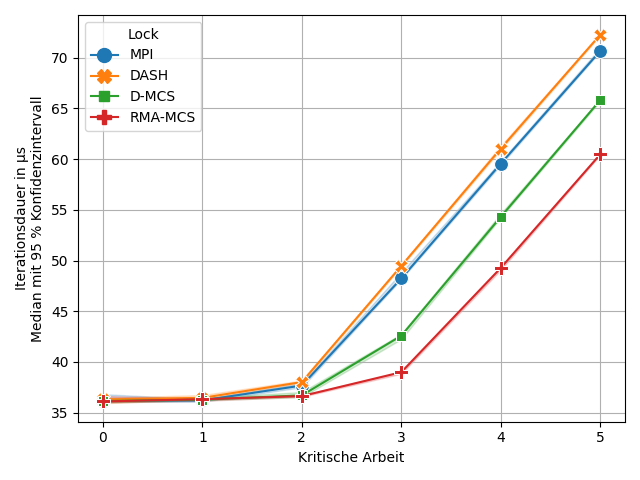
\includegraphics[width=\textwidth]{benchmarks/intelmpi/baseline/CCWB-processes=112-latency}
        \caption{Iterationsdauer in \textmu{s}}
        \label{ben:baseline_ccwb_112_latency}
    \end{subfigure}
    \begin{subfigure}{.5\textwidth}
        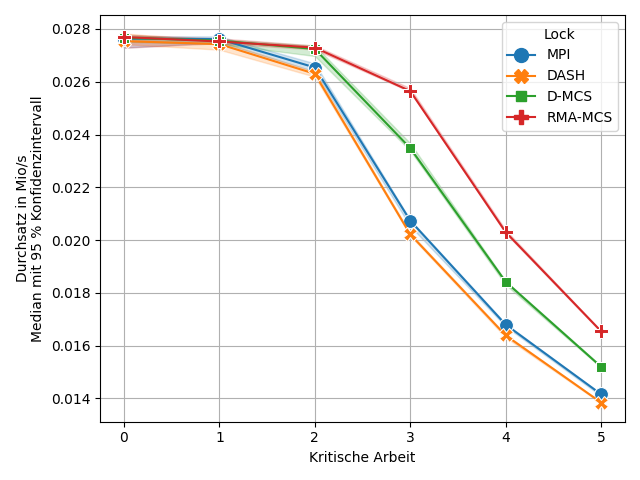
\includegraphics[width=\textwidth]{benchmarks/intelmpi/baseline/CCWB-processes=112-throughput}
        \caption{Durchsatz in Mio/s}
        \label{ben:baseline_ccwb_112_throughput}
    \end{subfigure}
    \begin{subfigure}{.5\textwidth}
        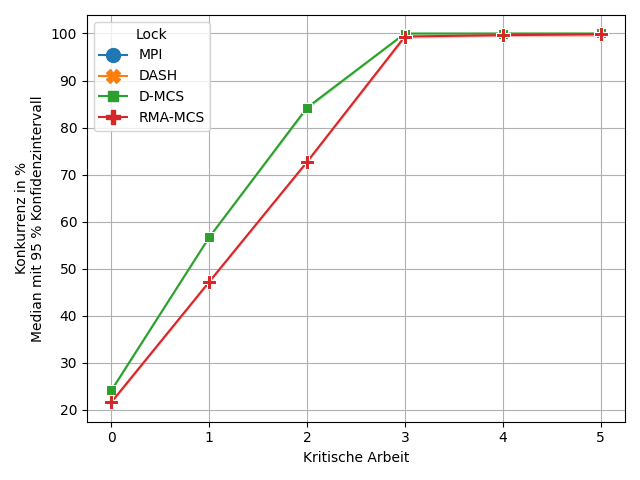
\includegraphics[width=\textwidth]{benchmarks/intelmpi/baseline/CCWB-processes=112-contention}
        \caption{Konkurrenz in \%}
        \label{ben:baseline_ccwb_112_contention}
    \end{subfigure}
    \begin{subfigure}{.5\textwidth}
        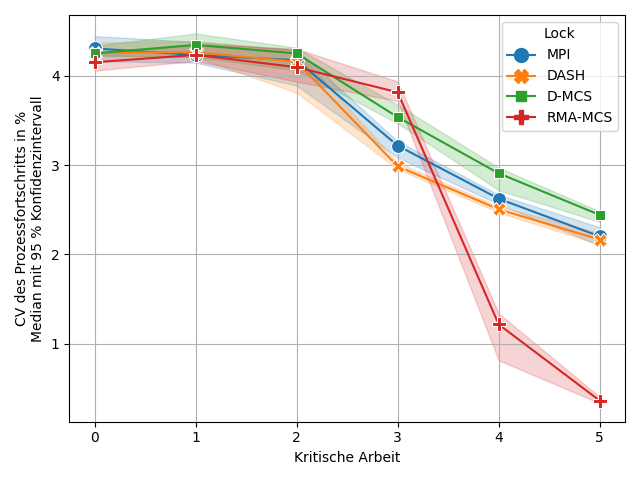
\includegraphics[width=\textwidth]{benchmarks/intelmpi/baseline/CCWB-processes=112-fairness}
        \caption{Fairness: CV des Fortschritts in \%}
        \label{ben:baseline_ccwb_112_fairness}
    \end{subfigure}
    \caption{CCWB der Basislocks mit 112 Prozessen}
    \label{ben:baseline_ccwb_112}
\end{benchmark}

\autoref{ben:baseline_ccwb_112_latency} und \autoref{ben:baseline_ccwb_112_throughput}
zeigen die Geschwindigkeit der Basislocks im \gls{ccwb} bei 112 Prozessen,
also vier voll ausgelasteten Knoten.
Ähnlich wie beim \gls{ecsb} liegen der \gls{mpi}-Lock und \texttt{dash::Mutex} nah beieinander,
während D-MCS und RMA-MCS deutlich schneller sind.
Allerdings ist in diesem Benchmark \texttt{dash::Mutex} etwas langsamer als der \gls{mpi}-Lock.
Es ist auch ersichtlich,
dass D-MCS und RMA-MCS einen deutlich geringeren Overhead haben
als die anderen beiden Locks,
da das Equilibrium bei ihnen noch nicht bei einer kritischen Arbeit von 2 einsetzt,
sondern erst später.
Dies geht auch aus \autoref{ben:baseline_ccwb_112_contention} hervor,
auch wenn die \gls{Konkurrenz} für die Locks aus den Bibliotheken \gls{mpi} und DASH nicht gemessen werden kann.

Die Fairness der Locks in \autoref{ben:baseline_ccwb_112_fairness} ist deutlich schlechter
und hat deutlich größere Konfidenzintervalle
als beim \gls{ecsb} in \autoref{ben:baseline_ecsb_fairness}.
Der Grund hierfür ist wahrscheinlich,
dass durch die geringere \gls{Konkurrenz} die Locks immer wieder frei werden.
Bei freien Locks macht es,
wie der \gls{upb} in \autoref{ben:baseline_upb} gezeigt hat,
einen großen Unterschied,
ob der akquirierende Prozess auf dem Hauptknoten läuft.
Solche Prozesse können freie Locks schneller akquirieren,
da keine entfernten Speicherzugriffe benötigt werden
und sind damit im Durchschnitt etwas schneller,
was zu einer höheren Unfairness führt.
Das erklärt auch,
warum die Fairness deutlich besser wird,
sobald das Equilibrium erreicht ist.

Darüber hinaus hat der \gls{ccwb} einen deutlich größeren Zufallsanteil,
da die Arbeit,
die jeder Prozess ausführen muss,
für jede Iteration aus einem recht großen Intervall bestimmt wird
und vollständig aus entfernten Speicherzugriffen besteht.
Auch der \gls{upb} hat bereits in \autoref{ben:baseline_upb_latency} gezeigt,
dass die Geschwindigkeit von entfernten Speicherzugriffen deutlich höheren Schwankungen unterliegt
als die von Lokalen.
Das könnte die ungenauen Konfidenzintervalle in \autoref{ben:baseline_ccwb_112_fairness} erklären.
Trotz der schlechteren Fairness haben alle Locks auch vor dem Equilibrium immer noch einen Variationskoeffizienten von unter 5~\%
und sind damit relativ fair.

\begin{benchmark}[h]
    \begin{subfigure}{.5\textwidth}
        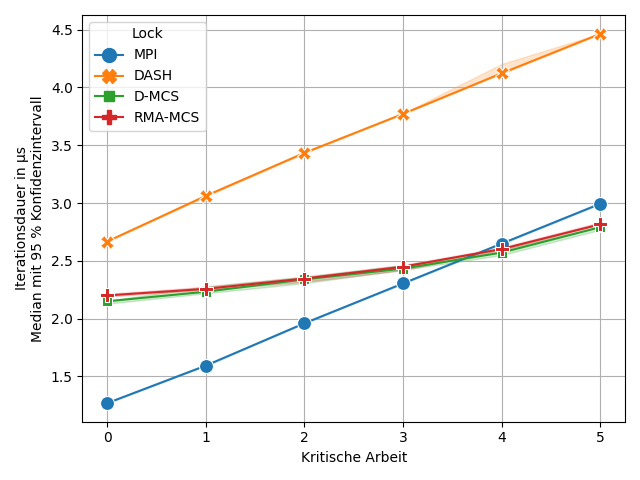
\includegraphics[width=\textwidth]{benchmarks/intelmpi/baseline/CCWB-processes=28-latency}
        \caption{Iterationsdauer in \textmu{s}}
        \label{ben:baseline_ccwb_28_latency}
    \end{subfigure}
    \begin{subfigure}{.5\textwidth}
        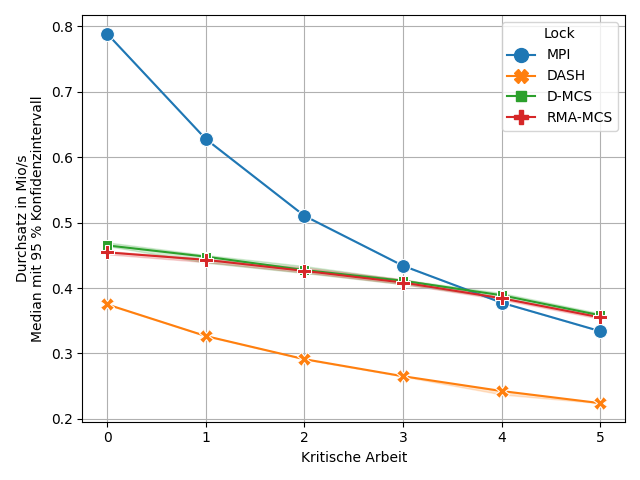
\includegraphics[width=\textwidth]{benchmarks/intelmpi/baseline/CCWB-processes=28-throughput}
        \caption{Durchsatz in Mio/s}
        \label{ben:baseline_ccwb_28_throughput}
    \end{subfigure}
    \begin{subfigure}{.5\textwidth}
        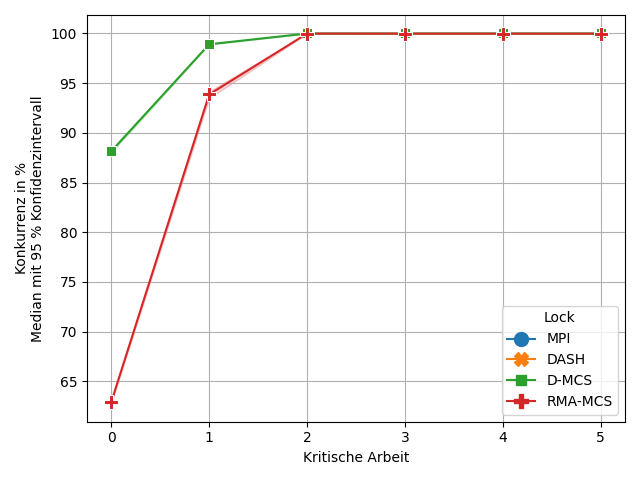
\includegraphics[width=\textwidth]{benchmarks/intelmpi/baseline/CCWB-processes=28-contention}
        \caption{Konkurrenz in \%}
        \label{ben:baseline_ccwb_28_contention}
    \end{subfigure}
    \begin{subfigure}{.5\textwidth}
        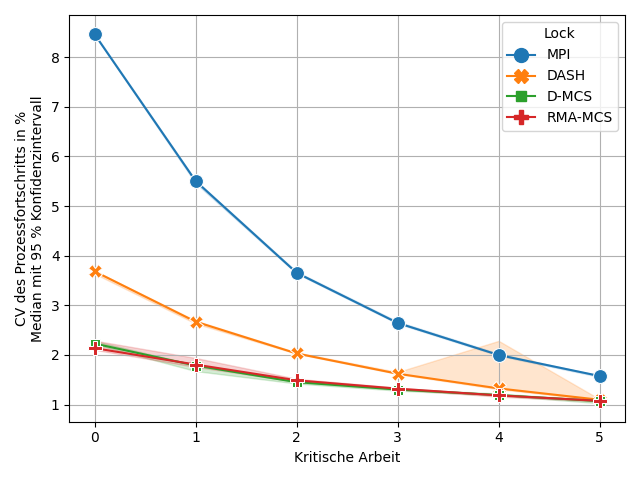
\includegraphics[width=\textwidth]{benchmarks/intelmpi/baseline/CCWB-processes=28-fairness}
        \caption{Fairness: CV des Fortschritts in \%}
        \label{ben:baseline_ccwb_28_fairness}
    \end{subfigure}
    \caption{CCWB der Basislocks mit 28 Prozessen}
    \label{ben:baseline_ccwb_28}
\end{benchmark}

Um das beim \gls{ecsb} identifizierte Optimierungspotenzial
bei der Nutzung von nur einem Knoten näher zu untersuchen,
zeigt \autoref{ben:baseline_ccwb_28} den \gls{ccwb} mit 28 Prozessen.
Da nur ein Knoten an dem Benchmark beteiligt ist,
handelt es sich bei den Operationen vor und in dem kritischen Abschnitt nun um lokale Operationen.
Da lokale Operationen deutlich schneller als entfernte Operationen sind,
sieht man den Overhead der Locks stärker.
Dabei macht es einen Unterschied,
welcher Anteil dieses Overheads auf dem kritischen Pfad (also quasi im kritischen Abschnitt)
und welcher außerhalb liegt.

Overhead außerhalb des kritischen Pfades hat denselben Effekt wie eine höhere unkritische Arbeit:
Die Iterationsdauer wird unabhängig von der Menge der kritischen Arbeit um eine Konstante erhöht.
Overhead auf dem kritischen Pfad führt zusätzlich dazu,
dass das Equilibrium früher erreicht ist,
wodurch die Iterationsdauer früher linear mit der kritischen Arbeit steigt.
Selbst wenn der Anteil der kritischen Arbeit klein ist,
ist Overhead auf dem kritischen Pfad schlechter,
weil es trotzdem passieren kann,
dass mehrere Prozesse zufällig gleichzeitig den kritischen Abschnitt betreten möchten,
wodurch sich der Overhead auf dem kritischen Pfad auf mehr als einen Prozess auswirken kann.
Umso höher der Anteil der kritischen Arbeit ist,
umso wahrscheinlicher ist es,
dass so ein Fall auftritt
und ab dem Equilibrium betrifft der Overhead auf dem kritischen Pfad immer alle Prozesse.
Umso mehr Prozesse beteiligt sind,
umso höher ist tendenziell der Anteil der kritischen Arbeit,
da sich die unkritische Arbeit auf mehr Prozesse verteilen kann (siehe auch \textit{Amdahl's Law} aus \cite{Amdahl's-law}).
Für eine gute Skalierbarkeit,
besonders im \gls{hpc}-Bereich mit Tausenden von Prozessen,
ist daher ein möglichst geringer Overhead vor allem auf dem kritischen Pfad wichtig.

\autoref{ben:baseline_ccwb_28_latency} zeigt deutlich,
dass der \gls{mpi}-Lock und \texttt{dash::Mutex} bei nur einem Knoten einen so hohen kritischen Overhead aufweisen,
dass dieser auch ohne kritische Arbeit die unkritische Arbeit von $avg(\tilde{a}) = 84$ \texttt{MPI\_Put}- und \texttt{MPI\_Get}-Operationen (jeweils mit \texttt{MPI\_Win\_flush}) dominiert.
D-MCS und RMA-MCS hingegen erreichen erst bei einer kritischen Arbeit von 1 bzw. 2 das Equilibrium,
wie \autoref{ben:baseline_ccwb_28_contention} zeigt.
Dafür weisen diese Locks einen deutlich höheren unkritischen Overhead als der \gls{mpi}-Lock auf,
sodass sie bei geringer kritischer Arbeit trotzdem langsamer sind.
Überraschenderweise ist das Equilibrium bei D-MCS und RMA-MCS nicht in \autoref{ben:baseline_ccwb_28_latency} zu sehen.
Zu erwarten wäre bei den beiden Locks ein plötzlicher starker linearer Anstieg der Iterationsdauer ab einer kritischen Arbeit von 1 bzw. 2,
mit derselben Steigung wie bei den anderen beiden Locks.
Der kritische Overhead der beiden Locks nimmt anscheinend ab,
wenn der kritische Abschnitt größer wird.
Dies wird bei der Optimierung des D-MCS in \autoref{sec:optimierung_bestehender_locks} näher untersucht.

Bei der Fairness schneidet der \gls{mpi}-Lock
mit einem Variationskoeffizienten von über 8~\%
deutlich schlechter ab
als die anderen Locks,
welche weiterhin unter 5~\% bleiben,
wie \autoref{ben:baseline_ccwb_28_fairness} zeigt.

\subsection{Vor dem Akquirieren warten (WBAB)}
\label{sec:wbab}

Der \gls{ecsb} hat gezeigt,
dass die Basislocks auf verteiltem Speicher so viel kritischen Overhead haben,
dass selbst bei leerem kritischen Abschnitt 100~\% \gls{Konkurrenz} herrscht.
Daher lässt sich die \gls{Konkurrenz} auch variieren,
indem mehr und mehr Arbeit außerhalb eines leeren kritischen Abschnitts ausgeführt wird.
Das hat gegenüber dem \gls{ccwb} den Vorteil,
dass weniger Operationen ausgeführt werden,
die zur Ungenauigkeit der Messergebnisse beitragen
und dass der Overhead des Locks einen größeren Teil der Laufzeit ausmacht,
wodurch er besser zu sehen ist.
Der Nachteil ist,
dass dieser Benchmark nicht so realistisch ist
wie der \gls{ccwb},
da ein leerer kritischer Abschnitt in der Praxis keinen Sinn macht.

Beim \gls{wbab} warten Prozesse
vor dem Akquirieren des Locks
für eine zufällig bestimmte Zeit
in einer Schleife
(\wbaburl).
Diese Zeit wird
wie beim \gls{ccwb}
aus dem geschlossenen Intervall $[w; 2w]$ bestimmt.
Dabei ist $w$
(die minimale Wartezeit in Nanosekunden)
ein Parameter des Benchmarks.
Die tatsächliche Wartezeit $\tilde{w}$ ist damit im Durchschnitt $1,5w$.
Der kritische Abschnitt ist wie beim \gls{ecsb} leer.
Anders als beim \gls{ccwb} werden in der Wartezeit vor dem kritischen Abschnitt
keine \gls{mpi}-Operationen ausgeführt.
Das ermöglicht zum einen eine beliebige Präzision,
da die Wartezeit auch in Schritten erhöht werden kann,
die kleiner sind
als eine \gls{mpi}-Operation dauert
und zum anderen eine genaue Bestimmung des Overheads bei Messung der Iterationsdauer,
da die Wartezeit in einer Zeiteinheit angegeben ist,
statt in einer Anzahl von Operationen.

Der \gls{wbab} in dieser Form kommt nicht in der Literatur über \gls{numa}-Locks vor.
Der Grund dafür ist wahrscheinlich,
dass auf gemeinsamem Speicher der Overhead der Locks geringer ist,
wodurch die \gls{Konkurrenz} bei einem leeren kritischen Abschnitt schon bei geringer Wartezeit stark abnimmt.
Bei einer Änderung der Wartezeit im Bereich von wenigen Nanosekunden
würde dann bereits die Ermittlung der Systemzeit das Messergebnis zu sehr verfälschen.
Außerdem spielt bei gemeinsamem Speicher häufig der \gls{Zwischenspeicher}-\gls{Kohaerenz}-Mechanismus eine große Rolle
und es ist wichtig zu messen,
ob der Speicher,
auf den im kritischen Abschnitt zugegriffen wird,
bereits im \gls{Zwischenspeicher} liegt.
Das ist besonders bei delegierenden Locks ein wichtiger Faktor
(siehe \autoref{sec:delegation_locks}).
In \cite{FC-MCS-Lock}, \cite{Cohort-Lock} und \cite{HMCS-Lock}
werden ähnliche Benchmarks mit einer festen Anzahl an Operationen
im kritischen Abschnitt verwendet.
Nur \cite{RMA-RW} behandelt verteilten Speicher
und nutzt einen sehr ähnlichen Benchmark mit leerem kritischen Abschnitt
und Wartezeit nach dem Freigeben des Locks.
All diese Benchmarks variieren aber die Anzahl der Prozesse und nicht die Wartezeit.
Sie nutzen eine willkürlich gewählte Wartezeit,
die unabhängig von der Anzahl der Prozesse ist.

Da bei verteiltem Speicher deutlich mehr Prozessoren zur Verfügung stehen
als bei gemeinsamem Speicher,
sollte der Benchmark auch mit beliebig vielen Prozessen ausgeführt werden können.
Daher wird beim \gls{wbab},
wie beim \gls{ccwb},
die Wartezeit abhängig von der Anzahl von Prozessen bestimmt.
Zunächst wird eine minimale Wartezeit von $w = 0$ verwendet,
um bei maximaler \gls{Konkurrenz} zu beginnen.
Dieses Szenario ist identisch zum \gls{ecsb}.
Anschließend wird $w$ so gewählt,
dass der Durchschnitt der tatsächlichen Wartezeit $\tilde{w}$,
ausgehend von $0,25~\text{\textmu{s}} \cdot p$ in jedem Schritt verdoppelt wird.
$p$ ist hierbei wieder die Anzahl der Prozesse.
Durch das exponentielle Wachstum von $\tilde{w}$ kann fast das gesamte Spektrum der \gls{Konkurrenz} untersucht werden.
Die \gls{Konkurrenz} nimmt nämlich bei zunehmender Wartezeit immer langsamer ab,
was durch das schnelle Wachstum ausgeglichen wird.

Wenn die Prozesse in der Wartezeit einfach nur in einer Schleife die Zeit prüfen,
garantiert \gls{mpi} in dieser Zeit keinen Fortschritt für andere Prozesse,
die auf den Speicher dieses Prozesses zugreifen wollen,
da ohne \gls{rdma} das Betriebssystem des Zielrechners an der Kommunikation beteiligt sein muss (vgl. \autoref{sec:mpi_fortschritt}).
Das ist vor allem ein Problem,
wenn der wartende Prozess der Hauptprozess eines Locks ist,
da die meisten Locks bei jeder Akquisition des Locks auf den Speicher dieses Prozesses zugreifen.

\begin{benchmark}[h]
    \begin{subfigure}{.5\textwidth}
        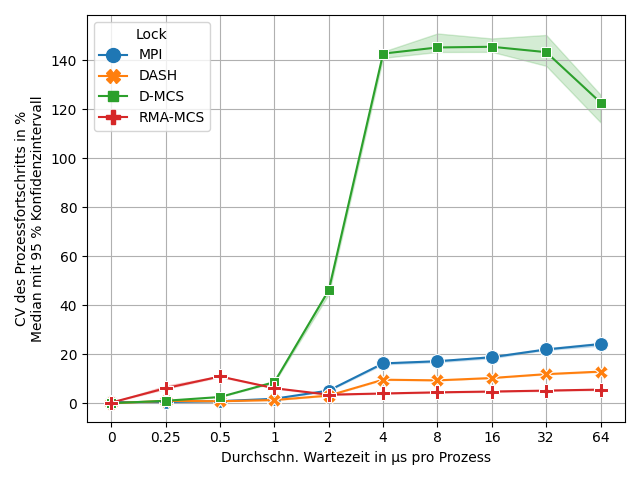
\includegraphics[width=\textwidth]{benchmarks/intelmpi/baseline/WBAB-processes=112,mpi_progress=0-fairness}
        \caption{112 Prozesse}
        \label{ben:baseline_wbab_112_no_progress_fairness}
    \end{subfigure}
    \begin{subfigure}{.5\textwidth}
        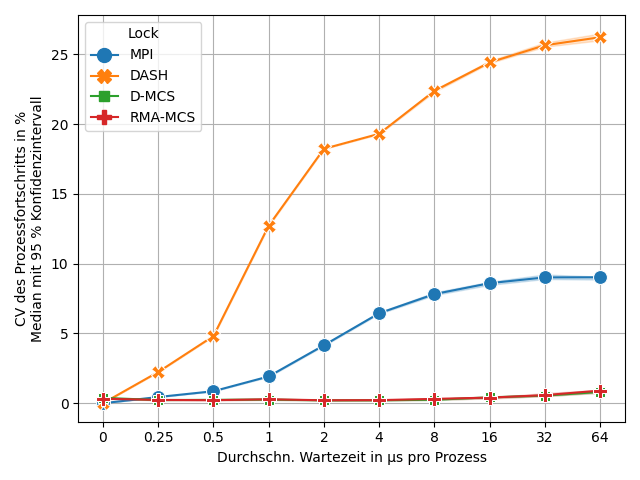
\includegraphics[width=\textwidth]{benchmarks/intelmpi/baseline/WBAB-processes=28,mpi_progress=0-fairness}
        \caption{28 Prozesse}
        \label{ben:baseline_wbab_28_no_progress_fairness}
    \end{subfigure}
    \caption{Fairness im WBAB ohne \texttt{MPI\_Iprobe}: CV des Fortschritts in \%}
    \label{ben:baseline_wbab_no_progress_fairness}
\end{benchmark}

Wie \autoref{ben:baseline_wbab_112_no_progress_fairness} zeigt,
führt das zu extremer Unfairness.
Dabei sind die Locks verschieden schwer betroffen:
D-MCS erreicht bei 112 Prozessen einen Variationskoeffizienten von mehr als 140~\%.
Das bedeutet die Standardabweichung ist über 40~\% höher als der Durchschnitt an ausgeführten Iterationen.
Die minimale Anzahl und der Median an ausgeführten Iterationen
bei einer durchschnittlichen Wartezeit von 4~\textmu{s}
waren bei D-MCS im Durchschnitt der acht Wiederholungen gerade einmal 99.25 und 102.75,
während der schnellste Prozess im Durchschnitt 1966 Iterationen schaffte.
% mean(min) 99.25
% mean(max) 1966.0
% mean(median) 102.75
Das liegt daran,
dass sich in der Wartezeit nur der Hauptprozess
(evtl. auch die anderen Prozesse auf dem Hauptknoten)
in die Warteschlange einreihen konnte.
Der Hauptprozess muss nicht nur nicht warten,
um sich in die Warteschlange einzureihen,
sondern hat im Durchschnitt auch weniger Vorgänger in der Warteschlange,
da sich in seiner Wartezeit kein anderer Prozess einreihen konnte.

\texttt{dash::Mutex} ist hiervon weniger stark betroffen,
obwohl dieser auch eine Variante des MCS-Locks ist.
Hier wird beim Freigeben des Locks immer eine \gls{cas}-Operation ausgeführt.
Auch diese kann nicht ausgeführt werden,
während der Hauptprozess wartet,
sodass in dieser Zeit gar kein Prozess kritischen Fortschritt machen kann.
Das bedeutet aber auch,
dass sich die Warteschlange in dieser Zeit nicht abbaut,
wodurch auch der Hauptprozess im Durchschnitt mehr Vorgänger hat.
Dadurch,
dass der Hauptprozess sich länger in der Warteschlange befindet,
gibt es auch ein größeres Zeitintervall,
in dem Prozesse sich in die Warteschlange einreihen können.
\texttt{dash::Mutex} wird also nicht so unfair wie D-MCS,
leidet aber auch unter massiven Einbußen bei der Geschwindigkeit.

RMA-MCS kommt von allen Locks am besten mit der Situation klar.
Da dieser Lock \gls{numa} berücksichtigt,
ist nicht bei jeder Akquisition des Locks ein Zugriff auf den Hauptprozess notwendig.
% Durch die stark reduzierte Kommunikation mit dem Hauptprozess
Dadurch hat RMA-MCS weniger Einbußen,
sowohl bei Geschwindigkeit als auch Fairness.
Nur bei einer durchschnittlichen Wartezeit von 0,5~\textmu{s} steigt der Variationskoeffizient bei RMA-MCS knapp über 10~\%.

Bei 28 Prozessen,
also auf nur einem Rechenknoten ist das Bild deutlich anders
(vgl. \autoref{ben:baseline_wbab_28_no_progress_fairness}).
Das es keine Zugriffe auf entfernten Speicher gibt,
gibt es auch keine Probleme mit Fortschrittsgarantien.
Trotzdem haben \texttt{dash::Mutex} und der Intel-MPI-Lock eine schlechte Fairness.
Der Grund hierfür ist unbekannt,
allerdings verschwindet dieser Effekt bei einer Reimplementierung des Algorithmus aus \texttt{dash::Mutex} in \autoref{sec:optimierung_bestehender_locks}.
Das erinnert an die höhere Latenz beim Akquirieren eines freien Locks
durch einen nicht-Hauptprozess auf dem Hauptknoten im \gls{upb}.
Auch dort gab es bei \texttt{dash::Mutex} und dem MPI-Lock einen Unterschied zwischen dem Hauptprozess
und anderen Prozessen auf demselben Knoten,
nicht aber bei D-MCS und RMA-MCS.
Und auch dieses Verhalten verschwindet bei einer Reimplementierung von \texttt{dash::Mutex}.

Das Szenario ist insgesamt durch den leeren kritischen Abschnitt
und der vollständigen Abwesenheit von entfernten Speicherzugriffen außerhalb des kritischen Abschnitts nicht sehr realistisch.
Trotzdem ist es in echten Anwendungen durchaus möglich,
dass Prozesse außerhalb von kritischen Abschnitten vor allem lokale Berechnungen durchführen,
die ohne \gls{mpi}-Operationen auskommen.
In solchen Fällen wäre,
genau wie in diesem Benchmark,
kein Programmfortschritt möglich.
Daher sollten bei der Verwendung von \gls{rma} in \gls{mpi}-Anwendungen lange Abschnitte ohne \gls{mpi}-Operationen vermieden werden.
Wie in \autoref{sec:mpi_fortschritt} gezeigt,
garantiert nicht jede \gls{mpi}-Operation Fortschritt.
Die Garantie hängt von der \gls{mpi}-Implementierung ab:
Weder in Intel-MPI,
noch in Open-MPI löst \texttt{MPI\_Win\_sync} das Problem,
in Open-MPI noch nicht einmal \texttt{MPI\_Win\_flush}.
Locks,
die \gls{numa} berücksichtigen,
sind hierdurch gegenüber anderen Lock-Algorithmen gleich doppelt im Vorteil.
Sie vermeiden neben langsamen entfernten Speicherzugriffen bei hinreichender \gls{Konkurrenz}
auch solche Fortschrittsprobleme.

Um die Probleme mit dem Programmfortschritt in \gls{wbab} zu lösen,
führen alle Prozesse in der Warteschleife \texttt{MPI\_Iprobe} mit \texttt{MPI\_ANY\_SOURCE} und \texttt{MPI\_ANY\_TAG} aus.
Es würde zwar reichen,
wenn nur der Hauptprozess das tun würde,
aber im Benchmark sollen alle Prozesse fair behandelt werden.
Die Ergebnisse dieser beiden Varianten unterscheiden sich tatsächlich kaum.

\begin{benchmark}[h]
    \begin{subfigure}{.5\textwidth}
        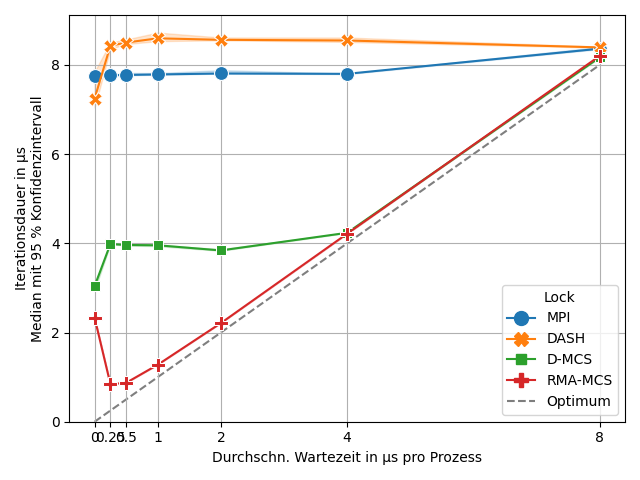
\includegraphics[width=\textwidth]{benchmarks/intelmpi/baseline/WBAB-processes=112,mpi_progress=1-latency}
        \caption{Iterationsdauer in \textmu{s}}
        \label{ben:baseline_wbab_112_latency}
    \end{subfigure}
    \begin{subfigure}{.5\textwidth}
        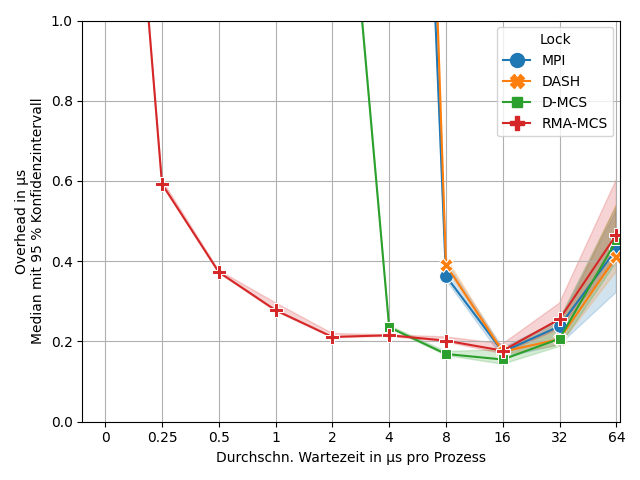
\includegraphics[width=\textwidth]{benchmarks/intelmpi/baseline/WBAB-processes=112,mpi_progress=1-overhead}
        \caption{Overhead in \textmu{s}}
        \label{ben:baseline_wbab_112_overhead}
    \end{subfigure}
    \begin{subfigure}{.5\textwidth}
        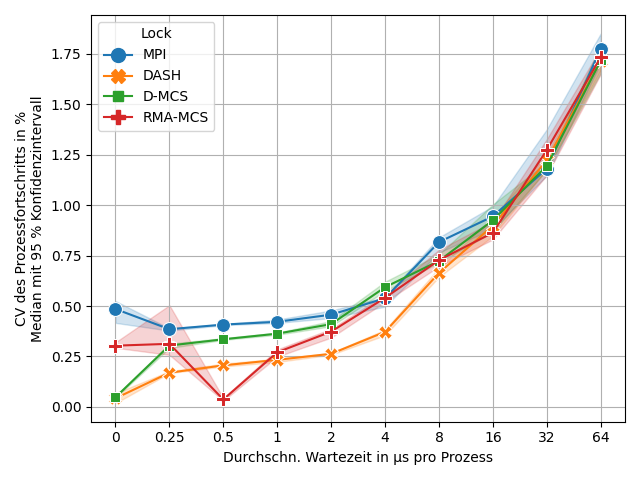
\includegraphics[width=\textwidth]{benchmarks/intelmpi/baseline/WBAB-processes=112,mpi_progress=1-fairness}
        \caption{Fairness: CV des Fortschritts in \%}
        \label{ben:baseline_wbab_112_fairness}
    \end{subfigure}
    \begin{subfigure}{.5\textwidth}
        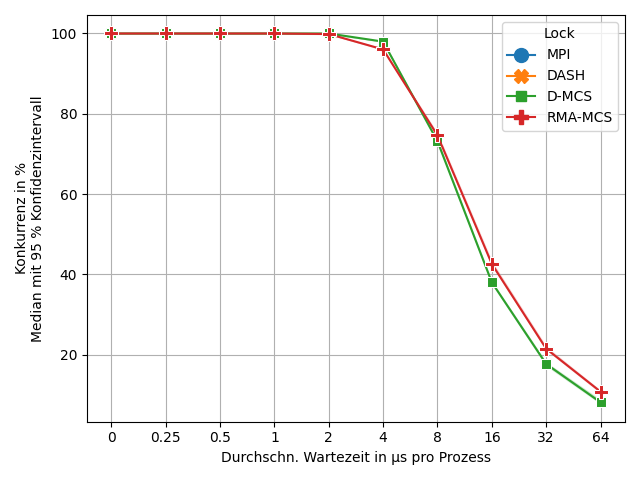
\includegraphics[width=\textwidth]{benchmarks/intelmpi/baseline/WBAB-processes=112,mpi_progress=1-contention}
        \caption{Konkurrenz in \%}
        \label{ben:baseline_wbab_112_contention}
    \end{subfigure}
    \caption{WBAB der Basislocks mit 112 Prozessen}
    \label{ben:baseline_wbab_112}
\end{benchmark}

\autoref{ben:baseline_wbab_112} zeigt die Performance der Locks im korrigierten \gls{wbab}.
Dabei sieht man in \autoref{ben:baseline_wbab_112_fairness},
dass die Fairnessprobleme durch \texttt{MPI\_Iprobe} behoben wurden:
Alle Prozesse sind fair,
mit Variationskoeffizienten von deutlich unter 2~\%.
Mit steigender Wartezeit steigt auch die Unfairness,
da Prozesse auf dem Hauptknoten etwas schneller sind.
Wenn die \gls{Konkurrenz} sinkt,
gibt es seltener eine Warteschlange,
die Fairnessgarantien durchsetzt.

Da in \autoref{ben:baseline_wbab_112_latency} sowohl die x-, als auch die y-Achse Mikrosekunden zeigen,
kann der kritische Overhead im \gls{wbab} quantifiziert werden.
Er entspricht der Iterationsdauer vor Eintreten des Equilibriums.
Das liegt daran,
dass vor Eintreten des Equilibriums die kritische Arbeit dominiert
und diese besteht im \gls{wbab} nur aus dem kritischen Overhead des Locks,
% da hier die kritische Arbeit dominiert.
% Die kritische Arbeit besteht im \gls{wbab} nur aus dem kritischen Overhead des Locks,
da der kritische Abschnitt leer ist.
% besteht die kritische Arbeit nur aus dem kritischen Overhead des Locks.
Da der kritische Overhead unabhängig von der Wartezeit ist,
bleibt auch die Iterationsdauer vor dem Einsetzen des Equilibriums relativ konstant.
Nur bei einer durchschnittlichen Wartezeit von 0~\textmu{s} gibt es größere Schwankungen.

Genau wie der \gls{ccwb},
zeigt der \gls{wbab},
dass der kritische Overhead vom \gls{mpi}-Lock und \texttt{dash::Mutex} deutlich höher ist
als der von D-MCS und RMA-MCS.
Erstere haben einen kritischen Overhead von knapp unter,
bzw. etwas über 8~\textmu{s}.
Der kritische Overhead von D-MCS und RMA-MCS ist deutlich niedriger:
bei etwa 4~\textmu{s} bzw. knapp unter 1~\textmu{s}.

\begin{benchmark}[!b]
    \begin{subfigure}{.5\textwidth}
        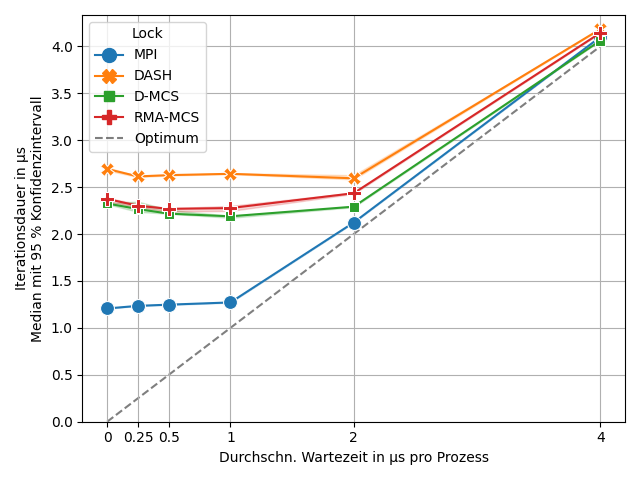
\includegraphics[width=\textwidth]{benchmarks/intelmpi/baseline/WBAB-processes=28,mpi_progress=1-latency}
        \caption{Iterationsdauer in \textmu{s}}
        \label{ben:baseline_wbab_28_latency}
    \end{subfigure}
    \begin{subfigure}{.5\textwidth}
        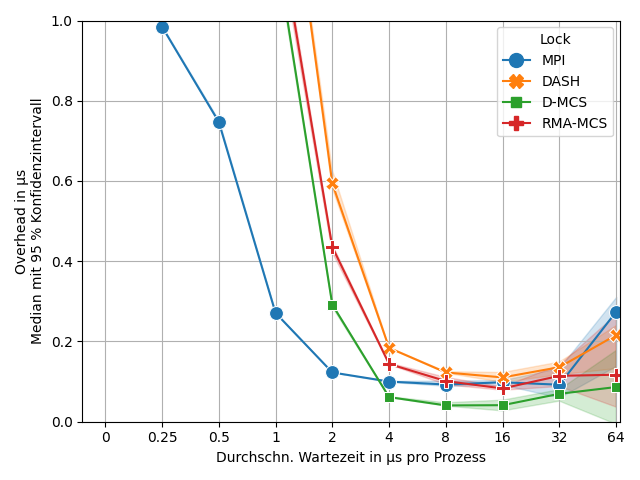
\includegraphics[width=\textwidth]{benchmarks/intelmpi/baseline/WBAB-processes=28,mpi_progress=1-overhead}
        \caption{Overhead in \textmu{s}}
        \label{ben:baseline_wbab_28_overhead}
    \end{subfigure}
    \begin{subfigure}{.5\textwidth}
        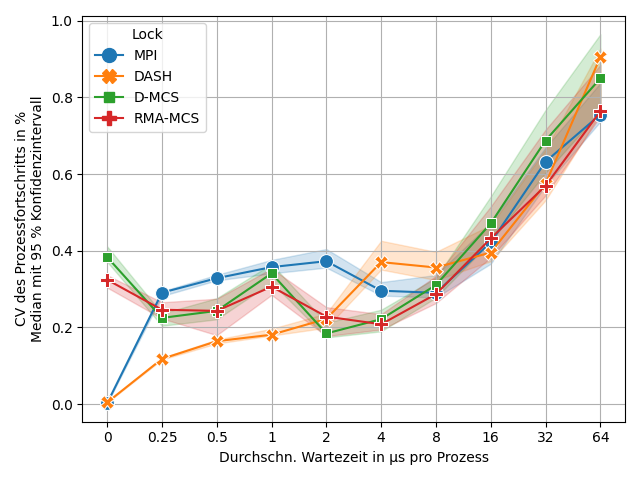
\includegraphics[width=\textwidth]{benchmarks/intelmpi/baseline/WBAB-processes=28,mpi_progress=1-fairness}
        \caption{Fairness: CV des Fortschritts in \%}
        \label{ben:baseline_wbab_28_fairness}
    \end{subfigure}
    \begin{subfigure}{.5\textwidth}
        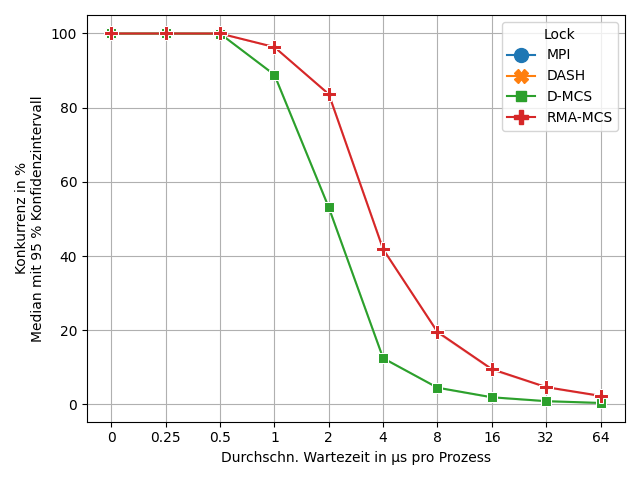
\includegraphics[width=\textwidth]{benchmarks/intelmpi/baseline/WBAB-processes=28,mpi_progress=1-contention}
        \caption{Konkurrenz in \%}
        \label{ben:baseline_wbab_28_contention}
    \end{subfigure}
    \caption{WBAB der Basislocks mit 28 Prozessen}
    \label{ben:baseline_wbab_28}
\end{benchmark}

Zusätzlich enthält \autoref{ben:baseline_wbab_112_latency} das theoretische Optimum,
welches der durchschnittlichen Wartezeit entspricht.
Da bei \gls{wbab} das theoretische Optimum bekannt ist,
kann der reine Overhead der Locks gezeigt werden,
indem das Optimum von der Iterationsdauer abgezogen wird.
Dieser Overhead wird in \autoref{ben:baseline_wbab_112_overhead} gezeigt.
Im Gegensatz zu \autoref{ben:baseline_wbab_112_latency},
geht hier die durchschnittliche Wartezeit bis 64~\textmu{s} pro Prozess,
wodurch die \gls{Konkurrenz} auf etwa 10~\% fällt
(vgl. \autoref{ben:baseline_wbab_112_contention}).
Eine noch höhere Wartezeit würde zwar die \gls{Konkurrenz} noch weiter senken,
aber eine Wartezeit von $64~\text{\textmu{s}} \cdot 112 \approx 7~\text{ms}$ ist bereits so groß,
dass das Messergebnis ungenau wird,
wie die Konfidenzintervalle zeigen.
Bei einer Laufzeit von einer Sekunde,
wobei 10~\% auch noch zum Aufwärmen verwendet werden,
schafft jeder Prozess bei dieser Wartezeit nur noch etwa 125 Iterationen.
Hinzu kommt,
dass bei sehr geringer \gls{Konkurrenz} immer mehr Zugriffe auf entfernten Speicher zum Overhead beitragen.
Das liegt daran,
dass immer mehr freie Locks akquiriert werden müssen
und die meisten Prozesse auf einem anderen Knoten laufen
als der Hauptprozess.
Entfernte Zugriffe haben größere Schwankungen,
was die Ungenauigkeit weiter erhöht.
Da sie auch langsam sind,
nimmt der Overhead ab einer \gls{Konkurrenz} von 40~\% wieder zu.

Die Betrachtung des Overheads auch bei höheren Wartezeiten zeigt,
dass auch nach Erreichen des Equilibriums der Overhead zunächst weiter abnimmt
und später wieder steigt.
Dabei sieht man in \autoref{ben:baseline_wbab_112_overhead},
dass bei geringer \gls{Konkurrenz} der D-MCS-Lock etwas besser ist
als der RMA-MCS-Lock.
Genau wie beim \gls{upb} sieht man hier den Nachteil der zwei Hierarchieebenen des RMA-MCS-Locks,
durch die ein Prozess bei geringer \gls{Konkurrenz} oft beide MCS-Locks nacheinander akquirieren muss,
was natürlich langsamer ist
als nur einen MCS-Lock zu akquirieren,
so wie es bei D-MCS der Fall ist.
Da einer der Locks aber nur lokal ist,
ist dieser Nachteil sehr klein.

Der Vollständigkeit halber zeigt \autoref{ben:baseline_wbab_28} den \gls{wbab} mit 28 Prozessen.
Wie auch in \gls{ecsb} und \gls{ccwb} ist der MPI-Lock bei nur einem Rechenknoten deutlich am schnellsten.
D-MCS und RMA-MCS sind nah beieinander auf Platz zwei und drei
und \texttt{dash::Mutex} am langsamsten.
Die Fairness ist wie bei 112 Prozessen mit einem Variationskoeffizienten von deutlich unter 1~\% sehr gut.

\section{Optimierung bestehender Locks}
\label{sec:optimierung_bestehender_locks}

Bevor \gls{numa}-Algorithmen auf verteilten Speicher portiert werden,
werden die in \autoref{ch:dist_locks} identifizierten Optimierungen auf die bestehenden Locks angewandt.
So können diese bei der Portierung direkt berücksichtigt werden.

Die bestehenden Locks enthalten zwei Varianten,
einen Lock weiterzugeben:
D-MCS und RMA-MCS nutzen hierfür \gls{rma},
während \texttt{dash::Mutex} hierfür Punkt-zu-Punkt-Kommunika-tion nutzt.
Um beide Varianten fair evaluieren zu können,
werden D-MCS in \autoref{sec:optimierung_dmcs} und \texttt{dash::Mutex} in \autoref{sec:optimierung_dash} optimiert.

In diesem Abschnitt wird der \gls{wbab} mit linear statt exponentiell steigender Wartezeit ausgeführt,
da für die Vergleiche vor allem die Iterationsdauer interessant ist
und so eine höhere Auflösung bei geringen Werten vorliegt.

\subsection{Optimierung von D-MCS}
\label{sec:optimierung_dmcs}

Der D-MCS-Lock ist bereits ein sehr optimierter Lock.
Dennoch wurden in dieser Arbeit einige Verbesserungen identifiziert,
die bereits in \autoref{fig:mcs_mpi_code} gezeigt wurden.

Erstens nutzt D-MCS nach Aufrufen von \texttt{MPI\_Accumulate} kein \texttt{MPI\_Win\_flush}
und auch keine sonstige Synchronisierungsfunktion.
Das betrifft zum einen das Benachrichtigen des Vorgängers beim Einreihen in die Warteschlange
und zum anderen die letzte Operation beim Weitergeben des Locks an einen Nachfolger.
Ohne Synchronisierungsfunktion ist aber nicht garantiert,
dass diese Operation überhaupt ausgeführt wird:

\clearpage

\foreignblockcquote{english}[Kapitel 11.7.3, S. 462]{MPI-3.1}{%
    \textins{A}n RMA communication may become enabled as soon as the corresponding
    put, get or accumulate call has executed, or as late as when the ensuing synchronization
    call is issued.}
Außerdem verletzt das \texttt{MPI\_Accumulate},
welches den Lock an den Nachfolger übergibt,
die \gls{mpi}-Spezifikation:
\foreignblockcquote{english}[Kapitel 11.3, S. 417]{MPI-3.1}{%
    \textins{RMA} operations are nonblocking: the
    call initiates the transfer, but the transfer may continue after the call returns. The transfer
    is completed, at the origin or both the origin and the target, when a subsequent synchronization
    call is issued by the caller on the involved window object \textelp{}.
    The local communication buffer of an RMA call should not be updated \textelp{} after the RMA call until the
    operation completes at the origin.}
Da es die letzte Operation in der \texttt{release}-Funktion ist,
wird nach dieser Operation der Speicher auf dem Stack freigegeben,
der an \texttt{MPI\_Accumulate} übergeben wurde.
Je nachdem,
wann die \gls{mpi}-Implementierung auf diesen Speicher zugreift,
ist der Speicher also invalide.

\begin{benchmark}[h]
    \begin{subfigure}{.5\textwidth}
        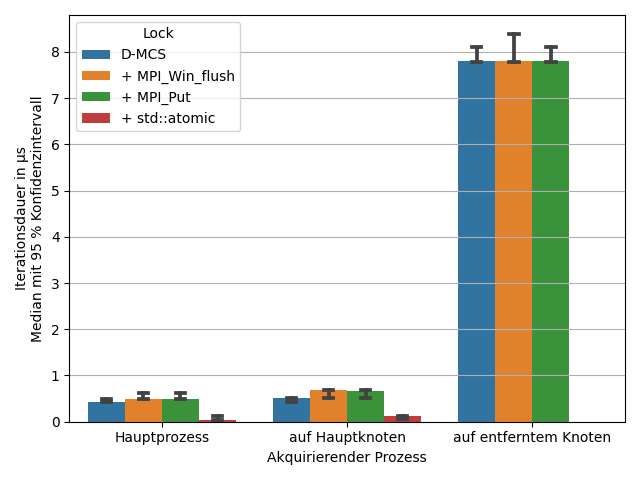
\includegraphics[width=\textwidth]{benchmarks/intelmpi/dmcs-optimization/UPB-lock_count=1000-latency}
        \caption{UPB}
        \label{ben:dmcs_upb_latency}
    \end{subfigure}
    \begin{subfigure}{.5\textwidth}
        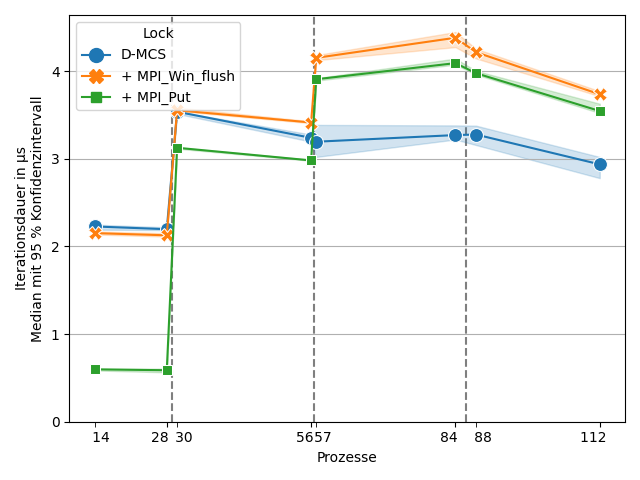
\includegraphics[width=\textwidth]{benchmarks/intelmpi/dmcs-optimization/ECSB-latency}
        \caption{ECSB}
        \label{ben:dmcs_ecsb_latency}
    \end{subfigure}
    \begin{subfigure}{.5\textwidth}
        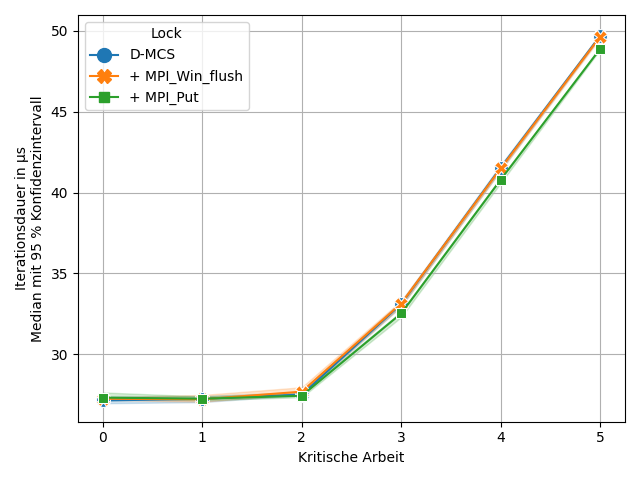
\includegraphics[width=\textwidth]{benchmarks/intelmpi/dmcs-optimization/CCWB-processes=112-latency}
        \caption{CCWB mit 112 Prozessen}
        \label{ben:dmcs_ccwb_112_latency}
    \end{subfigure}
    \begin{subfigure}{.5\textwidth}
        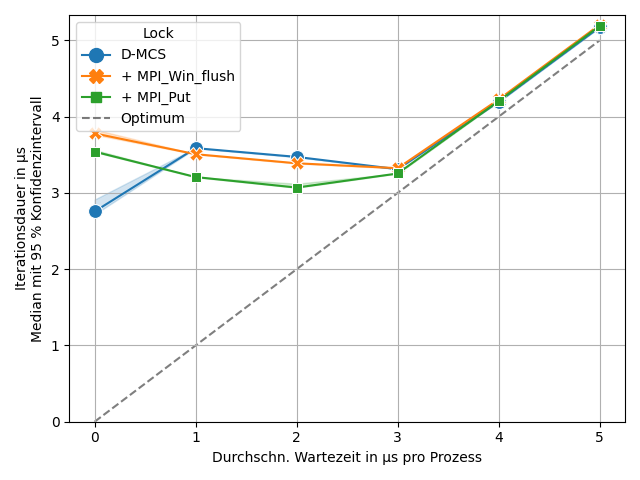
\includegraphics[width=\textwidth]{benchmarks/intelmpi/dmcs-optimization/WBAB-processes=112,mpi_progress=1-latency}
        \caption{WBAB mit 112 Prozessen}
        \label{ben:dmcs_wbab_112_latency}
    \end{subfigure}
    \caption{Iterationsdauer der D-MCS-Optimierungen in \textmu{s}}
    \label{fig:dmcs_latency}
\end{benchmark}

Als Korrektur und erste Optimierung werden daher beide \texttt{MPI\_Accumulate}-Operationen direkt im Anschluss mit \texttt{MPI\_Win\_flush} vollständig ausgeführt.
Zwar würde eine lokale Ausführung mit \texttt{MPI\_Win\_flush\_local} reichen,
aber da sich die Operationen jeweils auf dem kritischen Pfad befinden,
ist eine direkte vollständige Ausführung wünschenswert.

\autoref{fig:dmcs_latency} zeigt,
dass diese Änderung einen interessanten Effekt hat:
Wenn keine Arbeit ausgeführt wird,
wie es im \gls{ecsb} (vgl. \autoref{ben:dmcs_ecsb_latency})
und \gls{wbab} (vgl. \autoref{ben:dmcs_wbab_112_latency}) ohne Wartezeit der Fall ist,
wird der Lock langsamer.
Ansonsten wird er schneller.
Dies ist in \autoref{ben:dmcs_ccwb_112_latency} allerdings kaum zu erkennen,
da die Verbesserung nur klein ist.

Die Verbesserung ist von der unkritischen Arbeit abhängig,
da ohne unkritische Arbeit der Lock direkt wieder akquiriert wird,
wobei auch \texttt{MPI\_Win\_flush} zum Einsatz kommt.
In diesem Fall verursacht die Änderung also nur unnötigen Overhead.
Wenn aber zunächst unkritische Arbeit ausgeführt wird,
kann sich dadurch die Ausführung von \texttt{MPI\_Accumulate} verzögern
und damit der kritische Pfad verlängern.

Die zweite Optimierung ist die nicht-atomare Übergabe von Locks aus \autoref{sec:non_atomic_lock_passing}.
Statt der beiden \texttt{MPI\_Accumulate}-Operationen wird \texttt{MPI\_Put} verwendet.
Dadurch muss die \gls{mpi}-Implementierung nicht mehr prüfen,
ob mehrere parallele \gls{rma}-Operationen auf diesen Speicherbereich zugreifen.
Parallele Zugriffe sind an diesen Stellen sowieso durch den Algorithmus ausgeschlossen.
% Das kann auch tatsächlich in beiden Fällen nicht der Fall sein.
Die Optimierung realisiert auch das in \autoref{sec:ecsb} identifizierte Optimierungspotenzial auf einem einzelnen Rechenknoten.
Sowohl in \autoref{ben:dmcs_ecsb_latency}
als auch in \autoref{ben:dmcs_ccwb_28} wird das deutlich.
Der so optimierte D-MCS schlägt sogar den Intel-MPI-Lock,
welcher auf einem Rechenknoten zuvor die beste Performance hatte
(siehe \autoref{ben:baseline_opt_ccwb_28_latency}).

\begin{benchmark}[h]
    \begin{subfigure}{.5\textwidth}
        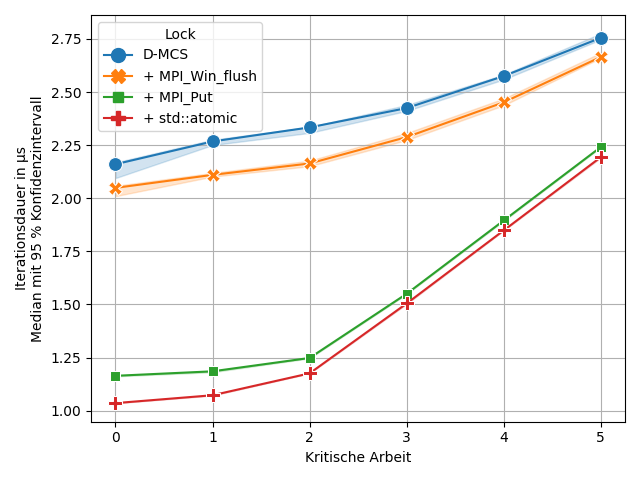
\includegraphics[width=\textwidth]{benchmarks/intelmpi/dmcs-optimization/CCWB-processes=28-latency}
        \caption{Iterationsdauer in \textmu{s}}
        \label{ben:dmcs_ccwb_28_latency}
    \end{subfigure}
    \begin{subfigure}{.5\textwidth}
        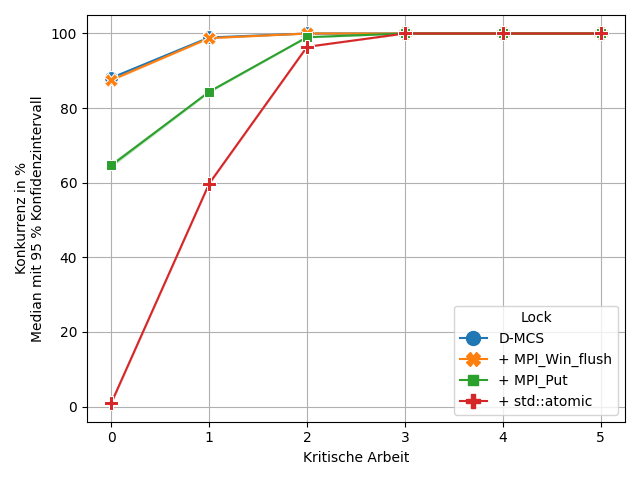
\includegraphics[width=\textwidth]{benchmarks/intelmpi/dmcs-optimization/CCWB-processes=28-contention}
        \caption{Konkurrenz in \%}
        \label{ben:dmcs_ccwb_28_contention}
    \end{subfigure}
    \caption{CCWB der D-MCS-Optimierungen mit 28 Prozessen}
    \label{ben:dmcs_ccwb_28}
\end{benchmark}

Die letzte Optimierung ist das Ersetzen der \gls{mpi}-Operationen durch C++ \texttt{std::atomic}.
Damit ist zwar nur lokale,
also auf den Knoten beschränkte Kommunikation möglich,
aber wie in \autoref{sec:mpi_shared_mem} erwähnt,
kann so ein Lock als Baustein für \gls{numa}-Locks wie den Cohort-Lock \cite{Cohort-Lock} dienen.
Außerdem wird hierdurch noch einmal verdeutlicht,
welchen Overhead die lokale Nutzung von \gls{rma}-Operationen mit sich bringt.
Das ist besonders in \autoref{ben:dmcs_upb_latency} ersichtlich.

\clearpage

\subsection{Optimierung von dash::Mutex}
\label{sec:optimierung_dash}

Damit der Algorithmus von \texttt{dash::Mutex} leichter optimiert werden kann,
wird er zunächst wie die anderen Locks mit einem eigenen \gls{mpi}-\gls{Fenster} reimplementiert.
Der Quelltext der Reimplementierung ist in \autoref{fig:dash_code} zu sehen.
Dabei ändern sich einige Implementierungsdetails
und da der Lock nun nicht mehr in die Bibliothek DASH eingebunden ist,
entfallen einige lokale Operationen,
wie etwa das Laden von Metadaten des DASH-Teams.

\begin{figure}[h]
    \begin{subfigure}{.5\textwidth}
        \centering
        \begin{tabular}{c}\begin{lstlisting}
win_mem->next = -1;
MPI_Win_sync(win);

// Finde Vorgänger
int pred;
MPI_Fetch_and_op(
  &my_rank, &pred, MPI_INT,
  main_rank, tail_disp,
  MPI_REPLACE, win);
MPI_Win_flush(main_rank, win);

if (pred != -1) {
  // Reihe nach Vorgänger ein
  int result;
  MPI_Fetch_and_op(
    &my_rank, &result, MPI_INT,
    pred, next_disp,
    MPI_REPLACE, win);
  MPI_Win_flush(pred, win);

  // Warte auf Vorgänger
  MPI_Recv(NULL, 0, MPI_UINT8_T,
           predecessor, 0, comm,
           MPI_STATUS_IGNORE);
}
        \end{lstlisting}\end{tabular}
        \caption{Akquirieren des Locks (\texttt{acquire})}
        \label{fig:dash_acquire}
    \end{subfigure}
    \begin{subfigure}{.5\textwidth}
        \centering
        \begin{tabular}{c}\begin{lstlisting}
constexpr int NULL_RANK = -1;
int old_value;
MPI_Compare_and_swap(
  &NULL_RANK, &my_rank, &old_value,
  MPI_INT, main_rank, tail_disp, win);
MPI_Win_flush(main_rank, win);

// Die Warteschlange ist leer
if (old_value == my_rank) return;
// Warte auf Nachfolger
int succ;
do {
  int flag; // Garantiere Fortschritt
  MPI_Iprobe(
    MPI_ANY_SOURCE, MPI_ANY_TAG,
    comm, &flag, MPI_STATUS_IGNORE);

  MPI_Fetch_and_op(
    NULL, &successor, MPI_INT,
    my_rank, next_disp, MPI_NO_OP, win);
  MPI_Win_flush(my_rank, win);
} while(succ == -1);
// Benachrichtige Nachfolger
MPI_Send(NULL, 0, MPI_UINT8_T,
         successor, 0, comm);
        \end{lstlisting}\end{tabular}
        \caption{Freigeben des Locks (\texttt{release})}
        \label{fig:dash_release}
    \end{subfigure}
    \caption{Implementierung von \texttt{dash::Mutex}}
    \label{fig:dash_code}
\end{figure}

Durch das Entfallen dieser Operationen nimmt vor allem der unkritische Overhead ab.
Das sieht man besonders im \gls{ccwb} und \gls{wbab} auf einem Rechenknoten
(in \autoref{ben:dash_ccwb_28_latency} und \autoref{ben:dash_wbab_28_latency}):
Beide Implementierungen erreichen bei einer kritischen Arbeit von 0,
bzw. einer Wartezeit von 2~\textmu{s} das Equilibrium,
haben also vergleichbaren kritischen Overhead,
die Reimplementierung ist aber immer etwas schneller.
Durch diese Reimplementierung verschwindet auch das in \autoref{sec:upb} festgestellte Verhalten,
dass das Akquirieren eines freien Locks länger dauert,
wenn es sich nicht um den Hauptprozess handelt (siehe \autoref{ben:dash_upb_latency}).

\begin{benchmark}[!h]
    \begin{subfigure}{.5\textwidth}
        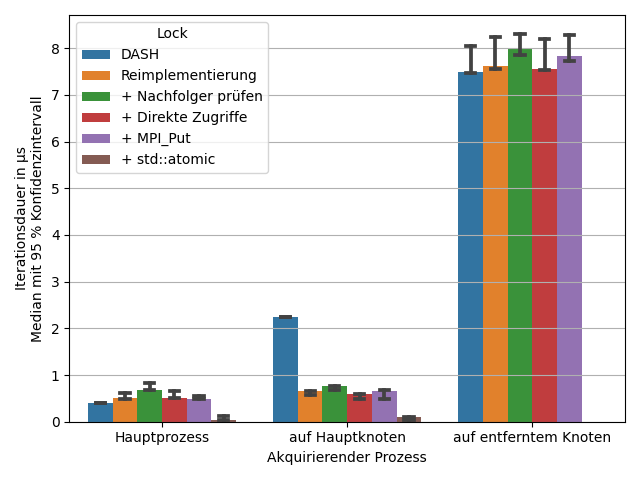
\includegraphics[width=\textwidth]{benchmarks/intelmpi/dash-optimization/UPB-lock_count=1000-latency}
        \caption{UPB}
        \label{ben:dash_upb_latency}
    \end{subfigure}
    \begin{subfigure}{.5\textwidth}
        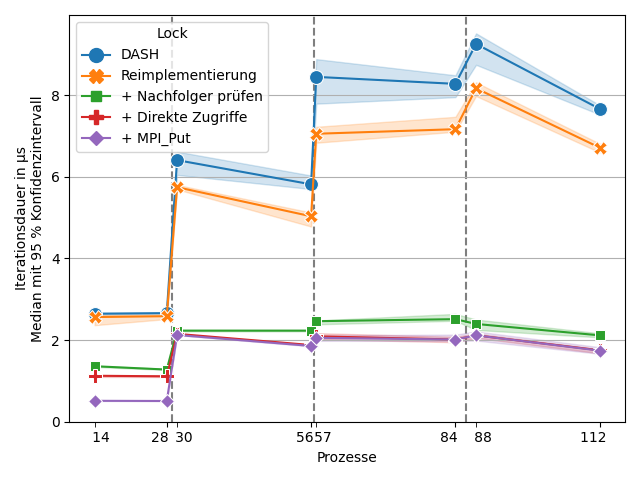
\includegraphics[width=\textwidth]{benchmarks/intelmpi/dash-optimization/ECSB-latency}
        \caption{ECSB}
        \label{ben:dash_ecsb_latency}
    \end{subfigure}
    \begin{subfigure}{.5\textwidth}
        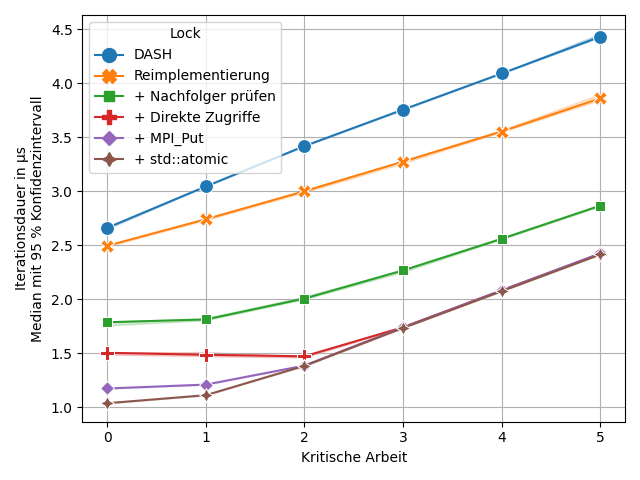
\includegraphics[width=\textwidth]{benchmarks/intelmpi/dash-optimization/CCWB-processes=28-latency}
        \caption{CCWB mit 28 Prozessen}
        \label{ben:dash_ccwb_28_latency}
    \end{subfigure}
    \begin{subfigure}{.5\textwidth}
        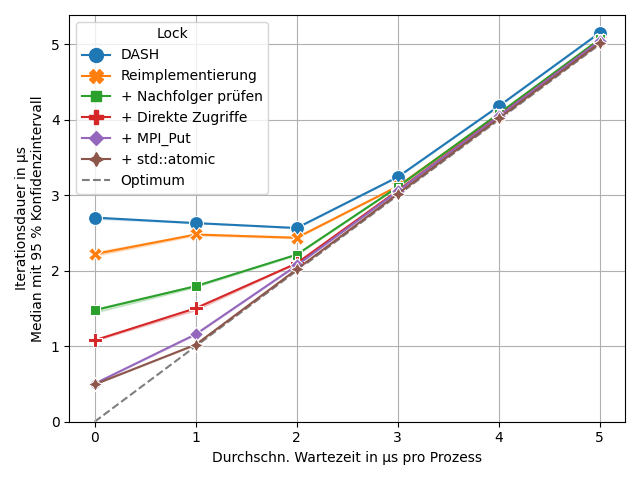
\includegraphics[width=\textwidth]{benchmarks/intelmpi/dash-optimization/WBAB-processes=28,mpi_progress=1-latency}
        \caption{WBAB mit 28 Prozessen}
        \label{ben:dash_wbab_28_latency}
    \end{subfigure}
    \begin{subfigure}{.5\textwidth}
        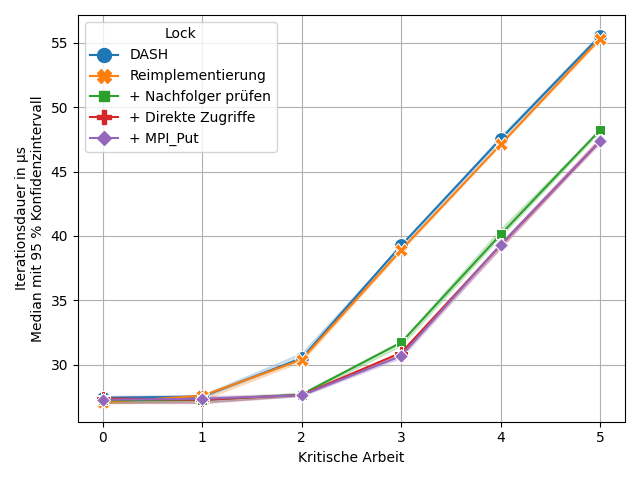
\includegraphics[width=\textwidth]{benchmarks/intelmpi/dash-optimization/CCWB-processes=112-latency}
        \caption{CCWB mit 112 Prozessen}
        \label{ben:dash_ccwb_112_latency}
    \end{subfigure}
    \begin{subfigure}{.5\textwidth}
        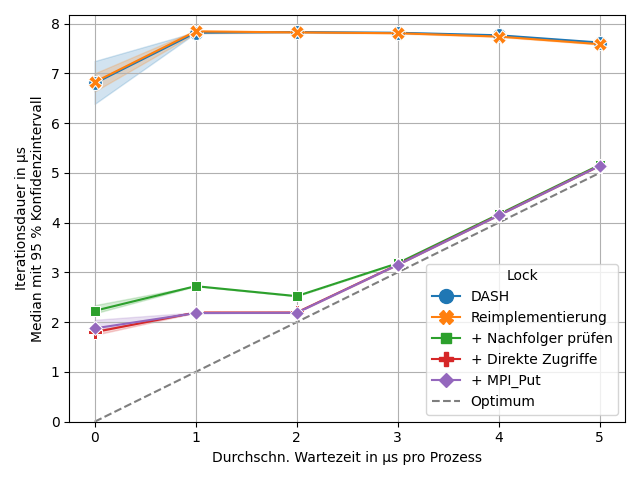
\includegraphics[width=\textwidth]{benchmarks/intelmpi/dash-optimization/WBAB-processes=112,mpi_progress=1-latency}
        \caption{WBAB mit 112 Prozessen}
        \label{ben:dash_wbab_112_latency}
    \end{subfigure}
    \caption{Iterationsdauer der DASH-Optimierungen in \textmu{s}}
    \label{fig:dash_latency}
\end{benchmark}

Das Hauptproblem an dem Algorithmus hinter \texttt{dash::Mutex} ist,
dass in \texttt{release} nicht,
wie bei einem MCS-Lock üblich,
mit einer lokalen Operation geprüft wird,
ob sich bereits ein Nachfolger registriert hat.
Stattdessen wird direkt versucht,
mit einer \gls{cas}-Operation auf den entfernten Speicher des Hauptprozesses
den Lock freizugeben.
Erst wenn diese Operation fehlschlägt,
wird mit \texttt{MPI\_Fetch\_and\_op} und \texttt{MPI\_NO\_OP} auf einen lokalen Nachfolger gewartet (\autoref{fig:dash_release}, Zeile 10-22).
Die erste Optimierung besteht daher darin,
in \texttt{release} bereits vor dem \gls{cas} mit \texttt{MPI\_Fetch\_and\_op} und \texttt{MPI\_NO\_OP} atomar zu prüfen,
ob lokal ein Nachfolger registriert ist.
Hier wird eine atomare \gls{mpi}-Funktion benötigt,
um einen \textit{memory consistency error} zu vermeiden,
wenn der Nachfolger genau im selben Moment Zeile 13-19 in \autoref{fig:dash_acquire} ausführt,
um sich zu registrieren.

Der \gls{upb} zeigt in \autoref{ben:dash_upb_latency},
dass diese Änderung bei einem freien Lock etwas langsamer ist,
da eine zusätzliche Operation ausgeführt wird,
die unnötig ist,
wenn es keinen Nachfolger gibt.
Da es sich aber nur um eine Lese-Operation handelt,
ist dieser zusätzliche Overhead sehr gering,
besonders wenn man ihn mit dem Overhead der Einbettung in DASH vergleicht.
Dafür verbessert diese Änderung die Performance in allen anderen Benchmarks drastisch:
Wenn es einen Nachfolger gibt,
wird eine \gls{cas}-Operation vermieden,
die deutlich langsamer ist als die atomare Lese-Operation,
die in diesem Fall sowieso im Anschluss ausgeführt würde.
Wenn mehrere Knoten beteiligt sind,
ist dieser Effekt sogar noch stärker,
da die \gls{cas}-Operation auf den Speicher des Hauptprozesses
und damit potenziell auf entfernten Speicher zugreift.

Als zweite Optimierung werden,
wie im D-MCS-Lock,
für Zugriffe auf lokalen Speicher direkte Speicherzugriffe verwendet (vgl. \autoref{fig:mcs_mpi_release}, Zeile 13-20).
Das betrifft nur das in der ersten Optimierung hinzugefügte \texttt{MPI\_Fetch\_and\_op}
und das Warten auf den Nachfolger (\autoref{fig:dash_release}, Zeile 18-21),
da \texttt{dash::Mutex} Punkt-zu-Punkt-Kommunikation für die Lockübergabe nutzt.
Diese Optimierung gleicht die kleine Verschlechterung im \gls{upb} wieder aus,
da ein direkter lesender Zugriff auf lokalen Speicher sehr schnell ist,
und auch in allen anderen Benchmarks verbessert sich dadurch die Geschwindigkeit.

Als drittes wird wie in \autoref{sec:optimierung_dmcs} \texttt{MPI\_Put} verwendet,
um sich beim Vorgänger zu registrieren (\autoref{fig:dash_acquire}, Zeile 15-18).
Anders als bei D-MCS ersetzt \texttt{MPI\_Put} hier ein \texttt{MPI\_Fetch\_and\_op} und nicht ein \texttt{MPI\_Accumulate}.
Warum \texttt{dash::Mutex} an dieser Stelle \texttt{MPI\_Fetch\_and\_op} verwendet ist nicht klar.
Diese Funktion liefert im Gegensatz zu \texttt{MPI\_Accumulate} den Wert zurück,
der vor der Operation an der Speicheradresse stand.
Dieser alte Wert (die lokale Variable \texttt{result}) wird aber gar nicht verwendet.
Diese Optimierung bringt anders als bei D-MCS nur eine relativ kleine Verbesserung bei mehreren Rechenknoten,
da die Übergabe des Locks an den Nachfolger Punkt-zu-Punkt-Kommunikation nutzt
und somit nicht betroffen ist.
Nach dem Registrieren beim Vorgänger müssen Prozesse typischerweise sowieso auf ihren Vorgänger warten.
Daher bringt es nichts,
wenn das Registrieren schneller ist.
Trotzdem verbessert sich die Performance bei nur einem Rechenknoten deutlich.
Zu prüfen,
ob mehrere parallele \gls{rma}-Operationen auf denselben Speicherbereich zugreifen,
verursacht demnach erheblichen Overhead bei der \gls{mpi}-Implementierung.

Als letzte Optimierung werden wieder alle \gls{mpi}-Operationen durch C++ \texttt{std::atomic} ersetzt,
wodurch dieser Lock wieder nur als Baustein für \gls{numa}-Locks wie den Cohort-Lock \cite{Cohort-Lock} dienen kann.

\begin{benchmark}[h]
    \begin{subfigure}{.5\textwidth}
        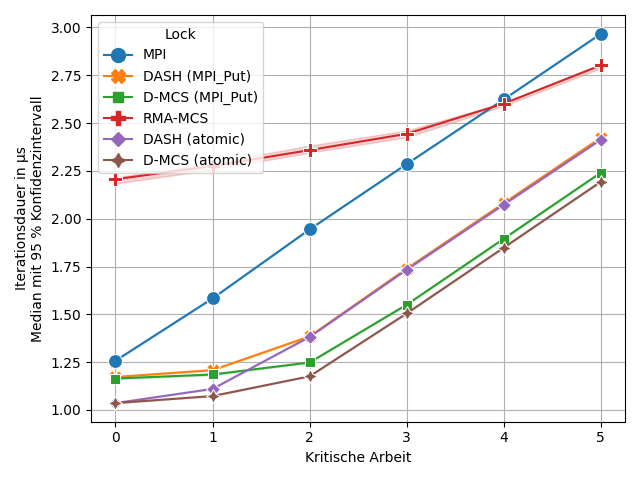
\includegraphics[width=\textwidth]{benchmarks/intelmpi/baseline-opt/CCWB-processes=28-latency}
        \caption{28 Prozesse}
        \label{ben:baseline_opt_ccwb_28_latency}
    \end{subfigure}
    \begin{subfigure}{.5\textwidth}
        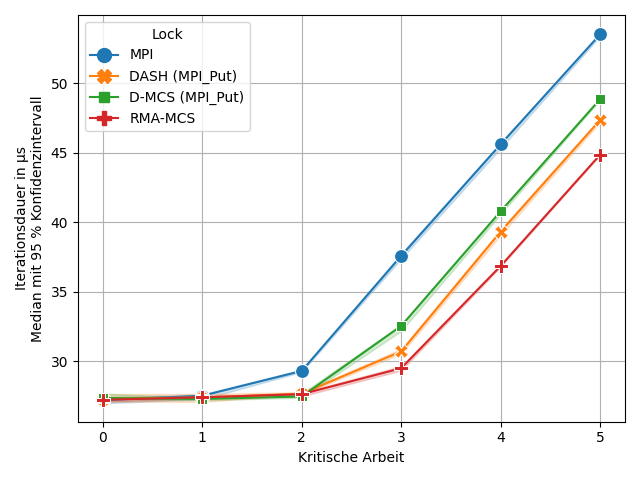
\includegraphics[width=\textwidth]{benchmarks/intelmpi/baseline-opt/CCWB-processes=112-latency}
        \caption{112 Prozesse}
        \label{ben:baseline_opt_ccwb_112_latency}
    \end{subfigure}
    \caption{CCWB der Basislocks-Optimierungen: Iterationsdauer in \textmu{s}}
    \label{ben:baseline_opt_ccwb}
\end{benchmark}

\clearpage

\autoref{ben:baseline_opt_ccwb} zeigt schließlich die optimierten Varianten von D-MCS und \texttt{dash::Mutex} noch einmal im Vergleich miteinander
und zusätzlich im Vergleich zu dem Intel-MPI-Lock und RMA-MCS auf einem und vier Rechenknoten.
In \autoref{ben:baseline_opt_ccwb_28_latency} sieht man,
dass bei einem Knoten der optimierte D-MCS,
also \gls{rma},
schneller ist.
\autoref{ben:baseline_opt_ccwb_112_latency} zeigt,
dass bei mehreren Knoten hingegen der optimierte \texttt{dash::Mutex},
also Punkt-zu-Punkt-Kommunikation,
schneller ist.
Beide optimierte Varianten schlagen den Intel-MPI-Lock,
welcher zuvor auf einem Rechenknoten am schnellsten war,
aber trotz aller Optimierungen erreicht bei mehreren Rechenknoten weiterhin keiner der Locks die Geschwindigkeit von RMA-MCS.
Das zeigt deutlich das enorme Potenzial der Portierung von \gls{numa}-Locks auf verteilten Speicher.

\chapter{Portierung von NUMA-Locks auf verteilten Speicher}
\label{ch:portierung}

Es gibt einige Locks für Systeme mit gemeinsamem Speicher,
die die Unterschiede zwischen Zugriffen auf lokalen und entfernten Speicher bei \gls{numa} berücksichtigen
und Fairness opfern,
um höhere Geschwindigkeiten zu erreichen.
Obwohl die Geschwindigkeitsunterschiede von Speicherzugriffen in verteilten Systemen noch deutlich ausgeprägter sind,
wird diese Technik dort kaum genutzt.
Dabei ähneln sich Speicherzugriffe auf gemeinsamem Speicher und \gls{rma} auf verteilten Systemen stark.
In diesem Kapitel werden daher einige \gls{numa}-Locks untersucht
und wenn möglich auf verteilten Speicher portiert.

\section{Delegierende Locks}
\label{sec:delegation_locks}

Neben klassischen Locks,
die in \autoref{sec:synchronisierung_in_parallelen_programmen} beschrieben wurden,
gibt es bei Systemen mit gemeinsamem Speicher das Konzept von delegierenden Locks,
welche zum Teil auch \gls{numa} berücksichtigen \cite{OyamaAlg} \cite{FlatCombining} \cite{P-Sim} \cite{H-Sync} \cite{RCL} \cite{shared-mem-delegation} \cite{SANL} \cite{DYLOCK}.
Die Idee dabei ist,
dass ein oder mehrere Prozesse als Server agieren
und kritische Abschnitte für alle anderen Client-Prozesse ausführen.
Client-Prozesse schicken dafür Anfragen an den Server,
in denen der auszuführende kritische Abschnitt,
sowie die notwendigen Parameter enthalten sind
und warten auf eine Antwort des Servers,
die zeigt,
dass der kritische Abschnitt ausgeführt wurde.

Unterschieden wird dabei zwischen statischen und dynamischen Locks,
je nachdem,
ob ein oder mehrere fest bestimmte Prozesse als Server dienen,
oder jeder Prozess dynamisch für eine gewisse Zeit zu einem Server werden kann.

Delegierende Locks haben in Systemen mit gemeinsamem Speicher den großen Vorteil,
dass die Daten,
die durch den Lock geschützt werden
und auf die im kritischen Abschnitt zugegriffen wird,
immer von demselben Prozess (dem Server-Prozess) verwendet werden.
Damit liegen sie dort typischerweise in lokalen \gls{Zwischenspeicher}n vor,
wodurch besonders schnell auf sie zugegriffen werden kann.

Ein Nachteil von delegierenden Locks ist allerdings,
dass sie nicht dieselbe Programmierschnittstelle nutzen können
wie klassische Locks,
weil sie Zugriff auf alle Parameter des kritischen Abschnitts benötigen
und der kritische Abschnitt selbst eine eigene Funktion sein muss,
damit der Server-Prozess diese direkt aufrufen kann.
Ein Programm von klassischen Locks auf delegierende Locks umzustellen,
kann daher sehr aufwendig sein.

Bei verteiltem Speicher besteht darüber hinaus das Problem,
dass Prozesse im kritischen Abschnitt auch auf private Daten zugreifen können,
die nicht über ein \gls{Fenster} veröffentlicht wurden.
In so einem Fall ist es für einen anderen Prozess gar nicht möglich,
den kritischen Abschnitt auszuführen.
Delegierende Locks eignen sich daher nicht für eine Portierung auf verteilten Speicher.
Außerdem kommt der Hauptvorteil von delegierenden Locks,
dass die Daten des kritischen Abschnitts meist schon im \gls{Zwischenspeicher} des Server-Prozesses liegen,
bei verteiltem Speicher nicht zum Tragen,
da in \gls{mpi} die Daten von entfernen Prozessen nicht automatisch zwischengespeichert werden.

Das Konzept der Delegierung an einen Server-Prozess passt allerdings sehr gut zu \gls{message passing}
und die hier beschriebenen Probleme lassen sich leicht vermeiden,
wenn ein Programm speziell dafür entwickelt wird.
Daher eignet sich dieses Konzept möglicherweise,
um parallele Datenstrukturen,
z.~B. Warteschlangen (engl. \textit{Queues}),
für verteilte Systeme zu entwickeln.

\section{RH-Lock}
\label{sec:rh-lock}

Der RH-Lock \cite{RH-Lock} ist der erste bekannte Lock
der \gls{numa} berücksichtigt,
um eine bessere Performance zu erzielen.
Er besteht aus einem \gls{tts}-Lock \cite{TTS-Lock} mit exponentiellem Backoff \cite{backoff} (siehe \autoref{sec:spin_locks}) pro \gls{numa}-Knoten.
Da der RH-Lock nur zwei \gls{numa}-Knoten unterstützt,
sind es also immer zwei \gls{tts}-Locks.

Statt einer \textit{Test-and-Set}-Operation,
nutzen die \gls{tts}-Locks für lokale Akquisitionen keine \gls{tas}-,
sondern eine \textit{swap}-Operation,
da der Lock-Status nicht nur die Werte \enquote{FREE} und \enquote{ACQUIRED} annehmen kann.
Wenn der Lock nicht verfügbar ist,
enthält der Lock-Status stattdessen die eindeutige ID des Prozesses,
der zuletzt mit einer \textit{swap}-Operation versucht hat,
den Lock zu akquirieren,
oder den Status \enquote{REMOTE},
wenn zuletzt ein Prozess des anderen \gls{numa}-Knotens den Lock erfolgreich akquiriert hat.

Durch die IDs hat ein Prozess die Möglichkeit,
den Lock mit einer \gls{cas}-Operation nur dann global freizugeben,
wenn der Status immer noch seine ID enthält.
Wenn diese \gls{cas}-Operation fehlschlägt,
muss es innerhalb seines \gls{numa}-Knotens einen anderen Prozess geben,
der auf den Lock wartet.
In diesem Fall wird der Lock mit dem Status \enquote{L\_FREE} nur lokal,
also für Prozesse im selben \gls{numa}-Knoten freigeben.

Liest ein Prozess den Status \enquote{REMOTE},
weiß er,
dass er die Speicheradresse des \gls{tts}-Locks
des jeweils anderen \gls{numa}-Knotens
für die Akquisition
nutzen muss.
Durch die \textit{swap}-Operation
sieht nur der erste Prozess eines \gls{numa}-Knotens den \enquote{REMOTE} Status.
Alle weiteren Prozesse sehen die ID ihres Vorgängers
und warten auf den lokalen \gls{tts}-Lock.

Um einen entfernten \gls{tts}-Lock zu akquirieren,
prüft ein Prozess,
anders als bei seinem lokalen \gls{tts}-Lock,
nicht zuerst mit einer Lese-Operation,
ob der Lock frei ist.
Der Lock funktioniert in diesem Fall also eher wie ein \gls{tas}-Lock (vgl. \autoref{fig:tas_code}) mit Backoff.
Dadurch,
dass entfernte Zugriffe langsamer sind,
hätte ein entfernter Prozess sonst kaum eine Chance,
den Lock zu akquirieren,
da er deutlich länger braucht,
um darauf zu reagieren,
dass der Lock frei ist.
Stattdessen versucht ein Prozess immer direkt mit einer \gls{cas}-Operation,
den entfernten Lock zu akquirieren.
Hierbei wird \gls{cas},
statt \textit{swap} genutzt,
da der entfernte Lock nur akquiriert werden soll,
wenn er den Status \enquote{FREE},
nicht aber z.~B. den Status \enquote{L\_FREE} hat.

Um \gls{Verhungern} zu vermeiden,
% also dass immer wieder Prozesse desselben \gls{numa}-Knotens den Lock akquirieren
% und die anderen Prozesse für immer warten,
setzt der RH-Lock einen Zufallszahlengenerator ein
und gibt mit konfigurierbarer Wahrscheinlichkeit den Lock global frei,
selbst wenn es einen lokalen wartenden Prozess gibt,
sodass alle Prozesse die Möglichkeit haben,
den Lock zu akquirieren.

\clearpage

\subsection{Portierung und Optimierung des RH-Locks}

Das größte Problem des RH-Locks für eine Portierung auf verteilten Speicher ist,
dass der Lock nur zwei \gls{numa}-Knoten unterstützt.
Es ist aber eher selten,
dass ein verteiltes System aus nur zwei Knoten besteht.
Dieses Problem lässt sich z.~B. beheben,
indem man den \enquote{REMOTE} Status erweitert
und dort zusätzlich die ID des entfernten Prozesses codiert,
in dessen Speicher der \gls{tts}-Lock ist.
Für die Portierung werden hierfür negative Zahlen verwendet ($-id - 1$ um die ID 0 zu unterstützen),
da Prozess IDs typischerweise positiv sind.
Somit signalisiert eine positive Zahl,
dass der Prozess lokal warten muss
und eine negative Zahl,
dass der Prozess auf den \gls{tts}-Lock
im Speicher des entfernten Prozesses mit der zugehörigen positiven ID warten muss.

Bei mehr als zwei Knoten kann es nun allerdings passieren,
dass ein Prozess auf Knoten $a$ einen \enquote{REMOTE} Wert liest,
der ihn auf Knoten $b$ verweist,
obwohl Knoten $b$ den Lock gar nicht mehr hat,
da inzwischen ein Prozess von Knoten $c$ den Lock akquiriert hat.
Daher kann ein Prozess nicht mehr einfach darauf warten,
dass der \gls{tts}-Lock des anderen Knotens frei wird,
sondern muss auch dort prüfen,
ob es sich um einen \enquote{REMOTE} Wert handelt,
der ihn weiter verweist.
Bei einem freien RH-Lock muss ein Prozess so im schlimmsten Fall jeden anderen \gls{tts}-Lock fragen,
bis er den richtigen findet.
Dieser Overhead steigt demnach linear mit der Anzahl der beteiligten Knoten.

Beim RH-Lock gehen die meisten Speicherzugriffe auf den lokalen \gls{tts}-Lock des \gls{numa}-Knotens,
was gut ist,
da lokale Zugriffe schneller als entfernte sind.
Dabei handelt es sich vor allem um die Lese-Operation,
mit der ermittelt wird,
ob der Lock frei ist.
Da es sich um einen lokalen Zugriff handelt,
kann genau diese Operation ohne \gls{rma} mit einem schnelleren direkten Speicherzugriff implementiert werden,
wenn für die lokale Kommunikation ein \gls{Fenster} auf den gemeinsamen Speicher erstellt wurde
(vgl. \autoref{sec:mpi_shared_mem}).
Dabei ist zu beachten,
dass in der Warteschleife \texttt{MPI\_Iprobe} aufgerufen wird,
um Programmfortschritt zu garantieren (vgl. \autoref{sec:mpi_fortschritt}).

\subsection{Evaluation des RH-Locks}

Da die Warteschleife einen Aufruf von \texttt{MPI\_Iprobe} enthalten muss,
um Programmfortschritt zu garantieren,
ist sie deutlich langsamer
als eine leere Warteschleife,
wie sie in \cite{RH-Lock} genutzt wird.
Außerdem ist die Latenz von Zugriffen auf entfernten Speicher
in einem verteilten System deutlich höher
als in einem System mit gemeinsamem \gls{numa}-Speicher,
da der Zugriff über das Netzwerk gehen muss.
Allein aus diesem Grund ist die Frequenz,
mit der versucht wird,
einen entfernten \gls{tts}-Lock zu akquirieren,
deutlich geringer.
Aus diesen beiden Gründen können nicht einfach dieselben Werte für Backoff (vgl. \autoref{sec:spin_locks}) verwendet werden
wie in \cite{RH-Lock}.

Durch die hohe Latenz von entfernten Speicherzugriffen,
ist die Frequenz dieser Zugriffe während des Wartens auf einen entfernten \gls{tts}-Lock bereits so niedrig,
dass zusätzlicher Backoff keine Verbesserung bringt,
sondern entfernte Prozesse nur unfair benachteiligt.
Der initiale und maximale Backoff für das entfernte Akquirieren werden daher in der Evaluation auf 0 gesetzt,
wodurch der Backoff deaktiviert wird.

Für Zugriffe auf den lokalen \gls{tts}-Lock hingegen ist Backoff weiterhin sinnvoll.
Durch die Verwendung von \texttt{MPI\_Iprobe}
sind die optimalen Werte aber deutlich geringer
als in \cite{RH-Lock}.
Als maximaler Backoff werden lokal 16, 32 und 64 Iterationen evaluiert,
da ungefähr bei 32 Backoff-Iterationen ein lokales Optimum
bei einer durchschnittlichen Wartezeit von 1~\textmu{s} im \gls{wbab} liegt.
Da diese Maximalwerte so klein sind,
wird als Minimalwert immer 1 verwendet.
So erreicht ein Prozess spätestens nach dem 7. Zugriff auf den \gls{tts}-Lock die maximale Wartezeit von $2^6 = 64$ Iterationen.

Wie bereits in \autoref{sec:spin_locks} erläutert,
hängt die optimale Backoff-Konfiguration von der Geschwindigkeit des verwendeten Systems,
aber auch von dem konkreten Szenario (Länge des kritischen Abschnitts, Anzahl der Prozesse) ab.
Es ist also möglich,
dass in manchen Szenarien eine andere Konfiguration besser wäre.
Die Optimierung auf eine durchschnittliche Wartezeit von 1~\textmu{s} im \gls{wbab} ist zwar willkürlich,
liefert aber zumindest deutlich bessere Ergebnisse
als eine einfache Wiederverwendung der Konfiguration aus \cite{RH-Lock}.

Neben dem Backoff ist beim RH-Lock auch die Fairness konfigurierbar.
Hier muss eingestellt werden,
mit welcher Wahrscheinlichkeit trotz lokalen Nachfolgers der Lock global freigegeben wird.
In dieser Arbeit werden für einen maximalen lokalen Backoff von 32,
wie in \cite{RH-Lock} die Fairnessfaktoren 1, 2 \& 100 evaluiert.
D.~h. der Lock wird bei einem lokalen Nachfolger trotzdem mit einer Wahrscheinlichkeit von $1$, $\frac{1}{2}$ oder $\frac{1}{100}$ global freigegeben.
Bei einem maximalem lokalen Backoff von 16 und 64 ist der RH-Lock in dieser Arbeit immer maximal fair (also mit einem Fairnessfaktor von 1) eingestellt.

\begin{benchmark}[h]
    \begin{subfigure}{.5\textwidth}
        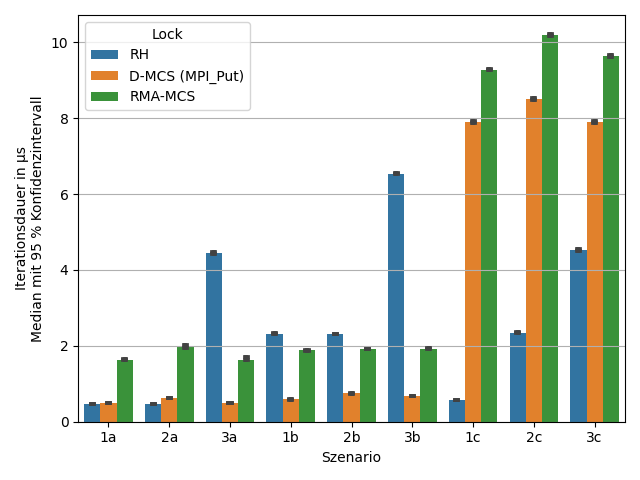
\includegraphics[width=\textwidth]{benchmarks/intelmpi/rh/UPB-lock_count=1000-latency}
        \caption{Iterationsdauer in \textmu{s}}
        \label{ben:rh_upb_latency}
    \end{subfigure}
    \begin{subfigure}{.5\textwidth}
        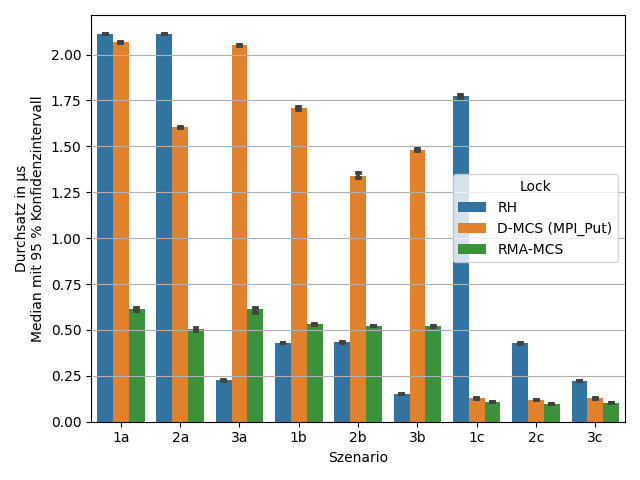
\includegraphics[width=\textwidth]{benchmarks/intelmpi/rh/UPB-lock_count=1000-throughput}
        \caption{Durchsatz in Mio/s}
        \label{ben:rh_upb_throughput}
    \end{subfigure}
    \caption{UPB des RH-Locks}
    \label{ben:rh_upb}
\end{benchmark}

\autoref{ben:rh_upb_latency} zeigt,
wie lange es dauert,
einen freien RH-Lock zu akquirieren,
im Vergleich zum optimierten D-MCS-Lock aus \autoref{sec:optimierung_dmcs} und RMA-MCS.
Die Backoff- und Fairness-Konfiguration spielt für diesen Benchmark keine Rolle,
da alle Locks frei sind,
somit wird hier nur ein RH-Lock gezeigt.
Anders als bei den anderen \gls{upb}-Evaluationen,
sind hier alle neun Szenarien (vgl. \autoref{tab:upb_szenarien}) separat aufgeführt.
Beim RH-Lock macht es nämlich einen Unterschied,
welcher Prozess den Lock als Letztes besaß.

Während es bei den optimierten D-MCS- und RMA-MCS-Locks vor allem entscheidend ist,
wie weit der akquirierende Prozess vom Hauptprozess entfernt ist,
also ob es ein a-, b- oder c-Szenario ist,
ist es beim RH-Lock vor allem wichtig,
ob der Vorgängerprozess auf demselben Knoten lief,
also ob es ein 1er, 2er oder 3er-Szenario ist.
Das liegt daran,
dass es beim RH-Lock keinen globalen Hauptprozess gibt.
Alle Rechenknoten sind beim RH-Lock äquivalent.
Es gibt allerdings auf jedem Rechenknoten einen lokalen Hauptprozess,
in dessen Speicher sich der \gls{tts}-Lock befindet.

\clearpage

Überraschenderweise lässt sich ein RH-Lock schneller durch einen lokalen Hauptprozess akquirieren.
\autoref{ben:rh_upb} zeigt deutlich,
dass der RH-Lock in den b-Szenarien (Prozess ist kein Hauptprozess) deutlich langsamer ist
als in den a-Szenarien (Prozess ist ein Hauptprozess).
In den c-Szenarien ist das Bild gemischt.
Die c-Szenarien zeigen die Performance,
wenn der akquirierende Prozess nicht auf dem Hauptknoten läuft.
D-MCS und RMA-MCS sind hier deutlich langsamer als in den anderen Szenarien,
da sie entferne Zugriffe auf den Hauptknoten benötigen.
Beim RH-Lock gibt es aber keinen Hauptknoten,
sodass er sich in c-Szenarien genauso verhält
wie in den anderen.
Das gemischte Bild entsteht dadurch,
dass der akquirierende Prozess in Szenario 1c und 3c ein lokaler Hauptprozess ist,
in 2c aber nicht.
Daher ist die Performance des RH-Locks in Szenario 1c identisch zu der in 1a,
in 2c identisch zu der in 2b
und in 3c identisch zu der in 3a.

% Tatsächlich sieht man,
% dass auch D-MCS und RMA-MCS in Szenario 2c etwas langsamer sind
% als in 1c und 3c.
% Bei RMA-MCS könnte das daran liegen,
% dass auch dieser lokale Hauptprozesse nutzt.
% Bei D-MCS ist das aber nicht der Fall.
% Hier greift der akquirierende Prozess in allen drei c-Szenarien nur auf seinen eigenen
% und den entfernten Speicher des globalen Hauptprozesses zu.
% Warum die Performance von D-MCS in Szenario 2c schlechter ist,
% ist also nicht klar.

\begin{benchmark}[h]
    \begin{subfigure}{.5\textwidth}
        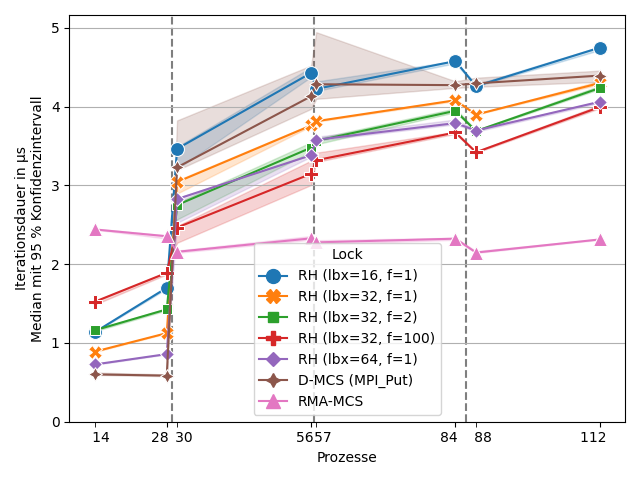
\includegraphics[width=\textwidth]{benchmarks/intelmpi/rh/ECSB-latency}
        \caption{Iterationsdauer in \textmu{s}}
        \label{ben:rh_ecsb_latency}
    \end{subfigure}
    \begin{subfigure}{.5\textwidth}
        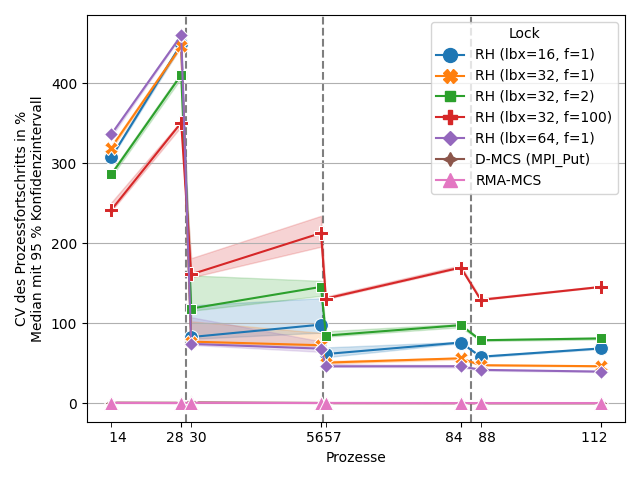
\includegraphics[width=\textwidth]{benchmarks/intelmpi/rh/ECSB-fairness}
        \caption{Fairness: CV des Fortschritts in \%}
        \label{ben:rh_ecsb_fairness}
    \end{subfigure}
    \caption{ECSB des RH-Locks}
    \label{ben:rh_ecsb}
\end{benchmark}

\autoref{ben:rh_ecsb} zeigt den \gls{ecsb} für die verschiedenen Konfigurationen des RH-Locks,
den D-MCS und RMA-MCS.
Dabei steht \enquote{lbx} für \enquote{lokales Backoff-Maximum} und \enquote{f} für \enquote{Fairnessfaktor}.
In \autoref{ben:rh_ecsb_latency} sieht man,
dass bei mehreren Rechenknoten alle RH-Locks (außer mit lbx=16) schneller sind
als der D-MCS-Lock.
Dieser Vorteil wird aber mit erheblichen Fairnessproblemen erkauft,
wie \autoref{ben:rh_ecsb_fairness} zeigt.
Während D-MCS und RMA-MCS sehr fair sind (ohne erkennbare Abweichung von 0~\%),
haben alle RH-Locks extrem schlechte Fairnesswerte,
auf einem Rechenknoten sogar einen Variationskoeffizienten von bis zu 460~\%.
Bei mehr Rechenknoten wird es zwar etwas besser,
der fairste RH-Lock fällt bei 112 Prozessen auf einen Variationskoeffizienten von knapp unter 40~\%,
aber sie bleiben ziemlich unfair.
Da im \gls{ecsb} Prozesse außerhalb des kritischen Abschnitts nichts tun müssen,
kann derselbe Prozess den Lock immer wieder akquirieren
und so anderen Prozessen zuvorkommen.
Daher ist die Fairness in diesem Benchmark besonders schlecht.

\autoref{ben:rh_ecsb_fairness} zeigt auch,
dass die Fairness auf mehreren Rechenknoten noch weiter abnimmt,
wenn andere Werte für den Fairnessfaktor verwendet werden (2 und 100).
Die Geschwindigkeit in \autoref{ben:rh_ecsb_latency} nimmt dafür weiter zu.
Man hat also hier die Möglichkeit,
noch mehr Fairness für Geschwindigkeit zu opfern.
Trotzdem kommt der RH-Lock mit keiner der Konfigurationen an die Geschwindigkeit von RMA-MCS heran,
welcher obendrein auch noch sehr fair ist.
Dieser hat allerdings in diesem Vergleich
die mit Abstand schlechteste Performance
bei nur einem Rechenknoten (auf 14 und 28 Prozessen).

\begin{benchmark}[h]
    \begin{subfigure}{.5\textwidth}
        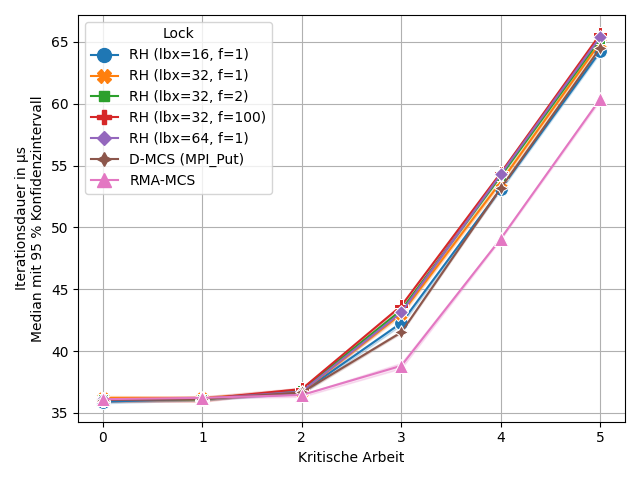
\includegraphics[width=\textwidth]{benchmarks/intelmpi/rh/CCWB-processes=112-latency}
        \caption{Iterationsdauer in \textmu{s}}
        \label{ben:rh_ccwb_112_latency}
    \end{subfigure}
    \begin{subfigure}{.5\textwidth}
        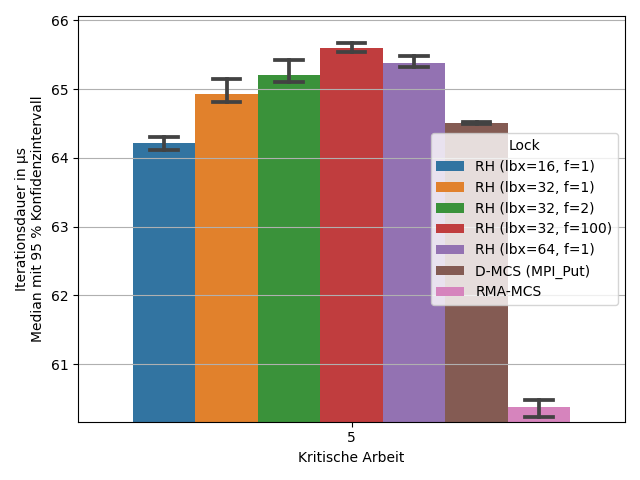
\includegraphics[width=\textwidth]{benchmarks/intelmpi/rh/CCWB-processes=112-latency-max}
        \caption{Iterationsdauer in \textmu{s}}
        \label{ben:rh_ccwb_112_latency_max}
    \end{subfigure}
    \begin{subfigure}{.5\textwidth}
        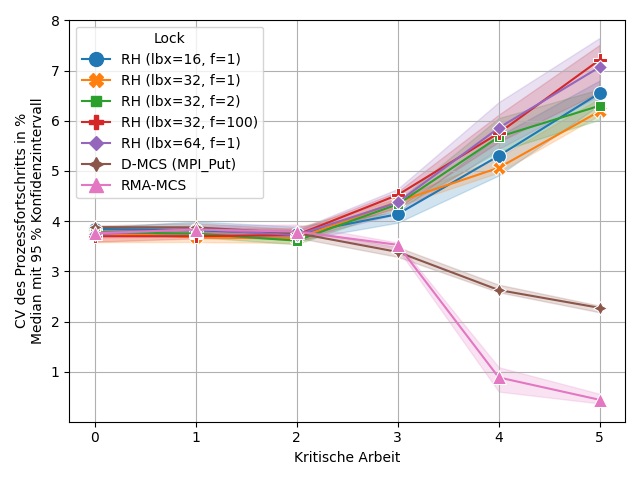
\includegraphics[width=\textwidth]{benchmarks/intelmpi/rh/CCWB-processes=112-fairness}
        \caption{Fairness: CV des Fortschritts in \%}
        \label{ben:rh_ccwb_112_fairness}
    \end{subfigure}
    \begin{subfigure}{.5\textwidth}
        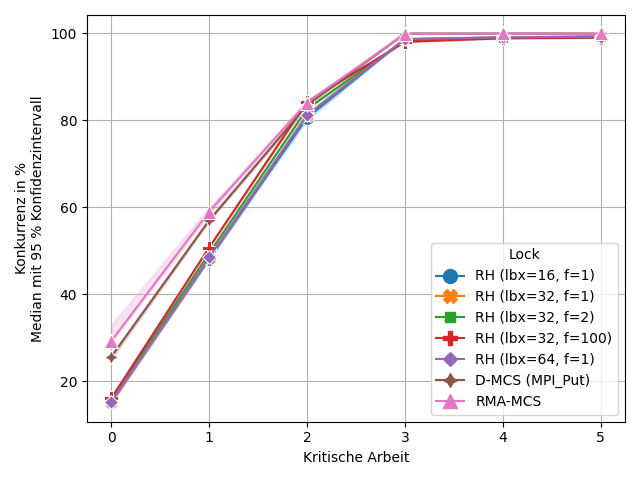
\includegraphics[width=\textwidth]{benchmarks/intelmpi/rh/CCWB-processes=112-contention}
        \caption{Konkurrenz in \%}
        \label{ben:rh_ccwb_112_contention}
    \end{subfigure}
    \caption{CCWB des RH-Locks mit 112 Prozessen}
    \label{ben:rh_ccwb_112}
\end{benchmark}

Auch beim \gls{ccwb} sieht man in \autoref{ben:rh_ccwb_112_fairness},
dass der RH-Lock deutlich unfairer ist
als D-MCS und RMA-MCS.
Vor dem Equilibrium sind alle Locks gleich fair.
Während bei D-MCS und RMA-MCS die Fairness ab dem Equilibrium besser wird,
da Prozesse sich bei einer \gls{Konkurrenz} von 100~\% in eine Warteschlange mit beschränkter Fairness einreihen müssen,
wird die Fairness des RH-Locks in allen Konfigurationen immer schlechter.
Die Fairness ist aber um ein Vielfaches besser
als im \gls{ecsb},
da der \gls{ccwb} ein deutlich realistischeres Szenario implementiert,
bei dem Prozesse auch außerhalb des kritischen Abschnitts Arbeit ausführen.

Die bessere Fairness bringt aber leider auch eine schlechtere Geschwindigkeit mit sich.
Im Gegensatz zum \gls{ecsb} ist der RH-Lock hier nur mit einem \enquote{lbx} von 16 schneller
als der D-MCS-Lock.
Und das auch nur bei einer kritischen Arbeit von 4 und 5.
Beim \gls{ecsb} war es genau anders herum:
Dort war der RH-Lock nur mit einem \enquote{lbx} von 16 langsamer als der D-MCS-Lock.
Da die Locks in \autoref{ben:rh_ccwb_112_latency} so dicht beieinanderliegen,
dass sie schwer zu unterscheiden sind,
zeigt \autoref{ben:rh_ccwb_112_latency_max} eine Nahaufnahme der Performance bei einer kritischen Arbeit von 5.
Diese Nahaufnahme zeigt überraschenderweise,
dass ein höherer Fairnessfaktor im \gls{ccwb} zu einem langsameren Lock führt.
Auch das war im \gls{ecsb} genau umgekehrt.
Die Idee des Fairnessfaktors ist es eigentlich,
Fairness zu opfern,
um die Geschwindigkeit zu verbessern.
Der \gls{ccwb} zeigt aber,
dass in einem realistischen Szenario durch einen höheren Fairnessfaktor sowohl Fairness
als auch Geschwindigkeit geopfert werden.

Der Grund hierfür ist wahrscheinlich,
dass die Lock-Freigabe aus einer zusätzlichen \gls{cas}-Operation besteht,
wenn sich der Prozess unfair verhält,
also den Lock nur lokal freigibt.
Der Status darf nur auf \enquote{L\_FREE} gesetzt werden,
wenn es einen lokalen Nachfolger gibt.
Sonst könnte es zu einem Deadlock kommen.
Daher wird bei der unfairen Freigabe der Status erst gesetzt,
wenn die \gls{cas}-Operation fehlschlägt,
die den Lock global freigeben würde.
Die zusätzliche \gls{cas}-Operation liegt auf dem kritischen Pfad
und schlägt bei einer kritischen Arbeit von 5 immer fehl,
da die \gls{Konkurrenz} bei 100~\% liegt (vgl. \autoref{ben:rh_ccwb_112_contention}).
Die faire Freigabe hingegen besteht nur aus einer Operation,
die den Status immer auf \enquote{FREE} setzt.

Obwohl die zusätzliche \gls{cas}-Operation auf lokalen Speicher zugreift,
kann sie nicht mit C++ \texttt{std::atomic} implementiert werden,
da auf dieselbe Speicheradresse auch entfernt zugegriffen wird.
Es muss also ein langsamer \gls{rma}-Zugriff verwendet werden.
Auf gemeinsamem Speicher wird die zusätzliche \gls{cas}-Operation dadurch ausgeglichen,
dass durch eine lokale Lockübergabe die Daten,
auf die der Nachfolgerprozess im kritischen Abschnitt zugreift,
bereits im \gls{Zwischenspeicher} vorliegen.
Bei verteiltem Speicher gibt es allerdings keine \gls{Zwischenspeicher} für entfernten Speicher,
sodass dieser Vorteil hier nicht zum tragen kommt.

\begin{benchmark}[h]
    \begin{subfigure}{.5\textwidth}
        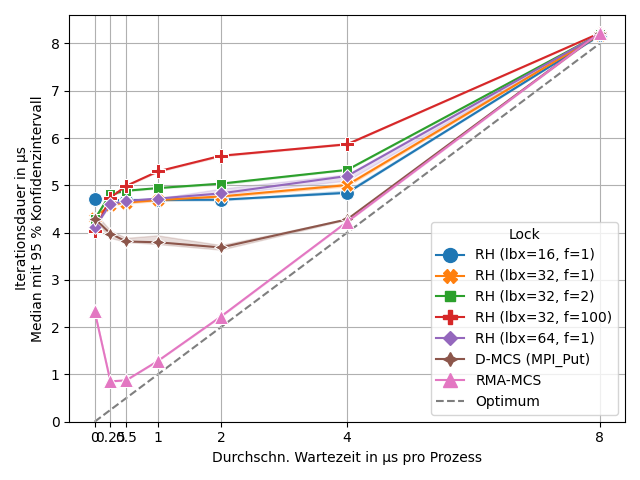
\includegraphics[width=\textwidth]{benchmarks/intelmpi/rh/WBAB-processes=112,mpi_progress=1-latency}
        \caption{Iterationsdauer in \textmu{s}}
        \label{ben:rh_wbab_112_latency}
    \end{subfigure}
    \begin{subfigure}{.5\textwidth}
        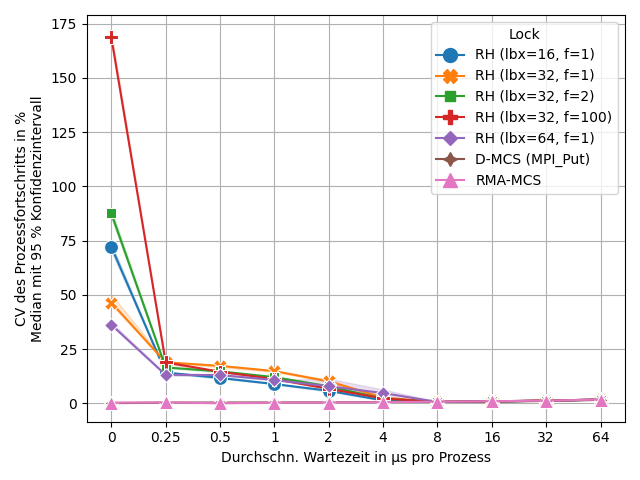
\includegraphics[width=\textwidth]{benchmarks/intelmpi/rh/WBAB-processes=112,mpi_progress=1-fairness}
        \caption{Fairness: CV des Fortschritts in \%}
        \label{ben:rh_wbab_112_fairness}
    \end{subfigure}
    \begin{subfigure}{.5\textwidth}
        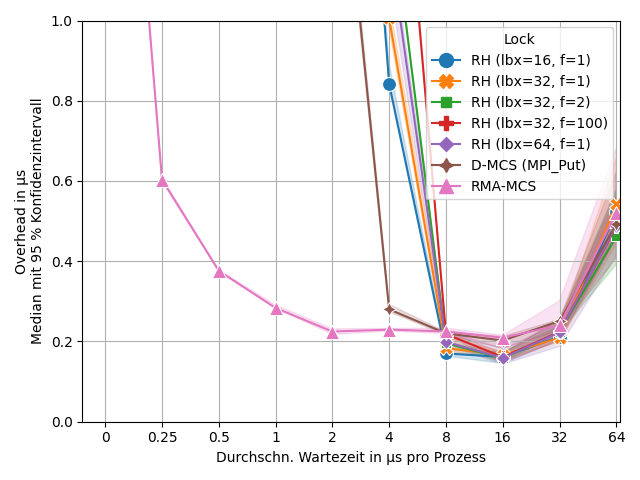
\includegraphics[width=\textwidth]{benchmarks/intelmpi/rh/WBAB-processes=112,mpi_progress=1-overhead}
        \caption{Overhead in \textmu{s}}
        \label{ben:rh_wbab_112_overhead}
    \end{subfigure}
    \begin{subfigure}{.5\textwidth}
        \includegraphics[width=\textwidth]{benchmarks/intelmpi/rh/WBAB-processes=112,mpi_progress=1-contention}
        \caption{Konkurrenz in \%}
        \label{ben:rh_wbab_112_contention}
    \end{subfigure}
    \caption{WBAB des RH-Locks mit 112 Prozessen}
    \label{ben:rh_wbab_112}
\end{benchmark}

\autoref{ben:rh_wbab_112} zeigt die Ergebnisse des RH-Locks im \gls{wbab}.
Genau wie im \gls{ccwb} führt auch beim \gls{wbab} ein höherer Fairnessfaktor
zu einem langsameren Lock.
Bei der Geschwindigkeit in \autoref{ben:rh_wbab_112_latency} erreicht keiner der RH-Locks mehr die Performance von D-MCS,
sobald Prozesse außerhalb des kritischen Abschnitts warten.
Dafür zeigt \autoref{ben:rh_wbab_112_overhead} aber,
dass bei geringer \gls{Konkurrenz}
(Wartezeit von 8~\textmu{s} bis 32~\textmu{s})
der RH-Lock in allen Konfigurationen schneller ist
als D-MCS und sogar RMA-MCS.
Das passt auch zu den Ergebnissen aus \autoref{ben:rh_upb},
nach denen ein freier RH-Lock schneller als D-MCS und RMA-MCS akquiriert werden kann,
wenn der Prozess nicht auf dem Hauptknoten läuft.
Der RH-Lock hat hier den Vorteil,
dass keine MCS-Warteschlangen initialisiert werden müssen.

In \autoref{ben:rh_wbab_112_fairness} sieht man noch einmal die extreme Unfairness des RH-Locks,
wenn Prozesse keine Wartezeit außerhalb des kritischen Abschnitts haben,
die auch der \gls{ecsb} gezeigt hat.
Diese wird bereits bei geringer Wartezeit deutlich besser,
bleibt aber suboptimal,
bis die \gls{Konkurrenz} bei einer Wartezeit von 8~\textmu{s} stark abfällt
(vgl. \autoref{ben:rh_wbab_112_contention}).
Ab diesem Punkt muss kein Prozess mehr lange auf den Lock warten,
wodurch der RH-Lock auch nicht mehr unfair sein kann.

Bei der \gls{Konkurrenz} in \autoref{ben:rh_wbab_112_contention} ist sehr auffällig,
dass bei keinem RH-Lock je eine \gls{Konkurrenz} von deutlich über 90~\% erreicht wird.
Ohne Wartezeit ist sie sogar noch geringer.
Das stützt die Hypothese,
dass ohne unkritische Arbeit häufig derselbe Prozess den Lock immer wieder akquiriert und so anderen Prozessen zuvorkommt.
Dass auch mit unkritischer Arbeit etwa jeder zehnte Prozess einen freien Lock beobachtet,
ist so allerdings nicht zu erklären.

Zusammenfassend lässt sich sagen,
dass der RH-Lock zwar bei geringer \gls{Konkurrenz} eine gute Performance hat,
sobald die \gls{Konkurrenz} jedoch steigt,
hat er enorme Fairnessprobleme
und ist kaum schneller als ein optimierter MCS-Lock.
Außerdem muss der RH-Lock je nach System
und erwarteter Konkurrenzsituation anders konfiguriert werden,
um eine gute Performance zu erreichen,
was zusätzlichen Aufwand für den Einsatz bedeutet.

Es könnte aber Fälle geben,
in denen die Eigenschaft,
dass es keinen festen Hauptprozess gibt,
sondern der Lock immer auf dem Rechenknoten lokal ist,
auf dem er zuletzt akquiriert wurde,
große Vorteile bringt.
Dadurch muss nicht im Voraus ein Hauptprozess definiert werden
und wenn besonders Prozesse,
die auf demselben Knoten laufen,
häufig gleichzeitig den kritischen Abschnitt betreten möchten,
kann so mit Sicherheit eine gute Performance erreicht werden.
So ein Szenario ist in den Benchmarks dieser Arbeit zwar nicht enthalten,
aber durchaus denkbar.
Möglicherweise lässt sich der Ansatz eines wechselnden Hauptprozesses in einem zukünftigen Lock
mit einer besseren Fairness realisieren.

\section{HCLH-Lock}
\label{sec:hclh-lock}

Der HCLH-Lock \cite{HCLH-Lock} basiert auf dem CLH-Lock,
welcher unabhängig von Craig \cite{C-Lock} und Landin und Hagersten \cite{LH-Lock} entwickelt wurde
und dem MCS-Lock sehr ähnelt.

\subsection{CLH-Lock}

\begin{figure}[h]
    \begin{subfigure}[b]{.5\textwidth}
        \centering
        \begin{tabular}{c}\begin{lstlisting}
struct node { atomic<bool> locked; };
node* myreq; // Pro Prozess
node* watch; // Pro Prozess
atomic<node*> tail; // Pro Lock

void initialize() {
  myreq = new node();
  if (hauptprozess)
    tail.store(new node());
}
        \end{lstlisting}\end{tabular}
        \caption{Felder und Initialisierung}
        \label{fig:clh_init}
    \end{subfigure}
    \begin{subfigure}[b]{.5\textwidth}
        \centering
        \begin{tabular}{c}\begin{lstlisting}
void acquire() {
  myreq->locked.store(true);
  watch = tail.exchange(myreq);
  while (watch->locked.load());
}

void release() {
  myreq->locked.store(false);
  myreq = watch;
}
        \end{lstlisting}\end{tabular}
        \caption{Akquirieren und Freigeben des Locks}
        \label{fig:clh_acq_rel}
    \end{subfigure}
    \caption{CLH-Lock}
    \label{fig:clh_code}
\end{figure}

\autoref{fig:clh_code} zeigt eine C++-Implementierung des CLH-Locks.
Die Felder und Initialisierung des Locks in \autoref{fig:clh_init} sind dabei leicht vereinfacht.
Die Warteschlangenknoten (engl. \textit{node}) enthalten im Gegensatz zum MCS-Lock nur ein \texttt{locked}-\textit{Flag}
und keinen Zeiger auf den Nachfolger.
Jeder Prozess hat in seinem privaten Speicher zwei Zeiger:
\texttt{myreq} steht für \enquote{Meine Anfrage} (engl. \textit{my request})
und zeigt auf den Knoten,
den der Prozess in die Warteschlange einreihen wird.
Der Zeiger \texttt{watch} (deutsch beobachten) zeigt später auf den Knoten des Vorgängers,
auf den gewartet wird,
initial zeigt er jedoch ins Leere.

Zusätzlich gibt es einmal pro Lock einen Zeiger namens \texttt{tail} (deutsch Ende),
der genau wie beim MCS-Lock auf den letzten Knoten der Warteschlange zeigt.
Auf diesen Zeiger greifen alle Prozesse atomar zu,
er befindet sich daher in öffentlichem Speicher.
Genau wie der \texttt{myreq}-Zeiger jedes Prozesses,
zeigt der \texttt{tail}-Zeiger initial auf einen eigenen Knoten.
Im CLH-Lock gibt es daher immer einen Knoten mehr,
als Prozesse beteiligt sind.
Das \texttt{locked}-\textit{Flag} aller Knoten hat am Anfang den Wert \texttt{false}.

In der \texttt{acquire}-Funktion setzt ein Prozess zunächst das \texttt{locked}-\textit{Flag} seines Knotens auf \texttt{true}.
Dann tauscht er mit einer \texttt{exchange}-Operation (anderer Name für \textit{swap})
den Endknoten der Warteschlange durch seinen eigenen Knoten aus.
Den bisherigen Endknoten merkt er sich mit seinem \texttt{watch}-Zeiger.
Wenn der Prozess der Erste war,
der \texttt{acquire} ausgeführt hat,
dann zeigt \texttt{watch} nun auf den Knoten,
der initial keinem Prozess gehört hat.
Das \texttt{locked}-\textit{Flag} des Knotens hat in diesem Fall immer noch den Initialwert \texttt{false}.
Ansonsten zeigt \texttt{watch} nun auf den Knoten eines Vorgängers,
welcher sein \texttt{locked}-\textit{Flag} vor dem Einreihen in die Warteschlange auf \texttt{true} gesetzt hat.
Nun muss der Prozess also nur noch warten,
bis das \texttt{locked}-\textit{Flag} seines Vorgängers \texttt{false} wird.
Dann kann er den kritischen Abschnitt betreten.

In \texttt{release} setzt ein Prozess einfach das \texttt{locked}-\textit{Flag} seines Knotens auf \texttt{false}
und signalisiert so seinem Nachfolger,
dass er den kritischen Abschnitt betreten kann.
Von nun an kann der Prozess seinen Knoten nicht mehr verwenden,
um sich erneut in die Warteschlange einzureihen,
schließlich weiß er nicht,
wann sein Nachfolger mitbekommt,
dass der Lock frei ist.
Stattdessen nutzt ein Prozess beim nächsten Mal einfach den Knoten,
den er von seinem Vorgänger erhalten hat.
Das erreicht er,
indem er den Zeiger \texttt{myreq} auf denselben Knoten zeigen lässt
wie \texttt{watch}.
Die Knoten werden im CLH-Lock also rotiert,
jeder Prozess erhält jedes Mal den Knoten seines Vorgängers für die nächste Runde.

\subsection{CLH-Lock Variante für NUMA}

Der Hauptunterschied zum MCS-Lock besteht darin,
dass Prozesse im CLH-Lock beim Warten auf ihren Vorgänger einen Speicherbereich beobachten,
der nicht unbedingt in ihrem lokalen Speicher liegt.
Stattdessen beobachten sie bei jeder Akquisition einen anderen Speicherbereich,
den sie von ihrem Vorgänger erhalten.
Bei einem Rechnersystem mit \gls{Zwischenspeicher} ist das kein Problem,
da der Nachfolgerprozess den Speicherbereich des Vorgängers
beim ersten Zugriff
automatisch in seinen \gls{Zwischenspeicher} lädt,
wodurch weitere Zugriffe sehr schnell sind.
\Gls{mpi} bietet allerdings keinen solchen Mechanismus,
wodurch der CLH-Lock (und damit auch der HCLH-Lock)
bei einer einfachen Portierung
in der Warteschleife meist auf entfernten Speicher zugreifen würde,
was sehr ineffizient wäre.
Dies wurde auch von Craig erkannt:
\foreignblockcquote{english}[S. 12]{C-Lock}{%
    Without a cache coherence mechanism, each processor must spin on a location in
    its local shared memory. With our scheme \textelp{} however,
    the physical location of the Request record that a process watches is unrelated to which
    processor is doing the watching.}.
Daher schlägt Craig in \cite{C-Lock} eine Variante des CLH-Locks vor.
% in der ein Prozess auf einen lokalen Speicherbereich wartet.
Eine C++-Implementierung dieser Variante ist in \autoref{fig:clh_numa_code} zu sehen.

\begin{figure}[h]
    \begin{subfigure}{\textwidth}
        \centering
        \begin{tabular}{c}\begin{lstlisting}
static constexpr int PENDING = -1;
static constexpr int GRANTED = -2;
struct node { atomic<int> status = GRANTED; };
atomic<bool> locked; // Pro Prozess
        \end{lstlisting}\end{tabular}
        \caption{Neue Felder}
        \label{fig:clh_numa_fields}
    \end{subfigure}
    \begin{subfigure}[b]{.5\textwidth}
        \centering
        \begin{tabular}{c}\begin{lstlisting}
myreq->status.store(PENDING);
locked.store(true);
watch = tail.exchange(myreq);
int status = watch->status
    .exchange(&locked);
if (status == PENDING)
  while (locked.load());
        \end{lstlisting}\end{tabular}
        \caption{Akquirieren des Locks (\texttt{acquire})}
        \label{fig:clh_numa_acquire}
    \end{subfigure}
    \begin{subfigure}[b]{.5\textwidth}
        \centering
        \begin{tabular}{c}\begin{lstlisting}
int status = myreq->status
    .exchange(GRANTED);
if (status != PENDING) {
  auto succ = (atomic<bool>*) status;
  succ->store(false);
}
myreq = watch;
        \end{lstlisting}\end{tabular}
        \caption{Freigeben des Locks (\texttt{release})}
        \label{fig:clh_numa_release}
    \end{subfigure}
    \caption{CLH-Lock für NUMA}
    \label{fig:clh_numa_code}
\end{figure}

Im Gegensatz zum normalen CLH-Lock
liegt das \texttt{locked}-\textit{Flag} nun im lokalen Speicher jedes Prozesses
-- zusammen mit den Zeigern \texttt{myreq} und \texttt{watch}.
Der Warteschlangenknoten enthält stattdessen ein \texttt{status}-Feld.

Wenn ein Prozess in \texttt{acquire} den Knoten seines Vorgängers erhält und in diesen \texttt{watch} speichert,
enthält dessen \texttt{status}-Feld entweder den Wert \texttt{PENDING} oder \texttt{GRANTED},
je nachdem,
ob der Vorgänger den Lock bereits freigegeben hat.
Um in der Warteschlange nicht auf diesen potenziell entfernten Speicher zugreifen zu müssen,
tauscht der akquirierende Prozess den Status atomar durch die Speicheradresse seines lokalen \texttt{locked}-\textit{Flag}s aus
(\autoref{fig:clh_numa_acquire}, Zeile 4-5).
Wenn der Status noch \texttt{PENDING} war,
hatte der Vorgänger den Lock noch nicht freigegeben
und der Prozess wartet darauf,
dass sein lokales \texttt{locked}-\textit{Flag}
von seinem Vorgänger auf \texttt{false} gesetzt wird.
Ansonsten kann er den kritischen Abschnitt direkt betreten.

Entsprechend tauscht ein Prozess in \texttt{release} den Wert des \texttt{status}-Feldes
mit dem Wert \texttt{GRANTED}.
Wenn der Status noch \texttt{PENDING} war,
hat noch kein Nachfolger versucht,
den Lock zu akquirieren.
Der Prozess kann dann,
wie im normalen CLH-Lock,
den Knoten seines Vorgängers in \texttt{myreq} speichern
und ist fertig.
Ansonsten hat bereits ein Nachfolger die Speicheradresse seines \texttt{locked}-\textit{Flag}s mitgeteilt
und wartet auf dieses \textit{Flag}.
In diesem Fall setzt der Prozess dieses \textit{Flag} auf \texttt{false},
um den wartenden Nachfolger zu befreien (\autoref{fig:clh_numa_release}, Zeile 4-5).

Bei der gezeigten Implementierung ist es wichtig,
dass die Speicheradressen der \texttt{locked}-\textit{Flag}s nicht die Werte -1 und -2 haben dürfen,
damit sie nicht mit den Statuswerten \texttt{PENDING} und \texttt{GRANTED} verwechselt werden.
Die ist eine kleine Abweichung zu \cite{C-Lock}:
Dort wurde vorausgesetzt,
dass die Speicheradressen gerade sind,
sodass \texttt{PENDING} und \texttt{GRANTED} in das letzte Bit codiert werden konnten.
Für den Algorithmus macht das keinen großen Unterschied,
die Codierung mit negativen Zahlen ist aber mit \gls{mpi} einfacher umzusetzen.

\subsection{Evaluation des CLH-Locks}
\label{sec:clh_evaluation}

Vor einer Portierung des HCLH-Locks auf verteilten Speicher
wurden zunächst die beiden Varianten des CLH-Locks portiert
und mit dem optimierten D-MCS-Lock aus \autoref{sec:optimierung_dmcs} verglichen,
um abschätzen zu können,
ob eine Portierung des HCLH-Locks überhaupt Sinn macht,
wenn es keine \gls{Zwischenspeicher} für entfernte Zugriffe gibt.
Da im \enquote{CLH (NUMA)}-Lock Prozesse auf einen lokalen Speicherbereich warten,
werden in der Warteschleife direkte Zugriffe und \texttt{MPI\_Iprobe} genutzt (vgl. \autoref{sec:mpi_fortschritt}).

\begin{benchmark}[h]
    \begin{subfigure}{.5\textwidth}
        \includegraphics[width=\textwidth]{benchmarks/intelmpi/clh/UPB-lock_count=1000-latency}
        \caption{UPB}
        \label{ben:clh_upb_latency}
    \end{subfigure}
    \begin{subfigure}{.5\textwidth}
        \includegraphics[width=\textwidth]{benchmarks/intelmpi/clh/ECSB-latency}
        \caption{ECSB}
        \label{ben:clh_ecsb_latency}
    \end{subfigure}
    \caption{Iterationsdauer der CLH-Locks in \textmu{s}}
    \label{ben:clh_upb_ecsb}
\end{benchmark}

\autoref{ben:clh_upb_ecsb} zeigt die Geschwindigkeit der CLH- und D-MCS-Locks
bei Abwesenheit von \gls{Konkurrenz} im \gls{upb}
und maximaler \gls{Konkurrenz} im \gls{ecsb}.

Gerade in \autoref{ben:clh_upb_latency} wird wieder einmal der Geschwindigkeitsunterschied zwischen lokalen und entfernten Speicherzugriffen deutlich.
Wenn der akquirierende Prozess nicht auf dem Hauptknoten läuft,
sind beim D-MCS-Lock nur zwei entfernte Speicherzugriffe notwendig:
ein Zugriff auf den Speicher des Hauptprozesses,
um den Lock zu akquirieren
und einer um ihn wieder freizugeben.

Bei den beiden CLH-Locks sind hingegen meistens noch zwei weitere entfernte Zugriffe notwendig.
Alle drei Locks müssen zu Beginn der Akquisition ihren Warteschlangenknoten initialisieren
(\autoref{fig:mcs_acquire}, Zeile 1, \autoref{fig:clh_acq_rel}, Zeile 2, bzw. \autoref{fig:clh_numa_acquire}, Zeile 1).
Bei den beiden CLH-Varianten befindet sich dieser aber nicht unbedingt in lokalem Speicher,
oder gar auf demselben Rechenknoten,
sodass es sich hierbei häufig um einen entfernten Zugriff handelt.
Zusätzlich wird in beiden CLH-Varianten,
selbst bei einem freien Lock,
über den \texttt{watch}-Zeiger einmal auf den Warteschlangenknoten des Vorgängers zugegriffen (\autoref{fig:clh_acq_rel}, Zeile 4, bzw. \autoref{fig:clh_numa_acquire}, Zeile 4-5).
Auch hier handelt es sich meist (aber nicht immer) um einen entfernten Zugriff.
Diese beiden Zugriffe,
die manchmal auf lokalen und manchmal auf entfernten Speicher gehen,
erklären auch die ungenauen Konfidenzintervalle in \autoref{ben:clh_upb_latency}:
je nachdem,
wie oft der Lock bereits akquiriert wurde,
ist er manchmal schneller und manchmal langsamer.

Die beiden CLH-Locks führen im \gls{upb} also fast doppelt so viele entfernte Zugriffe aus
wie der D-MCS-Lock,
wenn der Prozess nicht auf dem Hauptknoten läuft.
Dementsprechend sind sie auch fast doppelt so langsam.
Wenn der akquirierende Prozess auf dem Hauptknoten läuft,
ist der Unterschied noch stärker:
Nun sind bei allen drei Locks die Zugriffe auf den Speicher des Hauptprozesses lokal.
Der D-MCS-Lock benötigt daher gar keine entfernten Zugriffe mehr,
die beiden CLH-Locks hingegen meist schon.

Auch im \gls{ecsb} (\autoref{ben:clh_ecsb_latency}) sind die beiden CLH-Locks um ein Vielfaches langsamer
als der D-MCS-Lock.
Bei 112 Prozessen bleibt dessen Iterationsdauer bei etwa 4~\textmu{s},
während der CLH-Lock für \gls{numa} etwa 11~\textmu{s}
und der normale CLH-Lock sogar etwa 34~\textmu{s} pro Iteration braucht.
Die Nutzung von lokalen Zugriffen in der Warteschleife des CLH-Locks für \gls{numa} bringen also eine enorme Verbesserung
auf verteiltem Speicher.
Trotzdem kommt auch diese Variante des CLH-Locks auf verteiltem Speicher nicht an den D-MCS-Lock heran.

Der Grund ist hier vermutlich ein anderer als im \gls{upb},
da die Zugriffe,
die dort zu schlechter Performance geführt haben,
nicht auf dem kritischen Pfad liegen,
sondern unkritischen Overhead verursachen.
Stattdessen ist das Problem,
dass der CLH-Lock für \gls{numa} bei hoher \gls{Konkurrenz} meist zwei entfernte Zugriffe benötigt,
um den Nachfolger zu informieren.
Zuerst wird in \autoref{fig:clh_numa_release} in Zeile 1-2 der Status des Warteschlangenknotens auf \texttt{GRANTED} geändert
(dies ist nicht immer, aber meistens ein entfernter Zugriff)
und dann wird in Zeile 5 der \texttt{locked}-Status des Nachfolgers
mit einem entfernten Zugriff
auf \texttt{false} gesetzt.
Diese Zugriffe liegen beide auf dem kritischen Pfad und sind daher bei hoher \gls{Konkurrenz} besonders problematisch.
Der D-MCS-Lock kommt hingegen mit nur einem entfernten Zugriff auf den Speicher des Nachfolgers aus.

Die CLH-Varianten sind also sowohl bei minimaler
als auch bei maximaler \gls{Konkurrenz} deutlich langsamer
als der D-MCS-Lock.

\begin{benchmark}[h]
    \begin{subfigure}{.5\textwidth}
        \includegraphics[width=\textwidth]{benchmarks/intelmpi/clh/CCWB-processes=112-latency}
        \caption{Iterationsdauer in \textmu{s}}
        \label{ben:clh_ccwb_112_latency}
    \end{subfigure}
    \begin{subfigure}{.5\textwidth}
        \includegraphics[width=\textwidth]{benchmarks/intelmpi/clh/CCWB-processes=112-contention}
        \caption{Konkurrenz in \%}
        \label{ben:clh_ccwb_112_contention}
    \end{subfigure}
    \caption{CCWB der CLH-Locks mit 112 Prozessen}
    \label{ben:clh_ccwb_112}
\end{benchmark}

\autoref{ben:clh_ccwb_112} zeigt die drei Locks im deutlich realistischeren \gls{ccwb}.
Auch dieser Benchmark bestätigt die bisherigen Beobachtungen.
Der höhere kritische Overhead der \gls{numa}-Variante des CLH-Locks führt dazu,
dass diese Variante früher als die anderen Locks
(bereits bei einer kritischen Arbeit von 2)
das Equilibrium erreicht
(vgl. \autoref{ben:clh_ccwb_112_contention}).
Dadurch hat er an diesem Punkt auch die schlechteste Iterationsdauer
(vgl. \autoref{ben:clh_ccwb_112_latency}).
Sobald auch der normale CLH-Lock sein Equilibrium erreicht,
wird dieser allerdings deutlich schlechter
als der \enquote{CLH (NUMA)}-Lock,
da Prozesse dann immer länger in der Warteschleife verweilen müssen,
was zu sehr vielen entfernten Speicherzugriffen führt.

\clearpage

\begin{benchmark}[h]
    \begin{subfigure}{\textwidth}
        \centering
        \includegraphics[width=.5\textwidth]{benchmarks/intelmpi/clh/WBAB-processes=112,mpi_progress=1-latency}
        \caption{Iterationsdauer in \textmu{s}}
        \label{ben:clh_wbab_112_latency}
    \end{subfigure}
    \begin{subfigure}{.5\textwidth}
        \includegraphics[width=\textwidth]{benchmarks/intelmpi/clh/WBAB-processes=112,mpi_progress=1-overhead}
        \caption{Overhead in \textmu{s}}
        \label{ben:clh_wbab_112_overhead}
    \end{subfigure}
    \begin{subfigure}{.5\textwidth}
        \includegraphics[width=\textwidth]{benchmarks/intelmpi/clh/WBAB-processes=112,mpi_progress=1-contention}
        \caption{Konkurrenz in \%}
        \label{ben:clh_wbab_112_contention}
    \end{subfigure}
    \caption{WBAB des CLH-Locks mit 112 Prozessen}
    \label{ben:clh_wbab_112}
\end{benchmark}

Zuletzt zeigt \autoref{ben:clh_wbab_112} die Performance der drei Locks im \gls{wbab}.
In \autoref{ben:clh_wbab_112_latency} lässt sich erkennen,
dass sich die Performance des D-MCS-Locks und des CLH-Locks für \gls{numa} kaum ändert,
wenn ein wenig Wartezeit hinzukommt.
Der normale CLH-Lock wird hingegen mit zunehmender Wartezeit immer schneller,
da die Prozesse (genau wie bei abnehmender kritischer Arbeit im \gls{ccwb}) immer weniger Zeit mit entfernten Speicherzugriffen in der Warteschleife des Locks verbringen müssen.

Auch die \gls{Konkurrenz} der Locks (\autoref{ben:clh_wbab_112_contention}) ist ähnlich zum \gls{ccwb}:
der D-MCS-Lock hat den geringsten kritischen Overhead
und damit auch die geringste \gls{Konkurrenz},
gefolgt vom normalen CLH-Lock.
Der CLH-Lock für \gls{numa} hat den höchsten kritischen Overhead
und damit auch die höchste \gls{Konkurrenz}.

\autoref{ben:clh_wbab_112_overhead} bestätigt die Ergebnisse des \gls{upb}:
Auch bei geringer \gls{Konkurrenz}
(durchschn. Wartezeit von 16~\textmu{s}-32~\textmu{s})
ist der Overhead des D-MCS-Locks nur etwa halb so groß
wie der der beiden CLH-Locks.
Die normale Variante ist hierbei etwas schneller
als die \gls{numa}-Variante,
da zweitere eine langsamere Lockübergabe hat,
wenn es einen Nachfolger gibt.

Zusammenfassend hat der CLH-Lock auf verteiltem Speicher eine sehr schlechte Performance
bei hoher \gls{Konkurrenz} und eine schlechte Performance bei niedriger \gls{Konkurrenz},
weil er deutlich mehr entfernte Speicherzugriffe benötigt
als der D-MCS-Lock.
Die Variante des CLH-Locks für \gls{numa} aus \cite{C-Lock}
verbessert die Performance bei hoher \gls{Konkurrenz} zwar deutlich,
ist aber trotzdem sowohl bei hoher
als auch bei geringer \gls{Konkurrenz} nur etwa halb so schnell
wie der D-MCS-Lock.

Der HCLH-Lock basiert demnach auf einem Lock,
der sich nicht performant auf verteilten Speicher portieren lässt.
Selbst wenn man abweichend zu \cite{HCLH-Lock} als Basis die \gls{numa}-Variante des CLH-Locks verwenden würde,
ist keine gute Performance zu erwarten.
Aus diesem Grund wird der HCLH-Lock im Rahmen dieser Arbeit nicht auf verteilten Speicher portiert.

\section{Cohort-Lock und HMCS-Lock}
\label{sec:cohort-lock}

Die Idee von Cohort-Locks aus \cite{Cohort-Lock} ist es,
zwei Lock-Algorithmen zu kombinieren,
um eine kleine Hierarchie zu erzeugen.
Es gibt einen globalen Lock und pro \gls{numa}-Knoten einen lokalen Lock.
Um den kritischen Abschnitt auszuführen,
muss ein Prozess sowohl den lokalen Lock seines \gls{numa}-Knotens
als auch den globalen Lock besitzen.
Ist der Cohort-Lock frei,
muss ein Prozess erst den lokalen
und anschließend den globalen Lock akquirieren.

Wenn ein Prozess den Cohort-Lock freigibt,
prüft er zunächst,
ob ein anderer Prozess versucht,
denselben lokalen Lock zu akquirieren.
Diese Fähigkeit des lokalen Locks zu erkennen,
ob ein lokaler Nachfolger existiert,
wird Kohortenerkennung (engl. \textit{cohort detection}) genannt.
Ein Lock,
der lokal eingesetzt werden soll,
muss daher eine Funktion anbieten,
die diese Prüfung durchführt.
In \cite{Cohort-Lock} wird hierfür eine Funktion mit dem Namen \textit{alone?} (deutsch alleine) verwendet,
die den booleschen Wert \texttt{false} zurückgibt,
wenn ein lokaler Nachfolger existiert.
Existiert ein lokaler Nachfolger,
gibt der Vorgänger nur den lokalen,
nicht aber den globalen Lock frei
und signalisiert dem Nachfolger
(z. B. über ein Feld \textit{top-granted} im lokalen Lock),
dass dieser den globalen Lock nicht akquirieren muss.
Wenn kein lokaler Nachfolger existiert,
wird zunächst der globale und dann der lokale Lock freigegeben,
sodass der Cohort-Lock wieder vollkommen frei ist.

Beim Cohort-Lock passiert es häufig,
dass ein Prozess den globalen Lock akquiriert,
aber ein anderer Prozess (aus demselben \gls{numa}-Knoten) ihn wieder freigibt.
Ein Lock,
der diese Nutzungsweise unterstützt,
wird als prozessunabhängig (engl. \textit{thread oblivious}) bezeichnet.
Nicht jeder Lock-Algorithmus ist prozessunabhängig,
denn normalerweise werden Locks von demselben Prozess akquiriert
und wieder freigegeben.
Für Locks,
die global in einem Cohort-Lock eingesetzt werden sollen,
ist das aber erforderlich.

Da Prozesse desselben \gls{numa}-Knotens immer bevorzugt werden,
könnte das dazu führen,
dass andere Prozesse \glslink{Verhungern}{verhungern}.
Um das zu verhindern,
wird in einer Variable im Cohort-Lock gezählt,
wie oft in Folge der Lock direkt an einen lokalen Nachfolger übergeben wurde.
Wenn dieser Zähler einen bestimmten Schwellwert erreicht,
wird der Cohort-Lock komplett freigegeben,
selbst wenn es einen lokalen Nachfolger gibt.

Mit leichten Modifikationen sind sehr viele Locks prozessunabhängig oder unterstützen Kohortenerkennung
und können somit als globale bzw. lokale Locks verwendet werden.
Und da globale und lokale Locks beliebig kombiniert werden können,
gibt es sehr viele Cohort-Locks.
In \cite{Cohort-Lock} werden als globale und lokale Locks
ein \gls{tts}-Lock mit Backoff \cite{TTS-backoff},
ein Ticket-Lock \cite{TKT-Lock} (kurz TKT-Lock)
und MCS-Lock \cite{MCS-Lock} verwendet.

Die notwendigen Modifikationen für eine korrekte Implementierung sind dabei meist klein.
Bei einem lokalen MCS-Lock muss ein Prozess für die Kohortenerkennung lediglich in der Funktion \texttt{alone} prüfen,
ob sich lokal bereits ein Nachfolger registriert hat.
Dafür wird nur ein lokaler Lesezugriff benötigt,
analog zu der ersten Operation in der \texttt{release}-Funktion (\autoref{fig:mcs_mpi_release}, Zeile 1).
Darüber hinaus gibt es aber noch einige Optimierungen,
die von den Autoren angewandt werden.
So wird z.~B. bei einem lokalen MCS-Lock keine Variable im lokalen Lock benötigt,
um dem Nachfolger zu signalisieren,
dass der globale Lock nicht akquiriert werden muss.
Stattdessen lässt sich das Statusfeld erweitern,
auf dessen Änderung ein Nachfolger wartet.
Bei einem normalen MCS-Lock kann dieses Feld nur zwei Werte annehmen: \enquote{akquiriert} und \enquote{freigegeben}.
Wenn man allerdings einen dritten Wert \enquote{lokal freigegeben} hinzufügt,
kann der Nachfolger direkt wissen,
ob er den globalen Lock akquirieren muss oder nicht.

Cohort-Locks haben in \cite{Cohort-Lock} immer zwei Hierarchiestufen.
Es gibt allerdings in modernen Computern häufig eine tiefere Hierarchie von Ebenen
mit schnellerer Kommunikation,
nach der Prozessoren gruppiert werden können.
Zwei Prozessoren können einen gemeinsamen L1-, L2- oder L3-\gls{Zwischenspeicher} haben,
in demselben \gls{numa}-Knoten liegen,
einen gemeinsamen Hauptspeicher besitzen,
auf derselben Insel im Netzwerk eines Rechenzentrums sein
oder noch weiter voneinander entfernt sein.
Für jede dieser Hierarchiestufen könnte man einen eigenen Lock nutzen,
um die Lokalität perfekt auszunutzen.
Daher wird in \cite{HMCS-Lock} der Cohort-Lock mit globalem und lokalem MCS-Lock generalisiert,
sodass beliebig viele MCS-Locks in einer Baumhierarchie kombiniert werden können.
Dieser generalisierte Cohort-Lock wird Hierarchischer-MCS-Lock, kurz HMCS-Lock genannt.

\subsection{Portierung und Optimierung des Cohort-Locks}
\label{sec:cohort_opt}

Cohort-Locks eignen sich sehr gut für die Portierung auf verteilten Speicher,
da die Aufteilung in zwei Ebenen (global und lokal) sehr gut zu \gls{mpi} passt.
Mit der Funktion\\\texttt{MPI\_Comm\_split\_type} und dem Typ \texttt{MPI\_COMM\_TYPE\_SHARED},
können Prozesse leicht danach gruppiert werden,
ob sie gemeinsamen Speicher besitzen,
also ob sie auf demselben Knoten laufen
und es ist sogar möglich,
wie in \autoref{sec:mpi_shared_mem} beschrieben,
den lokalen Lock komplett ohne \gls{rma} zu implementieren
und stattdessen C++ \texttt{std::atomic} zu verwenden.

Eine Aufteilung in mehr als zwei Ebenen,
wie beim HMCS-Lock,
ist mit dem \gls{mpi}-Standard alleine allerdings nicht möglich.
Open-MPI bietet beispielsweise neben dem standardisierten \texttt{MPI\_COMM\_TYPE\_SHARED} weitere Gruppierungen an,
unter anderem\\O\texttt{MPI\_COMM\_TYPE\_L1CACHE} für Prozesse mit gemeinsamem L1-\gls{Zwischenspeicher}
und\\O\texttt{MPI\_COMM\_TYPE\_NUMA} für Prozesse auf demselben \gls{numa}-Knoten.
Intel-MPI hingegen bietet keine Möglichkeit solch einer Aufteilung,
sodass hardwarespezifische Bibliotheken herangezogen werden müssten.
Damit die Lock-Implementierungen dieser Arbeit allgemeingültig bleiben
und nicht wie in \cite{RMA-RW} nur auf bestimmter Hardware mit einer bestimmten \gls{mpi}-Implementierung funktionieren,
beschränkt sich die Portierung hier auf Cohort-Locks mit zwei Ebenen.

\subsubsection{Optimierung 1: Lokaler Zähler}
\label{sec:cohort_opt_1}

Ein großes Problem der Cohort-Locks aus \cite{Cohort-Lock} ist die Verwendung eines globalen Zählers,
um das \gls{Verhungern} von Prozessen zu vermeiden.
Bei der Portierung auf verteilten Speicher müssen für solch einen Zähler langsame entfernte Zugriffe getätigt werden.
Tatsächlich ist es gar nicht nötig,
dass alle Prozesse denselben Zähler verwenden.
Wie bereits erläutert,
zählt dieser Zähler,
wie oft der Cohort-Lock an einen lokalen Nachfolger übergeben wurde,
ohne den globalen Lock freizugeben.
Erreicht der Zähler einen zuvor bestimmten Wert,
wird er zurückgesetzt und der globale Lock wird freigegeben.
Auch wenn der globale Lock schon vorher freigegeben wird,
weil kein lokaler Nachfolger existiert,
muss der Zähler zurückgesetzt werden,
damit der Lock auf dem nächsten Rechenknoten wieder möglichst oft lokal weitergegeben werden kann.
Das bedeutet,
dass alle Zugriffe auf den Zähler,
bis er zurückgesetzt wird,
durch Prozesse in derselben lokalen Gruppe ausgeführt werden.
Es kann also auch ein Zähler pro Rechenknoten verwendet werden,
um die entfernten Zugriffe zu vermeiden.

\subsubsection{Optimierung 2: Direkte Zugriffe auf lokalen Zähler}
\label{sec:cohort_opt_2}

Dadurch,
dass es nun einen Zähler pro Rechenknoten gibt,
können direkte Speicherzugriffe verwendet werden,
statt lokale \gls{rma}-Operationen mit \gls{mpi}.
Hierbei werden auch keine atomaren Zugriffe benötigt,
da der Zähler nur von dem Prozess benutzt wird,
der gerade den Cohort-Lock hält.
Die Zugriffe auf den Zähler sind daher bereits durch wechselseitigen Ausschluss geschützt.

\subsubsection{Optimierung 3: Inline-Zähler}
\label{sec:cohort_opt_3}

In \cite{HMCS-Lock} geht die Optimierung dieses Zählers für den HMCS-Lock noch einen Schritt weiter.
Neben den Statuswerten \enquote{akquiriert} und \enquote{freigegeben},
wird eine lokale Freigabe der MCS-Locks durch die Zahl der aufeinander folgenden Freigaben signalisiert.
Für die Portierung auf verteilten Speicher wird ein Byte im Format \texttt{uint8\_t} verwendet.
Das Statusfeld kann also die Werte 0 bis 255 annehmen.
Der Status (global) \enquote{freigegeben} wird durch den Wert 0
und \enquote{akquiriert} durch den Wert 255 repräsentiert.
Die Zahlen 1 bis 254 signalisieren demnach eine lokale Freigabe
und erlauben es gleichzeitig festzustellen,
wie oft der Lock lokal weitergegeben wurde,
ohne dass ein separater Zähler benötigt wird.
Ein Prozess erhält den Status seines Vorgängers,
wenn er den lokalen Lock akquiriert hat
und kann damit prüfen,
ob er den globalen Lock akquirieren muss
und ob er den Lock lokal weitergeben darf.
Falls er den Lock in \texttt{release} lokal weitergibt,
schickt er seinem Nachfolger $status + 1$ (siehe \autoref{fig:cohort_code}).

\begin{figure}[h]
    \begin{subfigure}[b]{.5\textwidth}
        \centering
        \begin{tabular}{c}\begin{lstlisting}
constexpr uint8_t MAX_LOCAL_PASSES = 50;
uint8_t status; // Pro Prozess

void acquire() {
  status = local_lock.acquire();
  if (status == 0) {
    global_lock.acquire();
  }
}
        \end{lstlisting}\end{tabular}
        \caption{Felder und \texttt{acquire}}
        \label{fig:cohort_acquire}
    \end{subfigure}
    \begin{subfigure}[b]{.5\textwidth}
        \centering
        \begin{tabular}{c}\begin{lstlisting}
bool alone = local_lock.alone();
bool may_pass_local =
    status < MAX_LOCAL_PASSES;
if (!alone && may_pass_local) {
  local_lock.release(status + 1);
} else {
  global_lock.release();
  local_lock.release(0);
}
        \end{lstlisting}\end{tabular}
        \caption{Freigeben des Locks (\texttt{release})}
        \label{fig:cohort_release}
    \end{subfigure}
    \caption{Cohort-Lock mit Inline-Zähler}
    \label{fig:cohort_code}
\end{figure}

Diese Optimierung ist auch in RMA-MCS aus \cite{RMA-RW} enthalten,
welcher eine Implementierung eines HMCS-Locks mit zwei Ebenen ist.
Sie lässt sich aber auch auf andere Cohort-Locks übertragen.
\gls{tas}-, \gls{tts}- und CLH-Locks nutzen genau wie der MCS-Lock ein zweiwertiges Statusfeld,
welches analog erweitert werden kann.
Und da diese Optimierung nur den lokalen Lock betrifft,
kann weiterhin ein beliebiger globaler Lock eingesetzt werden.

\clearpage

Lokale Locks,
die kein zweiwertiges Statusfeld für die Lockübergabe nutzen,
können nicht so einfach von dieser Optimierung profitieren.
Ein Beispiel hierfür ist der TKT-Lock \cite{TKT-Lock}.
Dieser nutzt zwei globale Zähler:
\texttt{next\_ticket} und \texttt{now\_serving}.
Beide sind initial 0.

\begin{figure}[h]
    \begin{subfigure}[b]{.5\textwidth}
        \centering
        \begin{tabular}{c}\begin{lstlisting}
int my_ticket = next_ticket.fetch_add(1);
while (my_ticket != now_serving.load());
        \end{lstlisting}\end{tabular}
        \caption{Akquirieren des Locks (\texttt{acquire})}
        \label{fig:tkt_acquire}
    \end{subfigure}
    \begin{subfigure}[b]{.5\textwidth}
        \centering
        \begin{tabular}{c}\begin{lstlisting}
now_serving.fetch_add(1);
        \end{lstlisting}\end{tabular}
        \caption{Freigeben des Locks (\texttt{release})}
        \label{fig:tkt_release}
    \end{subfigure}
    \caption{TKT-Lock}
    \label{fig:tkt_code}
\end{figure}

Zum Akquirieren des Locks (siehe \autoref{fig:tkt_acquire}) inkrementiert ein Prozess
mit einer atomaren Operation
den Zähler \texttt{next\_ticket}.
Dabei erhält er den vorherigen Wert.
Diese eindeutige Zahl merkt er sich als sein Ticket (im Zähler \texttt{my\_ticket}).
Dann wartet er in einer Schleife so lange,
bis der Zähler \texttt{now\_serving} denselben Wert hat wie sein Ticket.

Zum Freigeben muss ein Prozess nur den Zähler \texttt{now\_serving} inkrementieren
(siehe \autoref{fig:tkt_release}).
Dies kann entweder mit einer atomaren \textit{Fetch-And-Increment} (FAI) Operation,
oder mit einer Lese- und einer atomaren Schreib-Operation gemacht werden,
da kein anderer Prozess gleichzeitig schreibend auf \texttt{now\_serving} zugreifen kann.

Würde man einen Inline-Zähler in den TKT-Lock integrieren,
müsste ein Prozess mit dem Zugriff auf \texttt{now\_serving}
gleichzeitig das aktuelle Ticket
und die Anzahl von lokalen Lockübergaben erhalten.
Dies ist aber nicht möglich,
ohne einen größeren Datentyp zu verwenden,
der für beide Informationen Platz hat.
Nicht bei jedem Lock-Algorithmus kann ein größerer Datentyp verwendet werden,
denn atomare Operationen können nicht mit beliebig großen Datentypen umgehen.

In dieser Arbeit wird daher darauf verzichtet diese Optimierung auf den TKT-Lock anzuwenden.
Stattdessen wird hier der Zähler in das Feld \textit{top-granted} integriert.
Dieses \textit{Flag} wird in \cite{Cohort-Lock} den lokalen TKT-Locks eines Cohort-Locks hinzugefügt,
damit ein Prozess seinem Nachfolger signalisieren kann,
ob es sich um eine lokale Freigabe handelt.
Dieses zweiwertige Feld wird wieder durch ein Byte im Format \texttt{uint8\_t} ersetzt,
wobei der Wert 0 eine globale Freigabe
und die anderen Werte eine lokale Freigabe signalisieren.
Genau wie beim Anwenden der Optimierung auf \gls{tas}-, \gls{tts}-, CLH- und MCS-Locks
ist der Zähler so Teil des lokalen Locks.
Diese Anpassung ist bei jedem lokalen Lock möglich,
der von Optimierung 3 nicht profitieren kann
und daher auf ein \textit{top-granted}-\textit{Flag} angewiesen ist.
So wird zwar keine Verbesserung der Geschwindigkeit erzielt,
aber es kann eine einheitliche Schnittstelle für die lokalen Locks
und damit immer die Cohort-Lock-Implementierung aus \autoref{fig:cohort_code} verwendet werden.

\subsubsection{Optimierung 4: Direkte Zugriffe auf globale MCS-Warteschlangenknoten}
\label{sec:cohort_opt_4}

Bei der Portierung der globalen und lokalen Locks auf verteilen Speicher,
müssen die Eigenschaften der Prozessunabhängigkeit bzw. Kohortenerkennung erhalten bleiben.
Allerdings ist die Definition der Prozessunabhängigkeit in \cite{Cohort-Lock} ungenau:
\foreignblockquote{english}{%
    A lock x is thread-oblivious,
    if \textelp{} for a lock method call of x by a given thread,
    it allows the matching unlock method call \textelp{} to be executed by a different thread.}
In dieser Definition wird nicht spezifiziert,
von welchem anderen Thread/Prozess der Lock freigegeben werden darf.
Damit ein Lock als globaler Lock eines Cohort-Locks verwendet werden kann,
reicht es,
wenn unterstützt wird,
dass ein Prozess den Lock akquiriert
und ein anderer Prozess in derselben lokalen Gruppe den Lock freigibt.
Es ist nicht erforderlich,
dass ein Prozess in einer anderen lokalen Gruppe
(z.~B. auf einem anderen \gls{numa}-Knoten)
den Lock freigeben kann.

Darüber hinaus lässt sich beobachten,
dass in jeder lokalen Gruppe immer höchstens ein Prozess gleichzeitig versucht,
den globalen Lock zu akquirieren,
da zunächst der lokale Lock akquiriert werden muss.
Der globale Lock wird außerdem immer vor dem lokalen Lock freigegeben
und damit garantiert,
bevor ein Prozess der lokalen Gruppe erneut versuchen kann,
ihn zu akquirieren.
Jede lokale Gruppe von Prozessen agiert aus Sicht des globalen Locks demnach wie ein einziger Prozess.
Daher können sich bei einem globalen MCS-Lock alle Prozesse einer lokalen Gruppe einen Warteschlangenknoten teilen.
Auf diese Weise wird im HMCS-Lock aus \cite{HMCS-Lock} und damit auch im RMA-MCS ein globaler MCS-Lock implementiert.
Dies ist eine deutliche Vereinfachung gegenüber \cite{Cohort-Lock}.
Dort wurde ein deutlich komplizierterer Algorithmus genutzt,
durch den der globale MCS-Lock vollständig prozessunabhängig ist
und es kein Problem wäre,
wenn mehrere Prozesse einer lokalen Gruppe gleichzeitig versuchen würden,
den globalen Lock zu akquirieren.
Das ist aber für einen Cohort-Lock nicht notwendig.

Da sich alle Prozesse einer lokalen Gruppe einen Warteschlangenknoten teilen,
wird der hierfür benötigte Speicher nur auf einem dieser Prozesse allokiert,
dem lokalen Hauptprozess.
Ein Cohort-Lock mit globalem MCS-Lock hat daher einen globalen Hauptprozess,
in dessen Speicher sich der Zeiger auf das Ende der Warteschlange befindet
und einen lokalen Hauptprozess pro Rechenknoten,
der den Warteschlangenknoten beinhaltet.
Für das Einreihen in die Warteschlange nutzt ein Prozess nicht mehr seine eigene ID,
sondern stellvertretend die seines lokalen Hauptprozesses,
damit entfernte \gls{rma}-Zugriffe den richtigen Speicher modifizieren.
Weil sich der Warteschlangenknoten und damit auch das Statusfeld nicht unbedingt im Speicher des Prozesses befinden,
der versucht,
den globalen MCS-Lock zu akquirieren,
sondern in dessen lokalen Hauptprozess,
wird in RMA-MCS aus \cite{RMA-RW} mittels \gls{rma} darauf zugegriffen.

Die Zugriffe auf den Warteschlangenknoten sind in RMA-MCS zwar lokal,
aber wie in \autoref{sec:optimierung_dash} gezeigt wurde,
sind direkte Speicherzugriffe deutlich schneller
als lokale \gls{rma}-Operationen.
Da die Prozesse einer lokalen Gruppe auf demselben Rechenknoten laufen,
verfügen sie über gemeinsamen Speicher
und auf diesen kann auch direkt zugegriffen werden,
indem ein \gls{Fenster} mit \texttt{MPI\_Win\_allocate\_shared} erzeugt wird,
wie in \autoref{sec:mpi_shared_mem} beschrieben.
So können viele \gls{rma}-Zugriffe vermieden werden,
wodurch die Implementierung dieser Arbeit effizienter
als RMA-MCS ist.

Die Nutzung von Punkt-zu-Punkt-Kommunikation zur Übergabe des Locks an einen Nachfolger ist auch mit dieser Optimierung weiterhin möglich,
obwohl ein Prozess nicht die ID seines Vorgängers,
sondern die dessen lokalen Hauptprozesses erhält.
Auf eine Nachricht von dieser ID kann nicht gewartet werden,
da der Hauptprozess nicht der ist,
der den Lock freigeben wird.
Stattdessen muss mit \texttt{MPI\_Recv} auf eine Nachricht von \texttt{MPI\_ANY\_SOURCE} gewartet werden.
Der Vorgänger benötigt allerdings die konkrete ID seines Nachfolgers,
um eine Nachricht mit \texttt{MPI\_Send} senden zu können,
weshalb ein Nachfolger hier seine echte ID an den Vorgänger melden muss
(\autoref{fig:dash_acquire}, Zeile 16-19).

\clearpage

\subsection{Evaluation der Optimierungen des Cohort-Locks}

Für die Evaluation der vier vorgeschlagenen Optimierungen wird ein Cohort-Lock mit globalem und lokalem MCS-Lock (kurz C-MCS-MCS) verwendet.
Das ermöglicht einen aussagekräftigen Vergleich mit RMA-MCS,
welches ebenfalls ein Cohort-Lock ist,
der aus zwei MCS-Locks besteht.
Außerdem ist die vierte Optimierung nur auf Cohort-Locks mit globalem MCS-Lock anwendbar.
Als globaler Lock wird der optimierte MCS-Lock mit \texttt{MPI\_Put} basierend auf \texttt{dash::Mutex} aus \autoref{sec:optimierung_dash} verwendet,
da diese Variante mit Punkt-zu-Punkt-Kommunikation bei der Beteiligung von mehreren Rechenknoten am schnellsten ist (vgl. \autoref{ben:baseline_opt_ccwb_112_latency}).
Der lokale Lock hingegen ist der optimierte MCS-Lock mit C++ \texttt{std::atomic} basierend auf D-MCS aus \autoref{sec:optimierung_dmcs},
da dieser am schnellsten bei nur einem beteiligten Rechenknoten ist (vgl. \autoref{ben:baseline_opt_ccwb_28_latency}).
Alle Locks erlauben maximal 50 lokale Lockübergaben bevor der globale Lock freigegeben werden muss.

\begin{benchmark}[h]
    \begin{subfigure}{.5\textwidth}
        \includegraphics[width=\textwidth]{benchmarks/intelmpi/cohort-counter-optimization/UPB-lock_count=1000-latency}
        \caption{Iterationsdauer in \textmu{s}}
        \label{ben:cohort_counter_upb_latency}
    \end{subfigure}
    \begin{subfigure}{.5\textwidth}
        \includegraphics[width=\textwidth]{benchmarks/intelmpi/cohort-counter-optimization/UPB-lock_count=1000-throughput}
        \caption{Durchsatz in Mio/s}
        \label{ben:cohort_counter_upb_throughput}
    \end{subfigure}
    \caption{UPB der Cohort-Optimierungen}
    \label{ben:cohort_counter_upb}
\end{benchmark}

\autoref{ben:cohort_counter_upb} zeigt Latenz und Durchsatz freier Locks.
Überraschenderweise ist die Performance nur bei RMA-MCS unabhängig davon,
ob der akquirierende Prozess selbst der Hauptprozess ist.
Es ist leider nicht klar,
warum das bei den anderen Cohort-Locks einen Unterschied macht.
Die separaten Evaluationen des globalen und lokalen Locks
in \autoref{sec:optimierung_dash} und \autoref{sec:optimierung_dmcs}
zeigen kein derartiges Verhalten
und der Code des Cohort-Locks macht keinen Unterschied zwischen Prozessen auf demselben Knoten
(vgl. \autoref{fig:cohort_code}).
Der einzige andere Unterschied zwischen RMA-MCS und C-MCS-MCS mit Inline-Zähler ist \hyperref[sec:cohort_opt_4]{Optimierung 4}:
Bei RMA-MCS greifen die Prozesse mit lokalen \gls{rma}-Operationen auf ihre Warteschlangenknoten des globalen MCS-Locks zu,
während bei C-MCS-MCS direkte Speicherzugriffe verwendet werden.
Dass lokale \gls{rma}-Zugriffe auf den Speicher eines anderen Prozesses schneller sind
als direkte Speicherzugriffe,
ist aber nicht plausibel,
da direkte Zugriffe auf den Zähler des C-MCS-MCS-Locks durch
\hyperref[sec:cohort_opt_2]{Optimierung 2} (direkter Zähler)
auch dann zu einer besseren Performance führen,
wenn der akquirierende Prozess nicht der Hauptprozess ist,
sondern nur auf dem Hauptknoten läuft (vgl. \autoref{ben:cohort_counter_upb_latency}).
Die hier vorgeschlagenen optimierten C-MCS-MCS-Locks sind in dem zweiten \gls{upb}-Szenario zwar langsamer
als RMA-MCS,
dafür sind sie in den anderen beiden Szenarien aber schneller.

Darüber hinaus zeigt \autoref{ben:cohort_counter_upb_latency},
dass alle Optimierungen des Zählers
(\hyperref[sec:cohort_opt_1]{Optimierung 1}, \hyperref[sec:cohort_opt_2]{2} und \hyperref[sec:cohort_opt_3]{3})
gewinnbringend sind.
Wenn der akquirierende Prozess nicht auf dem Hauptknoten läuft,
ist besonders die Nutzung eines lokalen Zählers pro Rechenknoten (\hyperref[sec:cohort_opt_1]{Optimierung 1}) von Vorteil,
da entfernte Zugriffe vermieden werden.
Wenn sich der Hauptprozess und damit der Zähler auf demselben Knoten befinden,
macht diese Optimierung hingegen keinen Unterschied,
da sowieso alle Zugriffe lokal sind.
\hyperref[sec:cohort_opt_2]{Optimierung 2} und \hyperref[sec:cohort_opt_3]{3} führen in allen drei Szenarien zu kleinen Verbesserungen der Geschwindigkeit.
Diese Optimierungen des lokalen Zählers bewirken unabhängig vom Szenario eine konstante Verringerung der Iterationsdauer
und wirken sich somit besonders bei geringer Iterationsdauer stark auf den Durchsatz aus (vgl. \autoref{ben:cohort_counter_upb_throughput}).

\begin{benchmark}[h]
    \begin{subfigure}{.5\textwidth}
        \includegraphics[width=\textwidth]{benchmarks/intelmpi/cohort-counter-optimization/ECSB-latency}
        \caption{Iterationsdauer in \textmu{s}}
        \label{ben:cohort_counter_ecsb_latency}
    \end{subfigure}
    \begin{subfigure}{.5\textwidth}
        \includegraphics[width=\textwidth]{benchmarks/intelmpi/cohort-counter-optimization/ECSB-throughput}
        \caption{Durchsatz in Mio/s}
        \label{ben:cohort_counter_ecsb_throughput}
    \end{subfigure}
    \caption{ECSB der Cohort-Optimierungen}
    \label{ben:cohort_counter_ecsb}
\end{benchmark}

In \autoref{ben:cohort_counter_ecsb} zeigt der \gls{ecsb},
dass auch bei maximaler \gls{Konkurrenz} jede der Zähler-Optimierungen den Lock verbessert.
Das ist auch zu erwarten,
da alle Zugriffe auf den Zähler im kritischen Abschnitt des globalen und lokalen Locks liegen.
Auch bei diesem Benchmark wird deutlich,
dass \hyperref[sec:cohort_opt_1]{Optimierung 1} keinen Unterschied macht,
wenn nur ein Rechenknoten beteiligt ist.

Obwohl RMA-MCS eine Implementierung eines HMCS-Locks ist
und damit einen Inline-Zähler verwendet,
ist der C-MCS-MCS-Lock mit Inline-Zähler etwa vier Mal so schnell.
Beides sind Implementierungen des gleichen Algorithmus,
aber die Optimierungen des lokalen und globalen Locks aus \autoref{sec:optimierung_bestehender_locks},
zusammen mit \hyperref[sec:cohort_opt_4]{Optimierung 4} sind bei hoher \gls{Konkurrenz} offenbar sehr wirkungsvoll.

Der \gls{ccwb} wird hier nicht gezeigt,
da durch den Overhead der kritischen und unkritischen Arbeit,
der Unterschied zwischen den Locks dort kaum zu sehen ist.
Nur der C-MCS-MCS-Lock mit globalem Zähler sticht dort negativ hervor,
das zeigen alle anderen Benchmarks aber bereits klar.

\clearpage

\begin{benchmark}[h]
    \begin{subfigure}{.5\textwidth}
        \includegraphics[width=\textwidth]{benchmarks/intelmpi/cohort-counter-optimization/WBAB-processes=112,mpi_progress=1-latency}
        \caption{Iterationsdauer in \textmu{s}}
        \label{ben:cohort_counter_wbab_112_latency}
    \end{subfigure}
    \begin{subfigure}{.5\textwidth}
        \includegraphics[width=\textwidth]{benchmarks/intelmpi/cohort-counter-optimization/WBAB-processes=112,mpi_progress=1-throughput}
        \caption{Durchsatz in Mio/s}
        \label{ben:cohort_counter_wbab_112_throughput}
    \end{subfigure}
    \begin{subfigure}{.5\textwidth}
        \includegraphics[width=\textwidth]{benchmarks/intelmpi/cohort-counter-optimization/WBAB-processes=112,mpi_progress=1-overhead}
        \caption{Overhead in \textmu{s}}
        \label{ben:cohort_counter_wbab_112_overhead}
    \end{subfigure}
    \begin{subfigure}{.5\textwidth}
        \includegraphics[width=\textwidth]{benchmarks/intelmpi/cohort-counter-optimization/WBAB-processes=112,mpi_progress=1-contention}
        \caption{Konkurrenz in \%}
        \label{ben:cohort_counter_wbab_112_contention}
    \end{subfigure}
    \caption{WBAB der Cohort-Optimierungen mit 112 Prozessen}
    \label{ben:cohort_counter_wbab_112}
\end{benchmark}

In \autoref{ben:cohort_counter_wbab_112} zeigt auch der \gls{wbab},
dass jede der Zähler-Optimierungen zu einer Verbesserung führt.
In \autoref{ben:cohort_counter_wbab_112_latency} und \autoref{ben:cohort_counter_wbab_112_throughput} sieht man,
dass die Geschwindigkeit von RMA-MCS mit etwas Wartezeit außerhalb des kritischen Abschnitts stark zunimmt.
Bei einer Wartezeit von 0,25~\textmu{s} und 0,5~\textmu{s} überholt er sogar den C-MCS-MCS-Lock mit lokalem Zähler
und der C-MCS-MCS-Lock mit Inline-Zähler ist nur noch fast doppelt so schnell wie RMA-MCS.
Das ist ein gutes Beispiel dafür,
dass der \gls{ecsb} unrealistische Ergebnisse liefern kann.
In der Realität würde immer etwas Zeit zwischen kritischen Abschnitten vergehen,
wodurch der RMA-MCS-Lock besser ist,
als er im \gls{ecsb} aussieht.
Dennoch ist der Overhead des optimierten C-MCS-MCS-Locks auch im \gls{wbab} bei jedem Konkurrenzlevel deutlich geringer (vgl. \autoref{ben:cohort_counter_wbab_112_overhead} und \autoref{ben:cohort_counter_wbab_112_contention}),
was auch zu einem höheren Durchsatz führt
(vgl. \autoref{ben:cohort_counter_wbab_112_throughput}).

\subsection{Evaluation der verschiedenen Cohort-Locks}
\label{sec:cohort_baseline_evaluation}

Nun werden Cohort-Locks bestehend aus verschiedenen Locks evaluiert.
In \cite{Cohort-Lock} wurden global und lokal drei verschiedene Locks verwendet:
(1) Ein \gls{tts}-Lock mit Backoff (siehe \autoref{sec:spin_locks}),
(2) ein TKT-Lock aus \cite{TKT-Lock}
(3) und ein MCS-Lock.
Damit lassen sich durch Kombination insgesamt $3 \cdot 3 = 9$ Cohort-Locks konstruieren.
Von diesen wurden in \cite{Cohort-Lock} nur fünf untersucht.
Im Folgenden werden hingegen alle neun Varianten betrachtet.

Anders als in \cite{Cohort-Lock} wird in dieser Arbeit statt eines globalen \gls{tts}-Locks ein \gls{tas}-Lock verwendet.
Da entfernte Zugriffe deutlich langsamer sind,
ist der Overhead der zusätzlichen Lese-Operationen im \gls{tts}-Lock größer
als der Nutzen durch eine geringere Anzahl an atomaren Operationen.
Außerdem ist ein globaler \gls{tas}-Lock etwas fairer
als ein \gls{tts}-Lock:
Prozesse,
die nicht auf dem Hauptknoten laufen,
haben im Falle eines Konflikts beim \gls{tas}-Lock eine etwas höhere Chance,
den Lock zu akquirieren,
da sie nur einen langsamen entfernten Zugriff benötigen.
Beim \gls{tts}-Lock benötigen sie hingegen zwei:
einen Test, ob der Lock frei ist
und eine \gls{tas}-Operation,
um den Lock zu akquirieren.

Für die lokalen \gls{tts}-Locks wird ein minimaler Backoff von $2^{10}$ ns
und ein maximaler Backoff von $2^{14}$ ns verwendet.
Für die globalen \gls{tas}-Locks hingegen ein Backoff von 1 ns bis $2^8$ ns.
Obwohl die \gls{rma}-Operationen des globalen \gls{tas}-Locks nicht \glslink{Zwischenspeicher}{zwischengespeichert} werden,
verbessert der Backoff die Geschwindigkeit und Fairness.
Für die TKT-Locks wird kein Backoff verwendet.
Da diese in der Warteschleife nur Lese-Operationen ausführen,
hat Backoff in den Benchmarks dieser Arbeit zu keiner Verbesserung geführt.

Alle Cohort-Locks nutzen die Optimierungen aus \autoref{sec:cohort_opt}.
\hyperref[sec:cohort_opt_4]{Optimierung 4} ist dabei nur auf Cohort-Locks mit globalem MCS-Lock anwendbar.
Die Implementierungen werden als \enquote{C-Global-Lokal} bezeichnet,
wobei \enquote{Global} der Name des globalen Locks
und \enquote{Lokal} der Name des lokalen Locks ist.
Z.~B. bezeichnet C-TAS-MCS einen Cohort-Lock mit globalem \gls{tas}- und lokalem MCS-Lock.

\begin{benchmark}[h]
    \begin{subfigure}{.5\textwidth}
        \includegraphics[width=\textwidth]{benchmarks/intelmpi/cohort-mcs-spin-tkt/UPB-lock_count=1000-latency}
        \caption{Iterationsdauer in \textmu{s} im UPB}
        \label{ben:cohort_mcs_spin_tkt_upb_latency}
    \end{subfigure}
    \begin{subfigure}{.5\textwidth}
        \includegraphics[width=\textwidth]{benchmarks/intelmpi/cohort-mcs-spin-tkt/ECSB-throughput}
        \caption{Durchsatz in Mio/s im ECSB}
        \label{ben:cohort_mcs_spin_tkt_ecsb_throughput}
    \end{subfigure}
    \caption{UPB \& ECSB verschiedener Cohort-Locks}
    \label{ben:cohort_mcs_spin_tkt_upb_ecsb}
\end{benchmark}

\autoref{ben:cohort_mcs_spin_tkt_upb_latency} zeigt die Geschwindigkeit der neun Cohort-Locks im \gls{upb}.
Die Locks sind in diesem Benchmark nach globalem und anschließend nach lokalem Lock sortiert,
da die Geschwindigkeit in diesem Benchmark vor allem vom globalen Lock abhängt.
Da im \gls{upb} die Locks immer frei sind,
muss in jeder Iteration sowohl der lokale
als auch der globale Lock akquiriert werden.
Da nur der globale Lock langsame entfernte Zugriffe benötigt,
ist er der entscheidende Faktor für die Geschwindigkeit.

Wenn der akquirierende Prozess nicht auf dem Hauptknoten läuft,
sind Cohort-Locks mit globalem \gls{tas}-Lock am schnellsten.
Darauf folgen die Cohort-Locks mit globalem MCS-Lock
und schließlich die mit globalem TKT-Lock.
Genau wie in \autoref{ben:cohort_counter_upb_latency} sieht man bei globalen MCS-Locks
den Effekt,
dass andere Prozesse auf dem Hauptknoten langsamer sind als der Hauptprozess.
Ansonsten gibt es keinen großen Unterschied zwischen den Locks.

In den weiteren Benchmarks sind die Locks zuerst nach lokalem
und anschließend nach globalem Lock geordnet.
Es werden aber dieselben Farben verwendet.
Im \gls{ecsb} (siehe \autoref{ben:cohort_mcs_spin_tkt_ecsb_throughput})
hängt die Geschwindigkeit vor allem vom lokalen Lock ab.
Da in diesem Benchmark maximale Konkurrenz vorliegt,
werden die Cohort-Locks immer 50 Mal lokal weitergegeben,
ohne dass der globale Lock akquiriert oder freigegeben werden muss.
Der lokale Lock wird im \gls{ecsb} also deutlich öfter verwendet
als der globale Lock
und hat daher einen größeren Einfluss
als im \gls{upb}.
Am schnellsten sind die Cohort-Locks mit lokalem MCS-Lock (C-*-MCS)
mit einem Durchsatz von knapp 2 Millionen kritischen Abschnitten pro Sekunde.
Bei der Nutzung von vier Rechenknoten (88 bis 112 Prozesse)
folgen dann die Cohort-Locks mit lokalem TKT-Lock (C-*-TKT).
Diese sind etwa halb so schnell.
Cohort-Locks mit einem lokalen \gls{tts}-Lock (C-*-\gls{tts})
sind auf vier Rechenknoten am langsamsten.
Während der Durchsatz von C-*-MCS und C-*-TKT
relativ unabhängig von der Anzahl der Rechenknoten ist,
verschlechtert sich die Performance von C-TAS-TTS und C-TKT-TTS
mit zunehmender Anzahl von Rechenknoten deutlich.
Bei C-MCS-TTS nimmt sie hingegen leicht zu.

Betrachtet man nur die Cohort-Locks mit lokalem MCS-Lock (C-*-MCS),
so hängt die Geschwindigkeit vom globalen Lock ab.
Dabei ist ein globaler \gls{tas}-Lock am schnellsten,
gefolgt vom MCS- und schließlich dem TKT-Lock.
Dies entspricht genau der beobachteten Reihenfolge im \gls{upb}.
Genau dasselbe lässt sich auch bei lokalen TKT-Locks
und auf vier Rechenknoten auch bei lokalen \gls{tts}-Locks beobachten.
Bei hinreichend vielen Rechenknoten gibt es im \gls{ecsb} also eine strikte Ordnung der globalen Locks
und eine strikte Ordnung der lokalen Locks:
Global ist ein \gls{tas}-Lock immer am besten (gefolgt von einem MCS- und TKT-Lock),
lokal ein MCS-Lock (gefolgt von einem TKT- und \gls{tts}-Lock).

Vergleicht man die Ergebnisse aus \autoref{ben:cohort_mcs_spin_tkt_ecsb_throughput} mit denen aus \cite{Cohort-Lock},
findet man eine große Übereinstimmung:
Die Geschwindigkeitreihenfolge der fünf untersuchten Locks vom schnellsten zum langsamsten war dort:
C-TTS-MCS, C-TKT-MCS, C-MCS-MCS, C-TKT-TKT und schließlich C-TTS-TTS.
Dabei hatten C-TKT-MCS und C-MCS-MCS in \cite{Cohort-Lock} eine nahezu identische Performance.
In dieser Arbeit ist C-MCS-MCS schneller als C-TKT-MCS,
ansonsten stimmen die Ergebnisse aber überein.

\begin{benchmark}[h]
    \begin{subfigure}{.5\textwidth}
        \includegraphics[width=\textwidth]{benchmarks/intelmpi/cohort-mcs-spin-tkt/CCWB-processes=112-latency}
        \caption{Iterationsdauer in \textmu{s}}
        \label{ben:cohort_mcs_spin_tkt_ccwb_112_latency}
    \end{subfigure}
    \begin{subfigure}{.5\textwidth}
        \includegraphics[width=\textwidth]{benchmarks/intelmpi/cohort-mcs-spin-tkt/CCWB-processes=112-latency-max}
        \caption{Iterationsdauer in \textmu{s}}
        \label{ben:cohort_mcs_spin_tkt_ccwb_112_latency_max}
    \end{subfigure}
    \begin{subfigure}{.5\textwidth}
        \includegraphics[width=\textwidth]{benchmarks/intelmpi/cohort-mcs-spin-tkt/CCWB-processes=112-fairness}
        \caption{Fairness: CV des Fortschritts in \%}
        \label{ben:cohort_mcs_spin_tkt_ccwb_112_fairness}
    \end{subfigure}
    \begin{subfigure}{.5\textwidth}
        \includegraphics[width=\textwidth]{benchmarks/intelmpi/cohort-mcs-spin-tkt/CCWB-processes=112-contention}
        \caption{Konkurrenz in \%}
        \label{ben:cohort_mcs_spin_tkt_ccwb_112_contention}
    \end{subfigure}
    \caption{CCWB verschiedener Cohort-Locks mit 112 Prozessen}
    \label{ben:cohort_mcs_spin_tkt_ccwb_112}
\end{benchmark}

In \autoref{ben:cohort_mcs_spin_tkt_ccwb_112} sind die Ergebnisse des \gls{ccwb} zu sehen.
Da die Unterschiede zwischen den Locks in \autoref{ben:cohort_mcs_spin_tkt_ccwb_112_latency} schwer zu erkennen sind,
zeigt \autoref{ben:cohort_mcs_spin_tkt_ccwb_112_latency_max} die Geschwindigkeit bei einer kritischen Arbeit von 5.

Im Gegensatz zum \gls{ecsb} sind im realistischeren \gls{ccwb}
Cohort-Locks mit globalen \gls{tas}-Locks etwas langsamer
als die entsprechenden Locks mit globalen MCS-Locks,
der C-TAS-TTS-Lock ist sogar langsamer
als der C-TKT-TTS-Lock.
Ansonsten sind die Ergebnisse aber analog.
Ein Blick auf die Fairness in \autoref{ben:cohort_mcs_spin_tkt_ccwb_112_fairness} liefert eine Erklärung
für die schlechtere Performance der C-TAS-*-Locks:
Sobald die Locks bei einer kritischen Arbeit von 3 das Equilibrium erreichen,
wodurch sie einer Konkurrenz von 100~\% ausgesetzt sind (siehe \autoref{ben:cohort_mcs_spin_tkt_ccwb_112_contention}),
beginnen sie immer unfairer zu werden.
Da Prozesse auf dem Hauptknoten die globalen Locks schneller akquirieren können,
haben sie einen unfairen Vorteil.
MCS- und TKT-Locks garantieren bei hinreichender Konkurrenz Fairness,
sodass C-MCS-*- und C-TKT-*-Locks ab dem Equilibrium fairer werden.
Ein globaler \gls{tas}-Lock hingegen verhindert nicht,
dass Prozesse auf dem Hauptknoten immer wieder anderen Prozessen zuvorkommen.

Im \gls{ecsb} wirkt sich die Unfairness nicht so negativ auf die Geschwindigkeit aus
(vgl. \autoref{ben:cohort_mcs_spin_tkt_ecsb_throughput}),
da es keine unkritische Arbeit
und damit keinen parallelisierbaren Programmteil gibt.
Die maximale Geschwindigkeit kann also theoretisch erreicht werden,
indem ausschließlich derselbe Prozess immer wieder den leeren kritischen Abschnitt ausführt.
Im \gls{ccwb} ist das anders:
Würde hier nur ein Prozess voran schreiten,
dann würde auch die unkritische Arbeit sequentiell ausgeführt werden,
was zu einer sehr schlechten Performance führen würde.
Da die Unfairness in \autoref{ben:cohort_mcs_spin_tkt_ccwb_112_fairness} nur bis etwa 25~\% steigt,
ist klar,
dass so ein extremer Fall hier nicht vorliegt.
Aber auch in weniger extremen Fällen kann Unfairness
zu einer schlechteren Verteilung der unkritischen Arbeit
und damit zu einer schlechteren Parallelisierung führen,
was sich negativ auf die Geschwindigkeit auswirkt.

Die große Menge an unkritischer Arbeit im \gls{ccwb} ist auch einer der Gründe dafür,
dass C-MCS-TTS und C-TKT-TTS sehr fair sind,
obwohl die lokalen Locks keine Fairness garantieren.
Sie verhindert bei hoher Konkurrenz,
dass derselbe Prozess mehrmals in Folge den Cohort-Lock akquirieren kann,
und durch die fairen globalen Locks wird auch verhindert,
dass Prozesse desselben Rechenknotens mehrmals in Folge den Cohort-Lock akquirieren können.
Zusätzlich hat bei lokalen \gls{tts}-Locks der Hauptprozess einen weniger großen Vorteil beim Akquirieren.
Dieser kann zwar möglicherweise etwas schneller auf seinen Speicher zugreifen,
dieser Unterschied ist aber bei weitem nicht so ausgeprägt
wie der Geschwindigkeitsunterschied zwischen lokalen und entfernten \gls{rma}-Operationen.

\clearpage

\begin{benchmark}[!h]
    \begin{subfigure}{.5\textwidth}
        \includegraphics[width=\textwidth]{benchmarks/intelmpi/cohort-mcs-spin-tkt/WBAB-processes=112,mpi_progress=1-overhead}
        \caption{Overhead in \textmu{s}}
        \label{ben:cohort_mcs_spin_tkt_wbab_112_overhead}
    \end{subfigure}
    \begin{subfigure}{.5\textwidth}
        \includegraphics[width=\textwidth]{benchmarks/intelmpi/cohort-mcs-spin-tkt/WBAB-processes=112,mpi_progress=1-throughput}
        \caption{Durchsatz in Mio/s}
        \label{ben:cohort_mcs_spin_tkt_wbab_112_throughput}
    \end{subfigure}
    \begin{subfigure}{.5\textwidth}
        \includegraphics[width=\textwidth]{benchmarks/intelmpi/cohort-mcs-spin-tkt/WBAB-processes=112,mpi_progress=1-fairness}
        \caption{Fairness: CV des Fortschritts in \%}
        \label{ben:cohort_mcs_spin_tkt_wbab_112_fairness}
    \end{subfigure}
    \begin{subfigure}{.5\textwidth}
        \includegraphics[width=\textwidth]{benchmarks/intelmpi/cohort-mcs-spin-tkt/WBAB-processes=112,mpi_progress=1-local-releases}
        \caption{Anteil lokaler Lockübergaben in \%}
        \label{ben:cohort_mcs_spin_tkt_wbab_112_local_releases}
    \end{subfigure}
    \begin{subfigure}{.5\textwidth}
        \includegraphics[width=\textwidth]{benchmarks/intelmpi/cohort-mcs-spin-tkt/WBAB-processes=112,mpi_progress=1-global.contention}
        \caption{Globale Konkurrenz in \%}
        \label{ben:cohort_mcs_spin_tkt_wbab_112_global_contention}
    \end{subfigure}
    \begin{subfigure}{.5\textwidth}
        \includegraphics[width=\textwidth]{benchmarks/intelmpi/cohort-mcs-spin-tkt/WBAB-processes=112,mpi_progress=1-local.contention}
        \caption{Lokale Konkurrenz in \%}
        \label{ben:cohort_mcs_spin_tkt_wbab_112_local_contention}
    \end{subfigure}
    \caption{WBAB verschiedener Cohort-Locks mit 112 Prozessen}
    \label{ben:cohort_mcs_spin_tkt_wbab_112}
\end{benchmark}

\autoref{ben:cohort_mcs_spin_tkt_wbab_112} zeigt die Performance der Locks im \gls{wbab}.
\autoref{ben:cohort_mcs_spin_tkt_wbab_112_throughput}
bestätigt die Beobachtungen aus dem \gls{ccwb}:
Ohne Wartezeit gleicht der \gls{wbab} dem \gls{ecsb},
daher sind C-TAS-*-Locks am schnellsten,
sobald aber unkritische Arbeit (in Form von Wartezeit) hinzukommt,
werden sie von den entsprechenden C-MCS-*-Locks überholt.
% Da die unkritische Arbeit im \gls{wbab} niedriger ist als im \gls{ccwb},
% wirkt sich die schlechte Verteilung dieser durch globale \gls{tas}-Locks hier weniger stark aus,
% sodass die C-TKT-*-Locks auch mit Wartezeit am langsamsten bleiben.

Am Overhead in \autoref{ben:cohort_mcs_spin_tkt_wbab_112_overhead} sieht man gut
den wechselnden Einfluss der globalen und lokalen Locks.
Bei geringer Wartezeit (0~\textmu{s} bis 0,5~\textmu{s}) ist wie beim \gls{ecsb}
der lokale Lock ausschlaggebend für die Performance:
Den geringsten Overhead haben die C-*-MCS-Locks,
gefolgt von den C-*-TKT-Locks.
Bei höherer Wartezeit (2~\textmu{s} bis 8~\textmu{s}) hingegen ist wie beim \gls{upb}
der globale Lock entscheidend:
C-MCS-MCS und C-MCS-TKT haben den gleichen Overhead,
ebenso wie C-TAS-MCS und C-TAS-TKT
und auch C-TKT-MCS und C-TKT-TKT.
Die Cohort-Locks mit lokalem \gls{tts}-Lock (C-*-TTS) sind so langsam,
dass dieser Effekt bei ihnen nicht mehr beobachtet werden kann,
bevor die Wartezeit so hoch ist,
dass die Messung ungenau wird.

\autoref{ben:cohort_mcs_spin_tkt_wbab_112_fairness} zeigt,
dass auch im \gls{wbab} die Fairness von C-TAS-*-Locks extrem schlecht ist.
Ohne Wartezeit steigt der Variationskoeffizient auf bis zu 100~\%.
Um das näher zu untersuchen wurde die Konkurrenz seperat für die globalen und lokalen Locks
in den Cohort-Locks gemessen.

Die globale Konkurrenz (vgl. \autoref{ben:cohort_mcs_spin_tkt_wbab_112_global_contention}) zeigt,
dass bei geringer Wartezeit die globalen \gls{tas}-Locks eine sehr geringe Konkurrenz haben,
während diese bei den anderen Locks maximal ist.
Das ist ein klares Indiz dafür,
dass der Lock wiederholt von Prozessen desselben Knotens,
vermutlich des Hauptknotens,
akquiriert wird.
Das erklärt auch die extreme Unfairness.

Bei der lokalen Konkurrenz (vgl. \autoref{ben:cohort_mcs_spin_tkt_wbab_112_local_contention}) ist besonders auffällig,
dass ohne Wartezeit die lokalen \gls{tts}-Locks eine sehr geringe Konkurrenz haben.
Auch hier deutet dies darauf hin,
dass häufig derselbe Prozess mehrmals hinter einander den lokalen Lock akquiriert.
In diesem Fall wirkt sich das aber kaum auf die Fairness aus.
C-MCS-TTS und C-TKT-TTS sind zwar bei einer Wartezeit von 0 unfair,
aber nicht viel unfairer
als bei einer etwas höheren Wartezeit.

Um zu erklären,
warum die Unfairness der C-*-TTS-Locks erst bei einer Wartezeit von 8~\textmu{s} verschwindet,
zeigt \autoref{ben:cohort_mcs_spin_tkt_wbab_112_local_releases} den Anteil der lokalen Lockübergaben,
also wie oft der Cohort-Lock direkt an einen lokalen Nachfolger übergeben wird,
ohne den globalen Lock freizugeben.
Hier wird das Problem dieser Locks deutlich:
Bei einer Wartezeit von unter 8~\textmu{s}
überschreitet der Anteil der lokalen Lockübergaben niemals 50~\%.
Das liegt daran,
dass die Kohortenerkennung im \gls{tts}-Lock bei kurzen kritischen Abschnitten nicht korrekt funktioniert,
wodurch sich lokale und globale Freigaben immer abwechseln.

Um Kohortenerkennung im \gls{tts}-Lock zu ermöglichen,
wurde dieser in \cite{Cohort-Lock} um das \textit{Flag} \textit{successor-exists} erweitert.
Bevor ein Prozess beginnt,
den Lock zu akquirieren,
setzt er dieses \textit{Flag} auf \texttt{true},
um den Anderen zu signalisieren,
dass er auf den Lock wartet.
Sobald der Prozess den Lock akquiriert,
setzt er dieses \textit{Flag} zurück auf \texttt{false}.
Wenn viele Prozesse auf den Lock warten,
würde dieses \textit{Flag} nun fälschlicherweise auf \texttt{false} stehen,
obwohl weitere lokale Nachfolger vorhanden sind.
Daher prüft jeder Prozess in der Warteschleife auch das \textit{successor-exists}-\textit{Flag}
und setzt es auf \texttt{true},
wenn er beobachtet,
dass es zurückgesetzt wurde.

Bei einem sehr kurzen kritischen Abschnitt
haben die anderen Prozesse keine Zeit,
das \textit{successor-exists}-\textit{Flag} zurück auf \texttt{true} zu setzen,
bevor der akquirierende Prozess den Lock wieder freigibt.
Das führt dann zu einer globalen Freigabe.
Der Grund,
weshalb jede zweite Freigabe trotzdem lokal ist,
ist,
dass nach einer globalen Freigabe erst der lokale und anschließend der globale Lock akquiriert wird.
Nachdem ein Prozess den lokalen Lock akquiriert,
muss er also erst auf den globalen Lock warten
und in dieser Zeit können die anderen Prozesse das \textit{successor-exists}-\textit{Flag} zurück auf \texttt{true} setzen.
Das erklärt auch,
warum der C-TAS-TTS-Lock etwas weniger als 50~\% lokale Lockübergaben macht.
Da der globale \gls{tas}-Lock unfair ist,
kann es passieren,
dass ein Prozess ihn freigibt
und der nächste Prozess desselben Knotens ihn direkt wieder akquiriert.
Dieser muss dann nicht auf den globalen Lock warten,
sodass die anderen Prozesse des Knotens
trotz der globalen Freigabe
keine Zeit haben,
das \textit{successor-exists}-\textit{Flag} zurück auf \texttt{true} zu setzen.
In so einem Fall folgt auf eine globale Freigabe keine lokale,
sondern eine weitere globale Freigabe.

Die große Menge an globalen Freigaben
erklärt auch die extrem schlechte Geschwindigkeit der C-*-TTS-Locks
in \autoref{ben:cohort_mcs_spin_tkt_wbab_112_overhead} und \autoref{ben:cohort_mcs_spin_tkt_wbab_112_throughput}.

Insgesamt geht der C-MCS-MCS als Gewinner aus der Evaluation hervor.
Unfaire globale Locks,
wie der \gls{tas}-Lock,
sollten auf verteiltem Speicher vermieden werden,
da diese bei hoher Konkurrenz zu extremer Unfairness führen können,
und lokale \gls{tts}-Locks führen zu extrem schlechter Performance bei kurzen kritischen Abschnitten
und können auch sonst nicht mit den anderen Alternativen mithalten.
Von den verbleibenden vier Cohort-Locks,
bestehend aus MCS- und TKT-Locks,
schneidet der C-MCS-MCS in allen Benchmarks am besten ab
\footnote{%
    Obwohl die Geschwindigkeit des lokalen TKT-Locks durch \hyperref[sec:cohort_opt_3]{Optimierung 3 (Inline Zähler)} verbessert werden kann,
    ändert das nichts an den Ergebnissen der Evaluation:
    Ein lokaler MCS-Lock ist in allen Benchmarks trotzdem schneller (nicht gezeigt).}.

\subsection{Evaluation von lokalen Warteschlangen-Locks}
\label{sec:cohort_hem}

In \autoref{sec:cohort_baseline_evaluation} ist der C-MCS-MCS-Lock als klarer Gewinner hervor gegangen.
Sowohl global als auch lokal verwendet dieser einen Lock mit Warteschlange,
den MCS-Lock.
Dabei ist der MCS-Lock nicht unbedingt der schnellste Warteschlangen-Lock:
In \cite{HCLH-Lock} wird der CLH-Lock als der effizienteste Warteschlangen-Lock
für Rechner mit \gls{Zwischenspeicher}-\gls{Kohaerenz}-Mechanismus bezeichnet
und in den Evaluationen des MCS- und CLH-Locks
in \cite{RH-Lock} und \cite{FC-MCS-Lock}
schneidet der CLH-Lock etwas besser ab
als der MCS-Lock.

Außerdem gibt es einen sehr neuen Warteschlangen-Lock,
den diese Arbeiten noch gar nicht berücksichtigen konnten:
den Hemlock aus \cite{Hemlock}.
Dieser ähnelt sehr dem CLH-Lock,
nutzt aber auch ein paar Techniken aus dem MCS-Lock
und enthält einen ganz neuen Ansatz:
Beim Hemlock gibt es nur einen Warteschlangenknoten pro Prozess für alle Lock-Instanzen.
Dadurch benötigt der Hemlock deutlich weniger Speicher:
Jede zusätzliche Instanz eines Hemlocks benötigt nur einen \texttt{tail}-Zeiger.

Genau wie beim CLH-Lock (vgl. \autoref{fig:clh_init})
enthält ein Warteschlangenknoten des Hemlocks nur ein \texttt{status}-Feld,
auf dessen Änderung ein Nachfolger wartet.
Während beim CLH-Lock höchstens ein Nachfolger auf die Änderung eines \texttt{status}-Feldes wartet,
teilen sich beim Hemlock alle Lock-Instanzen dieselben Warteschlangenknoten.
Bei zwei Hemlock-Instanzen ist es daher möglich,
dass zwei verschiedene Prozesse auf eine Änderung desselben \texttt{status}-Feldes warten,
wenn der Vorgänger der beiden Prozesse beide Lock-Instanzen akquiriert hat.
Aus diesem Grund reicht beim Hemlock kein boolesches \textit{Flag},
wie es im CLH-Lock eingesetzt wird.
Statt einem booleschen \texttt{false}
schreibt ein Vorgänger bei der Freigabe eines Hemlocks die eindeutige Speicheradresse der Lock-Instanz in das \texttt{status}-Feld.
So kann jeder Nachfolger prüfen,
ob die Lockübergabe an ihn gerichtet ist.
Dieser Nachfolger setzt das \texttt{status}-Feld dann zurück auf den speziellen Zeiger \texttt{NULL},
sodass es für die nächste Lockübergabe frei ist.

Wie \autoref{sec:clh_evaluation} gezeigt hat,
eignet sich der CLH-Lock nicht für verteilten Speicher,
da die Prozesse auf eine Änderung im Speicher ihres Vorgängers warten.
Folglich eignet sich der CLH-Lock nicht als globaler Lock im Cohort-Lock.
Dasselbe gilt auch für den Hemlock.
Innerhalb eines Rechenknotens gibt es hingegen gemeinsamen Speicher und \gls{Zwischenspeicher},
daher wird nun evaluiert,
ob sich diese beiden Locks als lokale Locks eignen.

In \cite{Hemlock} werden neben dem Basis-Algorithmus des Hemlocks drei Optimierungen vorgestellt:
Overlap, \textit{Coherence Traffic Reduction} (CTR) und \textit{Aggressive Hand-over} (AH).
Die Overlap-Optimierung wird von den Autoren zwar erläutert,
aber nicht empfohlen,
da sie keine große Verbesserung beobachten konnten.
Der Pseudocode dieser Optimierung hatte in \cite{Hemlock} einen Fehler,
der zu Deadlocks führte
und im Rahmen dieser Masterarbeit aufgefallen ist.
Die Autoren von \cite{Hemlock} wurden darüber informiert
und haben daraufhin eine neue Version (v4) ihrer Arbeit veröffentlicht,
in der der Fehler behoben ist.

Die CTR-Optimierung ist eine geschickte Verwendung von atomaren Operationen,
die zu einer besseren Nutzung der \gls{Zwischenspeicher} führt.
Diese wurde speziell für \gls{Zwischenspeicher}-Cohärenz-Mechanismen vom Typ MESI oder \glstext{mesif} entwickelt.
Dabei steht \glstext{mesif} für \glsdesc{mesif} und bezeichnet die Status,
die ein Speicherbereich im \gls{Zwischenspeicher} haben kann.
Zur Erinnerung:
In dieser Arbeit werden die Benchmarks auf Intels Haswell Prozessoren ausgeführt.
Diese nutzen einen auf \glstext{mesif} basierenden Mechanismus \cite{Haswell-cache-coherence}.
Damit ist eine Betrachtung dieser Optimierung sinnvoll.

Durch die AH-Optimierung wird die Lockübergabe spekulativ ausgeführt,
bevor geprüft wird,
ob es überhaupt einen Nachfolger gibt.
Dadurch wird der kritische Pfad bei Konkurrenz kürzer,
was den Lock schneller macht.
So eine spekulative Lockübergabe hat aber auch einen Nachteil:
Abhängig von der Speicherverwaltung kann es
durch \textit{use-after-free}-Fehler
zum Programmabsturz kommen \cite{Hemlock}.
Bei der Nutzung von \gls{mpi} wird der gemeinsame Speicher über ein \gls{Fenster} verwaltet.
Da ein \gls{Fenster} von allen beteiligten Prozessen freigegeben werden muss,
bevor der Speicher selbst freigegeben wird,
können solche \textit{use-after-free}-Fehler hier nicht auftreten.
In \cite{Hemlock} werden noch zwei Varianten der AH-Optimierung vorgestellt,
die solche Fehler vermeiden.
Jedoch schreiben die Autoren,
dass der Hemlock mit CTR und AH die beste Performance hat
und daher zu bevorzugen ist,
wenn die Speicherverwaltung es zulässt.
Aus diesem Grund werden die beiden Varianten der AH-Optimierung in dieser Arbeit nicht untersucht.

\begin{benchmark}[h]
    \begin{subfigure}{.5\textwidth}
        \includegraphics[width=\textwidth]{benchmarks/intelmpi/cohort-hem/CCWB-processes=28-latency}
        \caption{Iterationsdauer in \textmu{s}}
        \label{ben:cohort_hem_ccwb_28_latency}
    \end{subfigure}
    \begin{subfigure}{.5\textwidth}
        \includegraphics[width=\textwidth]{benchmarks/intelmpi/cohort-hem/CCWB-processes=28-latency-max}
        \caption{Iterationsdauer in \textmu{s}}
        \label{ben:cohort_hem_ccwb_28_latency_max}
    \end{subfigure}
    \caption{CCWB von C-MCS-HEM mit 28 Prozessen}
    \label{ben:cohort_hem_ccwb_28}
\end{benchmark}

\autoref{ben:cohort_hem_ccwb_28_latency} zeigt die Geschwindigkeit der Cohort-Locks mit den lokalen Hemlock-Varianten
und einem lokalen CLH-Lock
im Vergleich zum C-MCS-MCS-Lock.
Für den Benchmark wurde nur ein Rechenknoten verwendet (daher 28 Prozesse),
damit der Overhead des globalen Locks geringer ist
und die Unterschiede zwischen den verschiedenen lokalen Locks stärker hervortreten.
In \autoref{ben:cohort_hem_ccwb_28_latency_max} ist eine Nachaufnahme der Geschwindigkeiten
bei einer kritischen Arbeit von 5 zu sehen.
In dieser sieht man die Unterschiede noch besser.
Die Fairness wird nicht gezeigt.
Da alle Locks \gls{fifo}-Warteschlangen nutzen,
sind alle sehr fair.

In diesem Benchmark ist der lokale CLH-Lock langsamer
als der lokale MCS-Lock.
Die Overlap-Optimierung des Hemlocks führt,
wie in \cite{Hemlock} beschrieben,
nicht zu einer Verbesserung.
CTR,
insbesondere in Kombination mit AH,
hingegen schon.
Trotzdem ist der C-MCS-HEM mit CTR und AH deutlich langsamer
als die Cohort-Locks mit lokalem CLH- und MCS-Lock.

Der Grund dafür ist \hyperref[sec:cohort_opt_3]{Optimierung 3 (Inline Zähler)} des Cohort-Locks aus \autoref{sec:cohort_opt_3},
die auf den lokalen CLH- und MCS-Lock,
aber nicht auf den Hemlock angewandt wurde.
Genau wie der TKT-Lock nutzt auch der Hemlock kein boolesches \textit{Flag} für die Lockübergabe.
Daher wurde in dieser Arbeit auch der lokale Hemlock um ein Feld erweitert,
mit dem die Anzahl der lokalen Lockübergaben an den Nachfolger kommuniziert wird.

Um den Hemlock besser mit dem CLH- und MCS-Lock vergleichen zu können,
wurde dieser angepasst,
sodass ein Nachfolger nicht auf die eindeutige Speicheradresse des Locks,
sondern,
wie bei den beiden anderen Locks,
auf einen booleschen Wert wartet.
Durch diese Anpassung konnte auch auf den Hemlock \hyperref[sec:cohort_opt_3]{Optimierung 3} angewandt werden,
aber die Warteschlangenknoten können nicht mehr von mehreren Prozessen verwendet werden.
Der Hemlock hat also keinen Vorteil mehr im Bezug auf Speicherverbrauch.
Das könnte jedoch leicht behoben werden,
indem der Zähler für lokale Lockübergaben und die eindeutige Speicheradresse des Locks
(oder eine andere Zahl, die die Lock-Instanz eindeutig identifiziert)
in einen gemeinsamen Speicherbereich kodiert werden
(vgl. Diskussion über \hyperref[sec:cohort_opt_3]{Optimierung 3} für TKT-Lock).
Da der Speicherverbrauch in dieser Arbeit nicht untersucht wird,
wurde auf so eine Kodierung verzichtet.

In \autoref{ben:cohort_hem_ccwb_28_latency_max} sieht man deutlich die Verbesserung durch \hyperref[sec:cohort_opt_3]{Optimierung 3}.
Der angepasste Hemlock überholt sogar den lokalen MCS-Lock,
obwohl er wie der CLH-Lock \gls{numa} nicht optimal nutzen kann.
Mit diesen Optimierungen setzt sich der C-MCS-HEM knapp als schnellster Lock im \gls{ccwb} durch.

\begin{benchmark}[h]
    \begin{subfigure}{.5\textwidth}
        \includegraphics[width=\textwidth]{benchmarks/intelmpi/cohort-hem/WBAB-processes=112,mpi_progress=1-overhead}
        \caption{Iterationsdauer in \textmu{s}}
        \label{ben:cohort_hem_wbab_112_overhead}
    \end{subfigure}
    \begin{subfigure}{.5\textwidth}
        \includegraphics[width=\textwidth]{benchmarks/intelmpi/cohort-hem/WBAB-processes=112,mpi_progress=1-throughput}
        \caption{Durchsatz in Mio/s}
        \label{ben:cohort_hem_wbab_112_throughput}
    \end{subfigure}
    \caption{WBAB von C-MCS-HEM mit 112 Prozessen}
    \label{ben:cohort_hem_wbab_112}
\end{benchmark}

Um die Performance auf mehreren Rechenknoten zu evaluieren,
zeigt \autoref{ben:cohort_hem_wbab_112} die Ergebnisse des \gls{wbab}
mit 112 Prozessen,
also vier Rechenknoten.
Diese Ergebnisse unterscheiden sich kaum
von denen des \gls{wbab}s mit nur einem Rechenknoten (nicht gezeigt).
Der \gls{ccwb} mit 112 Prozessen wird nicht gezeigt,
da die Konfidenzintervalle durch die vielen entfernten Zugriffe des Benchmarks so ungenau sind,
dass die Locks nicht aussagekräftig miteinander verglichen werden können.

\autoref{ben:cohort_hem_wbab_112_overhead} und \autoref{ben:cohort_hem_wbab_112_throughput} zeigen,
dass auch im \gls{wbab} die Overlap-Optimier-ung keine Verbesserung bringt,
während der Hemlock mit CTR etwas schneller
und mit zusätzlich AH deutlich schneller wird.
Wie bereits im \gls{ccwb} mit 28 Prozessen (vgl. \autoref{ben:cohort_hem_ccwb_28}) überholt der Hemlock aber erst mit Nutzung von \hyperref[sec:cohort_opt_3]{Optimierung 3 (Inline Zähler)}
den CLH-Lock.
Ohne Wartezeit bleibt in diesem Benchmark der C-MCS-MCS-Lock der schnellste Lock,
bei einer Wartezeit von 0,25~\textmu{s} wird er aber knapp vom C-MCS-CLH-Lock und dem voll optimierten C-MCS-HEM-Lock überholt.
Danach ist zwischen den drei Locks kein Unterschied mehr zu erkennen.

Zusammenfassend lässt sich sagen,
dass ein Cohort-Lock mit lokalem Hemlock eine sehr gute Performance hat.
In den meisten Fällen ist er genauso schnell
wie ein Cohort-Lock mit lokalem MCS-Lock,
in manchen Fällen etwas schneller
und in manchen Fällen etwas langsamer.
Dabei benötigt er aber deutlich weniger Speicherplatz,
da mehrere Lock-Instanzen dieselben Warteschlangenknoten verwenden können.
Das ist ein klarer Vorteil.

\section{AHMCS-Lock}
\label{sec:ahmcs-lock}

Der adaptive HMCS-Lock (kurz AHMCS-Lock) aus \cite{AHMCS-Lock} basiert auf dem HMCS-Lock aus \cite{HMCS-Lock}.
Wie bereits in \autoref{sec:cohort-lock} erklärt,
ist ein HMCS-Lock eine optimierte Verallgemeinerung eines Cohort-Locks für beliebig viele Hierarchieebenen,
wobei auf jeder Ebene ein MCS-Lock verwendet wird.
Das hat zwar den Vorteil,
dass bei hoher \gls{Konkurrenz} die Lokalität auf jeder Ebene,
z.~B. durch L1-, L2- und L3-\gls{Zwischenspeicher},
perfekt genutzt werden kann.
Es führt jedoch bei geringer \gls{Konkurrenz} zu mehr Overhead,
da Prozesse dann mehrere Locks akquirieren müssen.
Bei einem freien HMCS-Lock muss ein Prozess sogar die Locks aller Hierarchieebenen nacheinander akquirieren.

Der AHMCS-Lock vermeidet dieses Problem,
indem er Prozessen erlaubt,
direkt die Locks der höheren Ebenen zu akquirieren,
ohne die Locks der unteren Ebenen zu besitzen.
Die Einstiegsebene wird dabei abhängig von der \gls{Konkurrenz} durch Hysterese bestimmt.
D.~h., jeder Prozess misst die \gls{Konkurrenz} bei Akquirieren und Freigeben des Locks
und entscheidet darauf basierend,
auf welcher Ebene er beim nächsten Mal mit der Akquisition beginnen soll.
Um die \gls{Konkurrenz} zu messen,
beobachtet der Prozess,
ob er auf seiner Einstiegsebene einen Vorgänger
und ob er einen Nachfolger hat.
Wenn beides der Fall ist,
wird eine hohe \gls{Konkurrenz} angenommen
und der Prozess steigt beim nächsten Mal eine Ebene niedriger ein.
Wird weder ein Vorgänger,
noch ein Nachfolger beobachtet,
wird eine niedrige \gls{Konkurrenz} angenommen
und der Prozess steigt beim nächsten Mal eine Ebene höher ein.
Ansonsten nutzt der Prozess auch beim nächsten Mal wieder dieselbe Einstiegsebene.

So passt sich der AHMCS-Lock dynamisch an die Konkurrenzsituation an.
Wenn keine \gls{Konkurrenz} vorliegt,
nutzen Prozesse bei jedem Mal eine höhere Ebene,
wodurch sich der HMCS-Lock nach ein paar Akquisitionen wie ein normaler MCS-Lock verhält,
da alle Prozesse direkt den globalen MCS-Lock akquirieren.
Liegt hingegen eine hohe \gls{Konkurrenz} vor,
wandern Prozesse in der Hierarchie immer weiter nach unten,
wodurch der AHMCS-Lock sich wie ein HMCS-Lock verhält
und die Lokalität auf jeder Ebene nutzt.

Wenn nach einer gewissen Zeit von hoher \gls{Konkurrenz}
die \gls{Konkurrenz} plötzlich stark abfällt,
braucht die Anpassung der Einstiegsebenen durch Hysterese einige Akquisitionen.
Um bei so einem Szenario schneller reagieren zu können,
ist in den AHMCS-Lock eine Abkürzung eingebaut.
Jeder Prozess prüft als Erstes,
ob der Lock auf seiner Einstiegsebene frei ist
und wenn ja,
ob auch der globale MCS-Lock frei ist.
Ist beides der Fall,
akquiriert er den globalen Lock direkt
und überspringt alle unteren Ebenen.
Erst wenn wieder \gls{Konkurrenz} vorliegt,
wird die Einstiegsebene wieder durch Hysterese angepasst.

Wenn ein System \gls{htm} unterstützt,
kann diese Abkürzung noch effizienter implementiert werden.
\Gls{htm} erlaubt es,
Transaktionen mit Hardwareunterstützung auszuführen.
Dabei ist garantiert,
dass der gesamte Code innerhalb einer Transaktion atomar ausgeführt wird.
Wird ein Konflikt mit der Transaktion eines anderen Prozesses festgestellt,
wird die Transaktion abgebrochen und alle Änderungen rückgängig gemacht.
\gls{htm} wird in \cite{AHMCS-Lock} genutzt,
um den kritischen Abschnitt spekulativ auszuführen,
statt den globalen MCS-Lock zu akquirieren,
wenn die Abkürzung verwendet wird.
Bricht die Transaktion ab,
fällt der Prozess auf den normalen Weg mit Hysterese zurück.

In dieser Arbeit werden,
wie in \autoref{sec:cohort-lock} erläutert,
nur Locks mit zwei Hierarchieebenen betrachtet.
Eine Hysterese ist aber erst bei einer höheren Anzahl an Ebenen von Nutzen.
Der \gls{upb} hat in \autoref{ben:baseline_upb} bereits gezeigt,
dass der Geschwindigkeitsunterschied zwischen dem D-MCS mit einer Ebene und dem RMA-MCS mit zwei Ebenen gering ist,
wenn die Locks frei sind,
und es viel wichtiger ist \gls{rma}-Zugriffe,
besonders auf entfernten Speicher,
zu vermeiden.

Auch die Abkürzung bringt bei nur zwei Hierarchieebenen keinen Vorteil,
da immer der lokale und globale Lock überprüft werden,
um Ebenen zu überspringen.
Ein normaler Cohort-Lock hat aber keine weiteren Ebenen,
neben dem lokalen und globalen Lock.
Und auch \gls{htm} kann im Rahmen dieser Arbeit nicht genutzt werden,
da das CoolMUC-2 Linux Cluster des \gls{lrz} \gls{htm} nicht unterstützt.

Aus diesen Gründen ist es nicht sinnvoll,
den AHMCS-Lock auf verteilten Speicher zu portieren.
Auf einem System mit \gls{htm}-Support,
oder wenn der Lock z.~B. nur mit Open-MPI funktionieren muss,
sodass mehrere Hierarchieebenen unterstützt werden können,
könnte sich dieser Lock im Rahmen einer anderen Arbeit aber als nützlich erweisen.

\clearpage

\section{CST-Lock}
\label{sec:cst-lock}

Der CST-Lock \cite{CST-Lock} basiert auf einem Cohort-Lock \cite{Cohort-Lock}
mit einem globalen MCS-Lock \cite{MCS-Lock} und einem lokalen K42-Lock \cite{K42-Lock} (einer Variante des MCS-Locks)
und hat im wesentlichen zwei große Verbesserungen:
\begin{enumerate}
    \item Der benötigte Speicher wird möglichst spät dynamisch allokiert,
          sodass kein unnötiger Speicher für Prozesse verbraucht wird,
          die den Lock vielleicht gar nicht nutzen.
          Das ist in Systemen mit gemeinsamem Speicher sinnvoll,
          da vorher nicht klar ist,
          welche Prozesse den Lock nutzen.
    \item Der Scheduler wird berücksichtigt,
          d.~h., Prozesse warten nur so lange aktiv,
          bis die ihnen vom Scheduler zugeteilte Zeitscheibe abläuft
          und werden dann geparkt,
          bis sie von ihrem Vorgänger aufgeweckt werden.
          Das sorgt für eine bessere Performance bei überladenen Systemen,
          die mehr Prozesse ausführen,
          als Prozessoren zur Verfügung stehen,
          da wartende Prozesse nach Ablauf ihrer Zeitscheibe keinen Prozessor mehr blockieren.
\end{enumerate}
Diese beiden Verbesserungen sind aber bei verteilten Systemen im Bereich \gls{hpc} nicht so relevant,
da erstens alle Prozesse,
die den Lock nutzen möchten,
ein gemeinsames \gls{Fenster} erzeugen müssen,
d.~h. wenn bekannt ist,
dass manche Prozesse den Lock nicht benötigen,
können diese ausgeschlossen werden
und zweitens im \gls{hpc}-Bereich Systeme typischerweise nicht überladen sind,
da für optimale Performance in der Regel genau so viele Prozessoren verwendet,
wie Prozesse ausgeführt werden.
Der CST-Lock ist daher kein guter Kandidat für eine Portierung auf verteilten Speicher.

\section{SHFL-Lock}
\label{sec:shfl-lock}

Der SHFL-Lock aus \cite{Shfl-Lock}
kombiniert einen \gls{tts}-Lock (siehe \autoref{sec:spin_locks})
mit einem MCS-Lock (siehe \autoref{sec:mcs_lock}):
Ein Prozess versucht erst einmalig,
den \gls{tts}-Lock zu akquirieren.
Wenn er das nicht schafft,
akquiriert er den MCS-
und dann den \gls{tts}-Lock.
Durch den MCS-Lock ist sichergestellt,
dass bei hoher Konkurrenz nicht alle Prozesse ständig
über den \gls{tts}-Lock
auf denselben Speicherbereich zugreifen
und durch den \gls{tts}-Lock können Prozesse bei geringer Konkurrenz
den Overhead des MCS-Locks vermeiden.

Das Besondere beim SHFL-Lock ist,
dass die Reihenfolge der Warteschlangenknoten des MCS-Locks
während des Wartens
geändert wird.
Diese werden gruppiert,
sodass Prozesse desselben \gls{numa}-Knotens in der Schlange beieinanderliegen
und aufeinanderfolgend den kritischen Abschnitt betreten.
Die Sortierung der Warteschlange wird dabei zunächst von dem Prozess durchgeführt,
der bereits den MCS-Lock akquiriert hat,
aber noch auf den \gls{tts}-Lock wartet.
Dieser Prozess iteriert durch die Schlange
und bewegt die Knoten aller Prozesse,
die auch auf seinem \gls{numa}-Knoten laufen,
an den Anfang der Schlange.
Den letzten Prozess,
dessen Knoten er bewegt hat,
ernennt er dann zum neuen Sortierer.

Durch diese Strategie wird die Sortierung der Warteschlange von den Prozessen ausgeführt,
die sonst sowieso nur warten würden.
Da immer nur ein Prozess gleichzeitig sortiert,
muss beim Sortierungsalgorithmus nicht auf \textit{race conditions} geachtet werden.
Lediglich der letzte Knoten der Warteschlange darf nicht bewegt werden,
da sich hier nebenläufig weitere Prozesse einreihen können.

\begin{figure}[h]
    \centering
    \begin{tabular}{c}\begin{lstlisting}
if (tts_lock.disabled_and_locked.load() == {0, 0})
  if (tts_lock.disabled_and_locked.cas({0, 0}, {0, 1}))
    return; // Lock geklaut

bool first = mcs_lock.acquire();
if (first) // Deaktiviere Klauen
  tts_lock.disabled.store(1);

do {
  if (mcs_node.batch == 0 || mcs_node.is_shuffler)
    shuffle_waiters();
  while (tts_lock.locked.load() == 1);
} while (!tts_lock.locked.cas(0, 1));

bool last = mcs_lock.release();
if (last) // Aktiviere Klauen
  tts_lock.disabled.store(0);
    \end{lstlisting}\end{tabular}
    \caption{Akquirieren eines SHFL-Locks (\texttt{acquire})}
    \label{fig:shfl_acquire}
\end{figure}

\autoref{fig:shfl_acquire} zeigt eine vereinfachte C++-Implementierung der Akquisition.
Wenn ein Prozess direkt in Zeile 1-3 den \gls{tts}-Lock akquiriert,
ohne den MCS-Lock zu nutzen,
spricht man davon,
dass der Prozess den Lock klaut.
Um zu verhindern,
dass ein neuer Prozess alle wartenden Prozesse überholt,
indem er den Lock klaut,
obwohl bereits ein Prozess den MCS-Lock akquiriert hat
und in Zeile 9-13 auf den \gls{tts}-Lock wartet,
ist der \gls{tts}-Lock so modifiziert,
dass das Klauen deaktiviert werden kann.
Dafür nutzt er zwei Bytes:
Das \texttt{locked}-Byte enthält die Information,
ob er bereits akquiriert ist
und das \texttt{disabled}-Byte enthält die Information,
ob er deaktiviert ist.
Um den SHFL-Lock zu klauen,
darf der \gls{tts}-Lock weder deaktiviert,
noch akquiriert sein.
Dies wird sichergestellt,
indem \texttt{disabled} und \texttt{locked} gemeinsam
mit einer \gls{cas}-Operation atomar
von \texttt{\{0, 0\}} auf \texttt{\{0, 1\}} geändert werden
(siehe \autoref{fig:shfl_acquire}, Zeile 2).
Wenn nicht beide Bytes 0 sind,
schlägt die \gls{cas}-Operation fehl
und der Prozess fährt fort,
indem er den MCS-Lock akquiriert.

Der MCS-Lock,
den der SHFL-Lock nutzt,
ist ebenfalls modifiziert:
Die \texttt{acquire}-Funktion liefert \texttt{true} zurück,
wenn der Prozess nicht auf einen Vorgänger warten musste,
sondern den MCS-Lock direkt akquirieren konnte.
In diesem Fall deaktiviert er den \gls{tts}-Lock in Zeile 7,
sodass der Lock nicht mehr geklaut werden kann,
bis die Warteschlange wieder leer ist.

Nachdem der Prozess den MCS-Lock akquiriert hat,
prüft er in Zeile 10,
ob er für die Sortierung verantworlich ist
und führt diese ggf. durch.
Anschließend wartet er in Zeile 12 auf den \gls{tts}-Lock
und versucht ihn in Zeile 13 mit einer \gls{cas}-Operation zu akquirieren.
Wenn das fehlschlägt,
sortiert er die Warteschlange ggf. erneut.
Im Gegensatz zu Zeile 1 und 2
wird in Zeile 12 und 13 das \texttt{disabled}-Byte ignoriert.
Der \gls{tts}-Lock kann hier also auch dann akquiriert werden,
wenn das Klauen deaktiviert ist.

Für die Sortierung iteriert der Prozess über die Warteschlange
und verschiebt jeden Knoten,
dessen Prozess auf demselben \gls{numa}-Knoten läuft,
hinter den Knoten,
den er zuletzt verschoben hat.
Den ersten gefunden Knoten verschiebt er hinter seinen eigenen Knoten.
Dabei benutzt er das Feld \texttt{batch},
um alle verschobenen Knoten (inklusive seines eigenen Knotens) zu nummerieren.
Die Nummerierung beginnt mit der Zahl 1.
Nachdem der Sortierer einmal über die Warteschlange iteriert ist,
sind alle Knoten desselben \gls{numa}-Knotens an den Anfang der Warteschlange verschoben worden
und haben aufsteigende Werte in ihrem \texttt{batch}-Zähler.
Der Sortierer setzt dann das \textit{Flag} \texttt{is\_shuffler}
des letzten verschobenen Knotens
auf \texttt{true}
und beendet seine Sortierung.

Für die Prüfung,
ob der Prozess die Warteschlangen sortieren soll,
gibt es daher zwei Kriterien:
Wenn in Zeile 10 sein \texttt{batch}-Zähler noch den Initialwert 0 hat,
ist er der erste Sortierer seines \gls{numa}-Knotens.
Ist hingegen sein \texttt{is\_shuffler}-\textit{Flag} \texttt{true},
so wurde er von einem Vorgänger zum Sortierer ernannt.
In beiden Fällen soll er die Warteschlange sortieren.

Um zu verhindern,
dass immer die Prozesse eines \gls{numa}-Knotens an den Anfang der Warteschlange verschoben werden
und andere Prozesse \glslink{Verhungern}{verhungern},
wird der \texttt{batch}-Zähler zu Beginn jeder Sortierung überprüft.
Wenn er einen Schwellwert überschreitet,
wird die Sortierung abgebrochen,
sodass nach einer Weile
der nächste Knoten mit einem \texttt{batch}-Wert von 0
den MCS-Lock akquiriert
und zum neuen Sortierer wird.

Da ein ganzer Sortierungslauf zu lange dauern könnte,
prüft der Sortierer außerdem am Ende jeder Iteration,
ob der \gls{tts}-Lock inzwischen frei ist,
bevor er mit dem nächsten Knoten fortfährt.
Ist das der Fall,
ernennt er ebenfalls den Prozess des letzten verschobenen Knotens zum neuen Sortierer
und beendet seine Sortierung vorzeitig.

Durch das \texttt{is\_shuffler}-\textit{Flag} kann es passieren,
dass ein Prozess zum Sortierer ernannt wird,
der gerade auf den MCS-Lock wartet.
Daher ist der MCS-Lock zusätzlich so modifiziert,
dass wartende Prozesse immer wieder ihr \texttt{is\_shuffler}-\textit{Flag} prüfen
und ggf. auch die Funktion \texttt{shuffle\_waiters} aufrufen.
In diesem Fall prüft der Sortierer am Ende jeder Iteration allerdings,
ob der MCS-Lock inzwischen frei ist,
nicht der \gls{tts}-Lock.

Nachdem ein Prozess ggf. die Warteschlange sortiert
und den \gls{tts}-Lock akquiriert hat,
gibt er den MCS-Lock in Zeile 15 direkt wieder frei.
Wenn er dabei der letzte Prozess in der Warteschlange war,
aktiviert er in Zeile 17 wieder die Möglichkeit den SHFL-Lock zu klauen.

Der kritische Abschnitt wird eigentlich nur durch den \gls{tts}-Lock geschützt,
der MCS-Lock dient lediglich dazu,
eine hohe Konkurrenz auf dem \gls{tts}-Lock zu vermeiden
und eine Warteschlange zu haben,
die sortiert werden kann,
um lokale Nachfolger zu bevorzugen.
Um den SHFL-Lock freizugeben,
muss daher nach dem Ausführen des kritischen Abschnitts
nur noch der \gls{tts}-Lock freigegeben werden
(siehe \autoref{fig:shfl_release}).

\begin{figure}[h]
    \centering
    \begin{tabular}{c}\begin{lstlisting}
tts_lock.locked.store(0);
    \end{lstlisting}\end{tabular}
    \caption{Freigeben eines SHFL-Locks (\texttt{release})}
    \label{fig:shfl_release}
\end{figure}

\subsection{Portierung und Optimierung des SHFL-Locks}

Bei der Portierung auf verteilen Speicher
wurde eine kleine Optimierung
in der nicht gezeigten Funktion \texttt{shuffle\_waiters} durchgeführt.
In \cite{Shfl-Lock} wird in jeder Iteration
sowohl für den betrachteten Knoten,
als auch für dessen Vorgänger geladen,
zu welchem \gls{numa}-Knoten er gehört.
Das ist kein Problem auf Systemen mit gemeinsamem Speicher,
da der Wert beim ersten Zugriff in den \gls{Zwischenspeicher} geladen wird.
Auf verteiltem Speicher führt solcher Code hingegen zu unnötig vielen entfernten Zugriffen.
Die portierte Version speichert daher den Wert des aktuellen Knotens in einer lokalen Variable
und verwendet diese in der nächsten Iteration wieder,
statt den Wert neu zu laden.

Ein großes Problem des SHFL-Locks auf verteiltem Speicher
ist die Verwendung eines \gls{tts}-Locks.
Während \gls{tts}-Locks auf gemeinsamem Speicher schneller sind
als \gls{tas}-Locks,
ist das auf verteiltem Speicher genau umgekehrt,
da ein \gls{tts}-Locks deutlich mehr entfernte Zugriffe benötigt.
Daher wird auch eine Variante des SHFL-Locks evaluiert,
in der der \gls{tts}-Lock durch einen \gls{tas}-Lock ersetzt ist.
Dafür müssen in \autoref{fig:shfl_acquire} lediglich Zeile 1 und 12 entfernt werden.

\subsection{Evaluation des SHFL-Locks}

Für die Evaluation werden der portierte SHFL-Lock
und die SHFL-Lock-Variante mit \gls{tas}-Lock
mit dem optimierten MCS-Lock
basierend auf D-MCS aus \autoref{sec:optimierung_dmcs} verglichen.
Um den Effekt der Sortierung zu untersuchen,
wird zusätzlich noch eine Kombination aus \gls{tts}- und MCS-Lock evaluiert,
die dem SHFL-Lock entspricht,
aber die Reihenfolge der Warteschlange unverändert lässt
(\autoref{fig:shfl_acquire} ohne Zeile 10 und 11),
sowie eine entsprechende Kombination aus \gls{tas}- und MCS-Lock
(\autoref{fig:shfl_acquire} ohne Zeile 1 und 10-12).

\begin{benchmark}[!h]
    \begin{subfigure}{.5\textwidth}
        \includegraphics[width=\textwidth]{benchmarks/intelmpi/shfl/UPB-lock_count=1000-latency}
        \caption{UPB}
        \label{ben:shfl_upb}
    \end{subfigure}
    \begin{subfigure}{.5\textwidth}
        \includegraphics[width=\textwidth]{benchmarks/intelmpi/shfl/ECSB-latency}
        \caption{ECSB}
        \label{ben:shfl_ecsb}
    \end{subfigure}
    \begin{subfigure}{.5\textwidth}
        \includegraphics[width=\textwidth]{benchmarks/intelmpi/shfl/CCWB-processes=28-latency}
        \caption{CCWB mit 28 Prozessen}
        \label{ben:shfl_ccwb_28}
    \end{subfigure}
    \begin{subfigure}{.5\textwidth}
        \includegraphics[width=\textwidth]{benchmarks/intelmpi/shfl/WBAB-processes=28,mpi_progress=1-latency}
        \caption{WBAB mit 28 Prozessen}
        \label{ben:shfl_wbab_28}
    \end{subfigure}
    \begin{subfigure}{.5\textwidth}
        \includegraphics[width=\textwidth]{benchmarks/intelmpi/shfl/CCWB-processes=112-latency}
        \caption{CCWB mit 112 Prozessen}
        \label{ben:shfl_ccwb_112}
    \end{subfigure}
    \begin{subfigure}{.5\textwidth}
        \includegraphics[width=\textwidth]{benchmarks/intelmpi/shfl/WBAB-processes=112,mpi_progress=1-latency}
        \caption{WBAB mit 112 Prozessen}
        \label{ben:shfl_wbab_112}
    \end{subfigure}
    \caption{Iterationsdauer in \textmu{s} des Shfl-Locks in allen Benchmarks}
    \label{ben:shfl}
\end{benchmark}

\autoref{ben:shfl_upb} zeigt die Geschwindigkeit im \gls{upb}:
Auf dem Hauptknoten sind alle Locks ziemlich schnell,
da durch die Möglichkeit,
den Lock zu klauen,
nur ein freier \gls{tts}- oder \gls{tas}-Lock akquiriert werden muss.
Man sieht allerdings,
dass die Varianten mit \gls{tts}-Lock etwas langsamer sind.
Wenn der akquirierende Prozess auf einem anderen Knoten läuft,
gibt es denselben Unterschied.
Dieser ist aber um ein Vielfaches ausgeprägter,
da es sich nun um entfernte Speicherzugriffe handelt.

Bei geringer Konkurrenz ist ein \gls{tas}-Lock schneller
als ein \gls{tts}-Lock,
da letzterer zusätzliche unnötige lesende Zugriffe ausführt.
Im SHFL-Lock wird die Konkurrenz um den \gls{tts}-Lock
durch den MCS-Lock gering gehalten.
Daher liegt es nahe,
das auch auf gemeinsamem Speicher
(hier sind \gls{tts}-Locks bei hoher Konkurrenz schneller),
ein SHFL-Lock mit \gls{tas}-Lock in jeder Konkurrenzsituation schneller ist
als ein SHFL-Lock mit \gls{tts}-Lock.
Dies wird durch \autoref{ben:shfl_ccwb_28} und \autoref{ben:shfl_wbab_28} bestätigt.

Im Gegensatz zum \gls{upb} zeigt der \gls{ecsb} in \autoref{ben:shfl_ecsb} Unterschiede zwischen allen Locks:
Der SHFL-Lock ist hier extrem langsam
mit einer Iterationsdauer von bis zu 30~\textmu{s},
gefolgt von der Variante mit \gls{tas}-Lock
mit bis zu 25~\textmu{s} Iterationsdauer.
Auch die Kombination von \gls{tts}- bzw. \gls{tas}- und MCS-Lock ist sehr langsam
mit einer Iterationsdauer von bis zu 18~\textmu{s} bzw. 13~\textmu{s}.
Der reine MCS-Lock hat zum Vergleich eine Iterationsdauer von unter 5~\textmu{s}
und ist damit in diesem Benchmark mehr als sechs Mal so schnell
wie der SHFL-Lock.
Der \gls{ccwb} in \autoref{ben:shfl_ccwb_112}
und der \gls{wbab} in \autoref{ben:shfl_wbab_112} zeigen ein ähnliches Bild.

Die beiden Besonderheiten des SHFL-Locks,
zum einen die Kombination von \gls{tts}- und MCS-Lock für die Möglichkeit,
den Lock zu klauen
und zum anderen die Sortierung der Warteschlange,
führen also beide auf verteiltem Speicher zu einer Verschlechterung der Geschwindigkeit,
selbst wenn statt einem \gls{tts}- ein \gls{tas}-Lock verwendet wird:
In allen Benchmarks,
außer dem \gls{upb},
ist die Kombination von \gls{tas}- und MCS-Lock deutlich langsamer
als ein reiner MCS-Lock.
Der SHFL-Lock,
welcher zusätzlich die Warteschlange sortiert,
ist noch einmal deutlich langsamer.

Während auf gemeinsamem Speicher \textit{Spin}-Locks,
wie der \gls{tts}- und \gls{tas}-Lock,
sehr schnell sind
-- bei geringer Konkurrenz auch schneller als der MCS-Lock --
ist das auf verteiltem Speicher nicht der Fall.
Durch die Abwesenheit eines \gls{Zwischenspeicher}s sind hier viele langsame Zugriffe
auf entfernten Speicher notwendig,
wodurch ein wartender Prozess mit deutlich geringerer Frequenz den Status
des Locks abfragen kann.
Da im SHFL-Lock ein Prozess immer als letztes einen \textit{Spin}-Lock akquirieren muss,
bevor er den kritischen Abschnitt betreten darf,
hängt die Performance des Shfl-Locks stark von diesem \textit{Spin}-Lock ab.
Das ist auf gemeinsamem Speicher gut
und auf verteiltem Speicher schlecht.

Möglicherweise wäre es besser,
zwei MCS-Locks zu kombinieren
oder eine Variante zu finden,
bei der ein Prozess im MCS-Lock effizient feststellen kann,
dass er am Anfang der Warteschlange ist,
sodass er die Sortierung starten kann.
Beides erfordert allerdings eine umfangreiche Anpassung des SHFL-Locks
und ist daher nicht mehr Teil dieser Arbeit.

Selbst wenn man eine Variante findet,
zwei Locks effizient zu kombinieren,
bleibt das Problem,
dass eine Sortierung der Warteschlange die Geschwindigkeit verschlechtert,
statt sie zu verbessern.
Obwohl die Sortierung von Prozessen ausgeführt wird,
die eigentlich nur warten sollten,
wirkt sie sich negativ auf die Geschwindigkeit aus.
Durch die vielen entfernten Zugriffe,
die beim Iterieren über die Warteschlange notwendig sind,
ist eine Iteration auf verteiltem Speicher deutlich langsamer
als auf gemeinsamem Speicher.
Da auf jedem \gls{numa}-Knoten zunächst der Prozess
am Anfang der Warteschlange die Sortierung übernimmt,
prüft dieser Prozess mit einer noch geringeren Frequenz den Status des Locks,
wodurch er noch später den kritischen Abschnitt betritt.
Erst wenn dieser Prozess über die komplette Warteschlange iteriert ist
oder festgestellt hat,
dass er den \gls{tts}- oder MCS-Lock akquiriert hat,
bestimmt er einen neuen Sortierer.
Dabei könnte er auch direkt den ersten Prozess,
dessen Knoten er bewegt,
zum neuen Sortierer ernennen,
um dafür zu sorgen,
dass Prozesse am Anfang der Warteschlange schnell bereit sind,
den kritischen Abschnitt zu betreten.
Da wartende Prozesse im MCS-Lock aktiv in einer Schleife warten
und nicht vom Scheduler des Betriebssystems geparkt werden,
sollte so eine frühere Ernennung des Sortieres keinen negativen Effekt haben.

Doch auch wenn man einen Weg findet,
die Warteschlange besser zu sortieren,
ist nicht zu erwarten,
dass ein SHFL-Lock mit \gls{tas}- und MCS-Lock schneller wird
als ein normaler MCS-Lock.
Auf gemeinsamem Speicher gibt es zwei Faktoren,
durch die eine Lockübergabe innerhalb eines \gls{numa}-Knotens schneller ist:
\begin{enumerate}
    \item Wenn ein Prozess
          für die Übergabe des Locks
          auf den Speicher seines Nachfolgers zugreifen muss,
          wie es z.~B. beim MCS-Lock der Fall ist,
          ist dieser Zugriff innerhalb eines \gls{numa}-Knotens schneller,
          da der Zugriff lokal ist.
          Somit erhält der Nachfolger den Lock schneller.
    \item Wenn ein Lock innerhalb eines \gls{numa}-Knotens weitergegeben wird,
          sind die Speicherbereiche,
          auf die der Vorgänger innerhalb des kritischen Abschnitts zugegriffen hat
          noch im \gls{Zwischenspeicher} des \gls{numa}-Knotens.
          Da alle Prozesse im kritischen Abschnitt typischerweise auf dieselben Speicherbereiche zugreifen,
          kann der Nachfolger von dem \gls{Zwischenspeicher} profitieren.

          Das gilt nicht nur für die Variablen
          auf die im kritischen Abschnitt zugegriffen wird,
          sondern auch für den Lock selbst.
          So ist mit \gls{Zwischenspeicher} eine Lockübergabe innerhalb eines \gls{numa}-Knotens
          auch dann schneller,
          wenn der Vorgänger für die Freigabe einen entfernten Zugriff tätigt.
          Auf gemeinsamem Speicher werden auch entfernte Zugriffe \glslink{Zwischenspeicher}{zwischengespeichert},
          sodass der Nachfolger
          z.~B. das \textit{Flag} eines \gls{tts}-Locks
          bei der Akquisition
          im \gls{Zwischenspeicher} seines \gls{numa}-Knotes vorfindet.
\end{enumerate}
Der erste Faktor ist zwar auch auf verteiltem Speicher relevant,
betrifft aber weder den \gls{tts}- noch den \gls{tas}-Lock,
also genau die Locks,
die ein Prozess beim SHFL-Lock akquirieren muss,
unmittelbar bevor er den kritischen Abschnitt betreten darf.
Der SHFL-Lock profitiert daher nicht von diesem Faktor.
Da auf verteiltem Speicher entfernte Speicherzugriffe nicht \glslink{Zwischenspeicher}{zwischengespeichert} werden,
entfällt auch der zweite Faktor,
sofern im kritischen Abschnitt hauptsächlich entfernte Zugriffe getätigt werden.
Für den SHFL-Lock macht es auf verteiltem Speicher daher gar keinen Performanceunterschied,
ob die Warteschlange sortiert wurde oder nicht.

\chapter{Fazit}
\label{ch:fazit}

Diese Arbeit hat untersucht,
ob sich Lock-Algorithmen,
die für Systeme mit gemeinsamem Speicher mit \glsfirst{numa} entwickelt wurden,
auch für Systeme mit verteiltem Speicher eignen.
Für die Implementierung der Algorithmen wurde \gls{mpi} verwendet.
So konnten die Zugriffe auf entfernten Speicher mit \gls{rma} realisiert werden.

Um einen Vergleich der Locks zu ermöglichen,
wurde eine neue Benchmarksuite entwickelt,
mit der die Geschwindigkeit,
die praktische Fairness
und andere algorithmusspezifische Kennzahlen
von beliebigen Lock-Implementierungen auf verteiltem Speicher
in verschiedenen Szenarien gemessen werden kann.
Diese Suite beinhaltet vier Benchmarks,
die einen Lock allen möglichen Konkurrenzsituationen aussetzen.
Die ersten drei davon nutzen einen leeren kritischen Abschnitt,
um den reinen Overhead der Locks zu messen:
\begin{enumerate}
    \item Der \gls{upb} misst die Geschwindigkeit von freien Locks (0~\% Konkurrenz).
    \item Der \gls{ecsb} misst die Geschwindigkeit von vollständig ausgelasteten Locks (100~\% Konkurrenz).
    \item Der \gls{wbab} variiert die Konkurrenz von maximal zu minimal durch eine Veränderung
          der Arbeit außerhalb des kritischen Abschnitts.
    \item Der \gls{ccwb} enthält Arbeit im kritischen Abschnitt,
          um ein möglichst realistisches Szenario zu erreichen.
          Er variiert die Konkurrenz von minimal zu maximal
          durch eine Veränderung dieser kritischen Arbeit.
\end{enumerate}
Alle Benchmarks wurden so entworfen,
dass sie mit einer beliebigen Anzahl von Prozessen funktionieren,
sodass sie sich auch für Hochleistungsrechner mit einer großen Anzahl von Prozessoren
und damit für den \gls{hpc}-Bereich eignen.

Die Evaluation der aktuell auf verteiltem Speicher verfügbaren Lock-Implementierungen zeigte,
dass bei der Verwendung von \gls{mpi}
nach Möglichkeit \gls{rma}-Zugriffe auf lokalen Speicher vermieden werden sollten,
da diese deutlich langsamer sind
als direkte Speicherzugriffe.
Mit diesem Wissen und einigen Optimierungen
konnte die Geschwindigkeit von D-MCS aus \cite{RMA-RW}
und von \texttt{dash::Mutex} aus \cite{DART-MPI} verbessert werden:
Der optimierte \texttt{dash::Mutex} ist in den Benchmarks bis zu vier Mal so schnell
wie die unoptimierte Variante.
Trotz der Optimierungen schneidet der RMA-MCS-Lock aus \cite{RMA-RW} von allen verfügbaren Locks
auf verteiltem Speicher am besten ab.

Für die Portierung von \gls{numa}-Locks auf verteilten Speicher
wurden sieben Algorithmen näher untersucht (siehe \autoref{tab:numa_locks}).
Die Analyse ergab,
dass sich drei der Algorithmen
(RH-Lock, Cohort-Lock und SHFL-Lock)
für eine Portierung auf verteilten Speicher eignen.
Diese drei wurden mit \gls{mpi} implementiert und für verteilten Speicher optimiert.
Die Implementierungen und die einzelnen Optimierungen
wurden ebenfalls mit der Benchmarksuite evaluiert.
Hierbei zeigte sich,
dass auf verteiltem Speicher
entfernte Zugriffe noch dringender vermieden werden müssen
als auf gemeinsamem Speicher mit \gls{numa}.
Auf dem kritischen Pfad und in Warteschleifen
wirken sich entfernte Zugriffe besonders negativ auf die Geschwindigkeit aus.

Der portierte SHFL-Lock hatte eine sehr schlechte Performance.
Bei Locks tragen auf gemeinsamem Speicher im Allgemeinen zwei Faktoren dazu bei,
dass die Bevorzugung lokaler Prozesse bei der Lockübergabe vorteilhaft ist:
Die Übergabe eines Locks an einen lokalen Nachfolger kann ohne Zugriffe auf entfernten Speicher realisiert werden
und lokale Nachfolger können meist davon profitieren,
dass die Daten,
auf die sie im kritischen Abschnitt zugreifen,
durch ihren Vorgänger bereits in einen \gls{Zwischenspeicher} geladen wurden.
Der SHFL-Lock benötigt allerdings auch für eine lokale Lockübergabe entfernte Zugriffe
und in \gls{mpi} gibt es keinen \gls{Zwischenspeicher} für entfernte Zugriffe,
der lokalen Nachfolgern einen Vorteil verschaffen würde.
Diese veränderten Gegebenheiten wirken sich auch auf andere Algorithmen negativ aus,
z.~B. auf den HCLH-Lock und vermutlich auch auf den CNA-Lock aus \cite{CNA-Lock}
und Fissile-Locks aus \cite{Fissile-Locks}.

Die Evaluation des RH-Locks zeigte,
dass dieser bei geringer Konkurrenz die Geschwindigkeit von RMA-MCS übertreffen kann.
Dafür ist dieser Lock bei hoher Konkurrenz extrem unfair,
wodurch Prozesse \glslink{Verhungern}{verhungern} können.

Am besten schneidet von den portierten Locks der Cohort-Lock ab.
Dies ist auch der Algorithmus,
der in RMA-MCS implementiert ist,
wobei allerdings noch eine entscheidende Optimierung aus dem HMCS-Lock einfließt.
Durch die zusätzliche Vermeidung von \gls{rma}-Zugriffen
ließ sich RMA-MCS stark optimieren.
Der daraus resultierende Cohort-Lock mit globalem und lokalem MCS-Lock
ist bei hoher Konkurrenz etwa vier Mal so schnell
und bei mittlerer Konkurrenz fast doppelt so schnell wie RMA-MCS.

Eine Untersuchung von elf Varianten des Cohort-Locks mit drei globalen
und fünf lokalen Locks ergab schließlich,
dass durch die Nutzung eines lokalen Hemlocks anstelle eines MCS-Locks
eine vergleichbare Geschwindigkeit
bei einem deutlich geringeren Speicherverbrauch erreicht werden kann.

Die Forschungsfrage kann also positiv beantwortet werden:
Es wurde eine schnellere Implementierung mit einem geringeren Speicherverbrauch
als der bisher beste Lock für verteilten Speicher (RMA-MCS) gefunden,
ohne Verluste bei der Fairness in Kauf nehmen zu müssen.

Dieses Ergebnis zeigt,
dass die Portierung von \gls{numa}-Locks auf verteilten Speicher
großes Potenzial birgt
und es gibt noch weitere Algorithmen,
die untersucht werden können.
Beispiele hierfür sind der FC-MCS-Lock aus \cite{FC-MCS-Lock},
der CNA-Lock aus \cite{CNA-Lock},
Fissile-Locks aus \cite{Fissile-Locks}
und das sehr aktuelle Framework CLoF aus \cite{CLoF}.
Eine Evaluation dieser Algorithmen kann mit der neuen Benchmarksuite aus \autoref{ch:benchmarks}
durchgeführt werden.

Das Ergebnis zeigt auch,
dass Bibliotheken,
wie DASH \cite{DART-MPI},
auf neuere Lock-Algorith-men umsteigen sollten.
Dann könnten neue und bestehende Anwendungen im \gls{hpc}-Bereich leicht
von den Erkenntnissen der Forschung profitieren.

Weiterer Forschungsbedarf besteht außerdem bei Lock-Varianten,
wie RW-Locks oder abbrechbaren Locks.
Auch solche Locks sind kaum für verteilten Speicher verfügbar
und hier ist ebenfalls eine Portierung von Algorithmen für gemeinsamen Speicher
auf verteilten Speicher denkbar.
Ein verbesserter RW-Lock könnte für die Implementierung
von \texttt{MPI\_Win\_lock} und \texttt{MPI\_Win\_lock\_all} genutzt werden.
Davon könnten alle Anwendungen profitieren,
die \gls{rma} mit \textit{passive target synchronization} nutzen.
Neue RW-Locks sollten daher mit den \gls{Fenster}-Locks mehrerer \gls{mpi}-Implementierungen,
wie Intel-MPI und Open-MPI,
verglichen werden.

Eine Arbeit in diesem Forschungsgebiet könnte zudem untersuchen,
% Hierfür könnte unter anderem geprüft werden,
ob sich die Optimierungen,
die in dieser Arbeit gefunden wurden,
auch auf RMA-RW aus \cite{RMA-RW} anwenden lassen.
Das sind insbesondere die nicht-atomare Lockübergabe (vgl. \autoref{sec:non_atomic_lock_passing}),
direkte Zugriffe auf globale MCS-Warteschlangenknoten (vgl. \autoref{sec:cohort_opt_4})
und die Verwendung eines lokalen Hemlocks (vgl. \autoref{sec:cohort_hem}).


% ---------------------------------------------------------------
\backmatter % ab hier keine Nummerierung mehr
\let\cleardoublepage\clearpage
\listoffigures
\listofbenchmarks
\printglossaries
\bibliographystyle{alphadin}
\bibliography{./Bib/uffm22}

\end{document}
